\documentclass[a4paper,11pt]{report}

\usepackage[utf8]{inputenc}
\usepackage[english,russian]{babel}
\usepackage[T2A,T1]{fontenc}

\usepackage{indentfirst}
\usepackage{microtype}

\usepackage{graphicx}
\usepackage{enumitem}
\usepackage{float}
\setlist{leftmargin=*}
\usepackage{listings}
\lstset{basicstyle=\ttfamily,frame=single,xleftmargin=3em,xrightmargin=3em}
\usepackage[os=win]{menukeys}
\renewmenumacro{\keys}[+]{shadowedroundedkeys}
\usepackage{framed}
\usepackage{etoolbox}
\AtBeginEnvironment{leftbar}{\sffamily\small}

\usetikzlibrary{chains,arrows,shapes,positioning}
\usepackage[hidelinks]{hyperref}
\setcounter{chapter}{0}
% \usepackage[perpage]{footmisc}
\usepackage{chngcntr}
\counterwithin*{footnote}{page}

\newcommand{\quotes}[1]{<<#1>>}
\newcommand{\nestedquotes}[1]{\glqq#1\grqq}
\newcommand{\itab}[1]{\hspace{.4\textwidth}\rlap{#1}}



\newcommand{\vcenteredinclude}[2][]{\begingroup
\setbox0=\hbox{\includegraphics[#1]{#2}}%
\parbox{\wd0}{\box0}\endgroup}

\makeatletter
\renewcommand\subparagraph{\@startsection{subparagraph}{5}{0pt}%
    {-1.25ex \@plus-0ex \@minus -.2ex}%
    {0.5ex plus 0.1ex}% space after heading
    {\normalfont\normalsize\bfseries}}
\makeatother
\makeatletter
\renewcommand\paragraph{\@startsection{paragraph}{4}{0pt}%
    {-3.5ex \@plus-0ex \@minus -.2ex}%
    {1.5ex plus 3.5ex}% space after heading
    {\normalfont\normalsize\bfseries}}
\makeatother

\makeatletter
\def\@makechapterhead#1{%
  \vspace*{50\p@}%
  {\parindent \z@ \raggedright \normalfont
    \interlinepenalty\@M
    \begin{centering}    
    \Large \bfseries \thechapter \space \MakeUppercase{#1}\par\nobreak
    \end{centering}    
    \vskip 40\p@
  }}
\def\@makeschapterhead#1{%
  \vspace*{50\p@}%
  {\parindent \z@ \raggedright
    \normalfont
    \interlinepenalty\@M
    \begin{centering}
    \Large \bfseries \MakeUppercase{#1}\par\nobreak
    \end{centering}
    \vskip 40\p@
  }}
\makeatother

\begin{document}
	\pagenumbering{gobble} 
\begin{titlepage}
\newcommand{\HRule}{\rule{\linewidth}{0.5mm}} % Defines a new command for the horizontal lines, change thickness here

\center % Center everything on the page
 
%----------------------------------------------------------------------------------------
%	HEADING SECTIONS
%----------------------------------------------------------------------------------------

\textsc{\LARGE Ассоциация \quotes{Национальная платформа открытого образования}}\\[1.5cm] % Name of your university/college
\textsc{\Large Санкт-Петербургский политехнический университет}\\[2cm] % Major heading such as course name
% \textsc{\large Minor Heading}\\[0.5cm] % Minor heading such as course title

%----------------------------------------------------------------------------------------
%	AUTHOR SECTION
%----------------------------------------------------------------------------------------

\begin{minipage}{0.4\textwidth}
\begin{flushleft} \large
\emph{СОГЛАСОВАНО:}\\
Директор Ассоциации\\
\itab{\textsc{Юшин Д.А.}} % Your name
\end{flushleft}
\end{minipage}
~
\begin{minipage}{0.4\textwidth}
\begin{flushright} \large
\begin{flushleft}
\emph{УТВЕРЖДАЮ:} \\
Руководитель группы\\
\end{flushleft}
\textsc{Ицыксон В.М.}% Supervisor's Name
\end{flushright}
\end{minipage}\\[4cm]


%----------------------------------------------------------------------------------------
%	TITLE SECTION
%----------------------------------------------------------------------------------------

\HRule \\[0.4cm]
{ \huge \bfseries АРМ вуза. \quotes{Описание функций}}\\[0.4cm] % Title of your document
\HRule \\[1.5cm]
 

% If you don't want a supervisor, uncomment the two lines below and remove the section above
%\Large \emph{Author:}\\
%John \textsc{Smith}\\[3cm] % Your name

%----------------------------------------------------------------------------------------
%	DATE SECTION
%----------------------------------------------------------------------------------------


%{\large \today}\\[3cm] % Date, change the \today to a set date if you want to be precise
\vfill
Санкт-Петербург, 2016

%----------------------------------------------------------------------------------------
%	LOGO SECTION
%----------------------------------------------------------------------------------------

%\includegraphics{Logo}\\[1cm] % Include a department/university logo - this will require the graphicx package
 
%----------------------------------------------------------------------------------------

% \vfill % Fill the rest of the page with whitespace
\end{titlepage}
\newpage
\pagenumbering{arabic}
\addtocounter{page}{1}



\tableofcontents
\clearpage

\chapter{Введение}
	\section{Область применения}
Автоматизированное рабочее место представителя вуза (далее АРМ вуза) является частью Платформы 
\quotes{Открытое образование} (\url{https://openedu.ru}) и предназначено для автоматизации действий, 
связанных с процессами создания, запуска и обеспечения прохождения студентами курсов (в т.ч. "--- получение статистики
действий студентов), зачисления студентов на курсы, контроля работы представителей вуза в рамках Платформы, 
представления вуза на Платформе.

\section{Перечень эксплуатационной документации}

Перечень эксплуатационных документов, с которым необходимо ознакомиться:
\begin{itemize}
	\item АРМ вуза \quotes{Частное техническое задание};
	\item АРМ вуза \quotes{Руководство пользователя};
	\item АРМ вуза \quotes{Руководство системного администратора}.
\end{itemize}

\section{Сокращения и термины}

\begin{itemize}
	\item Платформа, Система "--- Национальная Платформа открытого образования (НПОО) "--- автоматизированная система, 
	развернутая на серверах НПОО и доступная в Интернет по адресам: \\ 
	\url{https://openedu.ru}, \texttt{\href{https://openedu.ru}{открытоеобразование.рф}}.
	\item Вуз"=разработчик, вуз"=поставщик "--- образовательная организация, имеющая лицензию на реализацию образовательных программ 
	высшего образования, осуществившая разработку открытого онлайн курса, размещенного на портале \quotes{Открытое образование}
	и реализующая образовательные программы дополнительного образования на основе этого курса.
	\item Вуз"=потребитель "--- образовательная организация, имеющая лицензию на реализацию образовательных программ 
	высшего образования, заключившая договор с Ассоциацией и сетевой договор с вузом"=разработчиком курса.
	\item Сессия курса "--- конкретный запуск курса на Платформе, имеющий дату начала и окончания, 
	создающий собственное пространство для общения и взаимодействия студентов и команды курса.
	\item Режим прохождения "--- условия доступа студента к содержимому и заданиям онлайн курса. 
	На Платформе для сессии курса могут быть доступны три режима прохождения:
	\begin{itemize}
		\item прослушивание (аналог в edX "--- audit);
		\item прохождение с сертификатом без подтверждения личности (аналог в edX "--- honor);
		\item прохождение в режиме подтверждения личности (аналог в edX "--- verified).
	\end{itemize}
\end{itemize}



\chapter{Назначение и условия применения}
	\section{Назначение системы}
АРМ вуза предназначено для автоматизации следующих действий:

\begin{itemize}
	\item создание и редактирование описания вуза;
	\item создание и редактирование описания преподавателя;
	\item создание и редактирование курса;
	\item создание и редактирование сессии курса, задание доступных для сессии курса режимов прохождения 
	и состава команды курса;
	\item приглашение сотрудников на Платформу;
	\item зачисление студентов на сессию курса;
	\item отчисление студентов с сессии курса;
	\item изменение режима прохождения сессии курса студентами;
	\item массовая регистрация студентов вуза на Платформе;
	\item создание и редактирование договора вуза-поставщика с вузом-потребителем;
	\item запись студентов на сессию курса по заявке вуза-потребителя;
	\item изменение режима прохождения сессии курса студентами по заявке вуза-потребителя;
	\item выдача и отзыв полномочий пользователям Платформы;
	\item ведение и просмотр журнала действий сотрудников на Платформе;
	\item просмотра аналитических данных о прохождении студентами курсов, зачислении и оплате.
\end{itemize}


\section{Цели создания системы}
Цели создания АРМ вуза:
\begin{enumerate}
	\item Предоставить представителям вуза средства оперативного контроля и управления процессами создания, 
	запуска и поддержания курсов, обеспечения учебного процесса и загрузки на Платформу подтверждения об успешном
	прохождении курсов студентами (подтверждённых сертификатов).
	\item Снять нагрузку с администраторов Платформы по созданию курсов в системе, назначению прав доступа 
	для представителей вузов, зачислением студентов на сессию курса и предоставлению аналитических данных по зачислению
	и прохождению сессий курсов студентами.
\end{enumerate}

\section{Статусы вуза в АРМ}
В соответствии с назначением АРМ позволяет организовать взаимодействие вузов на Платформе. При этом вузы Платформы могут быть:
\begin{itemize}
	\item только потребителями;
	\item разработчиками и потребителями.
\end{itemize}
В первом случае вуз не имеет своих курсов на Платформе, а студенты вуза обучаются на курсах других вузов Платформы. Во втором случае вуз размещает свои курсы на Платформе. Обучение на этих курсах могут проходить как студенты вуза, разместившего курсы, так и студенты других вузов. При этом студенты вуза, размещающего курсы на Платформе, могут проходить обучение на курсах других вузов.

\chapter{Подготовка к работе}
	АРМ вуза является частью сайта \quotes{Открытое образование}, 
в связи с этим для подготовки к работе с системой необходимо установить браузер Google Chrome%
\footnote{Работоспособность системы проверена на Google Chrome версии 54.0}.
Для того, чтобы начать работу с АРМ вуза, нужно зайти на сайт \quotes{Открытое образование} \url{https://openedu.ru},
пройти авторизацию на Платформе (см. подраздел~\ref{sec:authorization}) и осуществить вход в АРМ вуза 
(см. подраздел~\ref{sec:cabinet}). 

\section{Регистрация пользователя для работы в системе}
	Регистрация нового пользователя для работы в системе может быть осуществлена двумя способами:
	\begin{itemize}
		\item пользователь может пройти процедуру саморегистрации;
		\item пользователя может пригласить пользователь с ролью \quotes{Администратор вуза} или \quotes{Суперпользователь} из кабинета вуза.
	\end{itemize}
	Во втором случае пользователю на электронную почту будет выслано уведомление о приглашении и ссылка для подтверждения регистрации. В обоих случаях вновь зарегистрированному пользователю для получения доступа к АРМ должна быть назначена роль, определяющая его полномочия на Платформе. Перечень ролей и доступных для них полномочий приведён в п.\ref{sec:role_description}.

\chapter{Описание операций}
	\section{Аутентификация} \label{sec:authorization}
	Для аутентификации необходимо нажать на значок \vcenteredinclude[height=25px]{images/authorization/log_in_button} в верхнем правом углу страницы, после чего произойдёт перенаправление на страницу аутентификации (рис.~\ref{img:authorization:authorization_page}), где необходимо ввести свой логин (или адрес электронной почты) и пароль от учётной записи, после чего нажать на кнопку \vcenteredinclude[height=25px]{images/authorization/login_btn}.
	\begin{figure}[H]
		\center{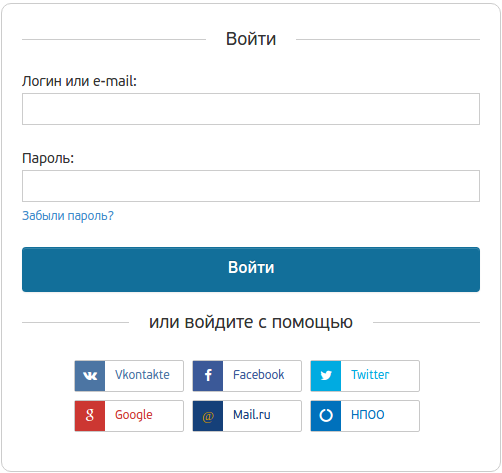
\includegraphics[height=9cm]{images/authorization/authorization_page}}
		\caption{Окно аутентификации}
		\label{img:authorization:authorization_page}
	\end{figure}
	
	В случае успеха пользователь будет перенаправлен на главную страницу Платформы, в противном случае (например, если пользователь ввёл неправильный пароль), пользователь увидит сообщение об ошибке.
	\section{Вход в АРМ вуза} \label{sec:cabinet}
Для входа в АРМ вуза необходимо нажать на значок \quotes{Мой профиль} в верхнем правом углу страницы (рис.~\ref{img:university_select:icon}),
после чего на экране появится список доступных действий.

\begin{figure}[H]
	\center{
\includegraphics[width=0.4\linewidth]{images/university_select/icon}}
	\caption{Значок \quotes{Мой профиль}}
	\label{img:university_select:icon}
\end{figure}
Если количество доступных пользователю АРМ вузов от одного до трёх, в меню будут отображены названия всех этих вузов (рис.~\ref{img:university_select:select_university_less_3}). При нажатии на любой из перечисленных в меню вузов откроется страница АРМ соответствующего вуза.

\begin{figure}[H]
	\center{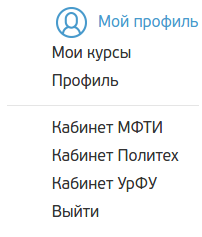
\includegraphics[width=0.4\linewidth]{images/university_select/select_university_less_3}}
	\caption{Внешний вид меню с тремя доступными вузами}
	\label{img:university_select:select_university_less_3}
\end{figure}

Если количество доступных пользователю АРМ вузов больше трёх, в меню будет отображен пункт \quotes{Кабинеты вузов} (рис.~\ref{img:university_select:select_university_more_3})

\begin{figure}[H]
	\center{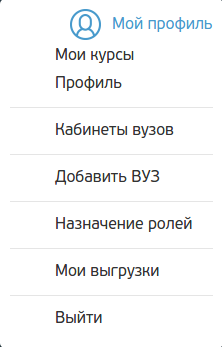
\includegraphics[width=0.4\linewidth]{images/university_select/select_university_more_3}}
	\caption{Внешний вид меню при количестве вузов более трёх}
	\label{img:university_select:select_university_more_3}
\end{figure}

При выборе данного пункта меню на экране появится окно, в котором необходимо выбрать вуз из списка (работа со списком подробно описана в пункте~\ref{widget:autocomplete}) и нажать на кнопку \vcenteredinclude[height=25px]{images/university_select/university_select_btn}, после чего пользователь будет перенаправлен в АРМ соответствующего вуза.
\begin{figure}[H]
	\center{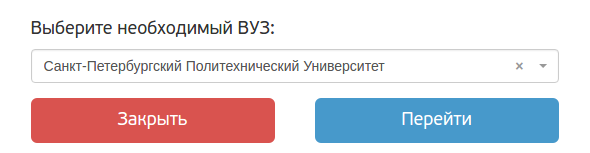
\includegraphics[width=1\linewidth]{images/university_select/select_university_dialog}}
	\caption{Окно выбора вуза}
	\label{img:university_select:select_university_dialog}
\end{figure}

Для того, что бы закрыть данный диалог, необходимо нажать на кнопку \vcenteredinclude[height=25px]{images/university_select/university_select_close_btn} или кликнуть на область вне диалога.
	\section{Типовые элементы интерфейса}
		\graphicspath{ {images/datatables/} }
\subsection{Работа с табличными представлениями} \label{sec:datatables}

Табличные данные в АРМ вуза имеют унифицированное представление и содержат следующие элементы управления:
\begin{itemize}
	\item Выбор количества записей на странице \vcenteredinclude[height=25px]{page_count}
	\item Кнопка экспорта текущей выборки в CSV-файл \vcenteredinclude[height=25px]{csv_export}
	\item Кнопка вызова диалога фильтрации \vcenteredinclude[height=25px]{filter}
	\item Строка поиска \vcenteredinclude[height=25px]{search}
	\item Элемент постраничной навигации \vcenteredinclude[height=25px]{pagination}
\end{itemize}

Пример табличных данных приведён на рис.~\ref{img:datatables:dt}

\begin{figure}[H]
	\center{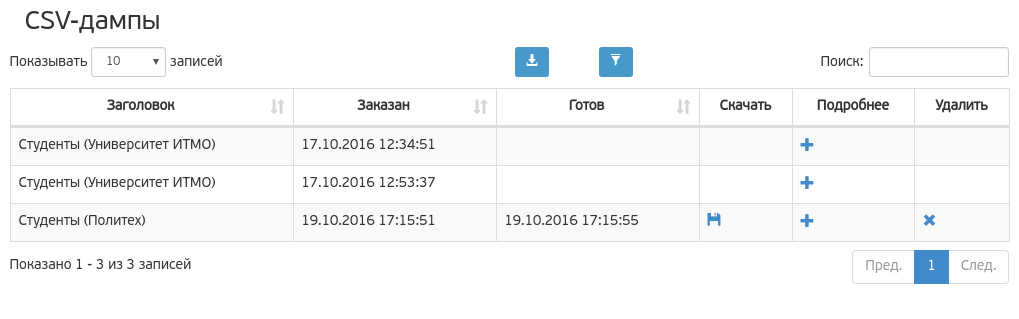
\includegraphics[width=1\linewidth]{dt}}
	\caption{Пример табличных данных}
	\label{img:datatables:dt}
\end{figure}

\subsubsection{Сортировка}

Для большинства столбцов доступна сортировка таблицы по их содержимому. Для некоторых столбцов сортировка недоступна
либо ввиду бессмысленности (в каждой ячейке находится одинаковая иконка), либо ввиду технических ограничений.
Если для столбца доступна сортировка, то в его заголовке есть значок \vcenteredinclude[height=25px]{sort_icon}.
Если таблица отсортирована по какому"=либо столбцу по убыванию, то в его заголовке есть значок \vcenteredinclude[height=25px]{sort_icon_desc},
по возрастанию "--- \vcenteredinclude[height=25px]{sort_icon_asc}.

Для сортировки по какому"=либо столбцу необходимо нажать на его заголовок. Для переключения режима сортировки <<по возрастанию>> "--- <<по убыванию>>,
необходимо повторно нажимать на заголовок того же столбца. Для сортировки по нескольким столбцам таблицы необходимо выбрать первый столбец обычным способом,
а затем нажимать на последующие при нажатой клавише \keys{\shift\ Shift}.

\subsubsection{Поиск}

В таблицах доступен поиск по содержимому всех столбцов. Для поиска текста в таблице необходимо ввести этот текст в строку поиска. Если требуется 
найти текст из нескольких слов в одном столбце, необходимо заключить этот текст в двойные или одинарные кавычки. Поиск осуществляется по мере набора текста.

\subsubsection{Фильтрация}

Во всех таблицах присутствует форма фильтрации, которую можно вызвать нажатием кнопки \vcenteredinclude[height=25px]{filter}. Для числовых полей и полей с датой в форме фильтрации предусмотрена фильтрация по диапазону. После применения фильтрации рядом с кнопкой \vcenteredinclude[height=25px]{filter} появляется кнопка \vcenteredinclude[height=25px]{filter_clear_button}.
При нажатии на неё все фильтры из формы фильтрации очищаются и таблица обновляется. 

\subsubsection{Выгрузка в CSV}

Для выгрузки табличных данных в формате CSV требуется нажать кнопку \vcenteredinclude[height=25px]{csv_export}. Данные из таблиц
сохраняются в файл в формате CSV, который может быть открыт в Microsoft Excel или LibreOffice Calc. Сортировка, фильтрация и строка
поиска учитываются при выгрузке. Если число записей менее 300, то пользователю сразу будет предложено скачать выходной файл, в противном случае файл будет выслан пользователю по почте и появится в разделе <<Мои выгрузки>>
(см.\ подраздел~\ref{sec:csv_dumps}), пользователю при этом показывается соответствующее сообщение.

		\subsection{Виджет выбора даты и времени}
\label{widget:date_time_picker}
Вызов данного виджета производится путём нажатия на кнопку \vcenteredinclude[height=25px]{images/widgets/date_time_picker_call_btn}, после чего на экране появится календарь, в котором пользователь может задать дату.
Для переключения на виджет задания времени, пользователю необходимо нажать на кнопку \vcenteredinclude[height=25px]{images/widgets/date_time_picker_time_btn}, после чего отобразится виджет выбора времени.

\subsection{Виджет загрузки файлов}
\label{widget:file_upload}
Для асинхронной загрузки файлов на сервер используется виджет загрузки файлов. Слева под меткой поля показано текущее загруженное изображение, если оно есть (см рис.~\ref{img:widgets:file_upload_ok}) или изображение по умолчанию, если ничего не загружено (см рис.~\ref{img:widget:file_upload_default_logo}). 

\begin{figure}[H]
	\center{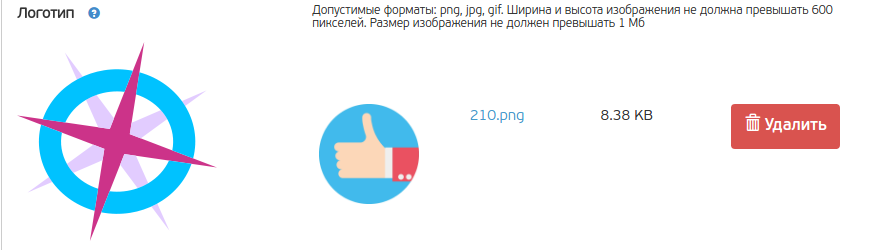
\includegraphics[width=1\linewidth]{images/widgets/file_upload_ok}}
	\caption{Успешная загрузка файла}
	\label{img:widgets:file_upload_ok}
\end{figure}

\begin{figure}[H]
	\center{
\includegraphics[width=1\linewidth]{images/widgets/file_upload_default_logo}}
	\caption{Файловое поле с изображением по умолчанию}
	\label{img:widget:file_upload_default_logo}
\end{figure}

Для того чтобы начать загрузку файла, необходимо нажать на кнопку \vcenteredinclude[height=25px]{images/widgets/file_uploat_select_file} и в окне проводника выбрать желаемый файл. Загружаемый файл должен соответствовать ограничениям на формат и размерам указанным справа от метки поля, в противном случае появится сообщение об ошибке.

\subsection{Виджет определения порядка следования записи}
\label{widget:ordering}
Виджет определения порядка следования записи представляет из себя список, элементы которого можно менять местами. Изменить порядок можно, перетащив выбранную строку на новую позицию при помощи мыши (см. рис.~\ref{img:widgect:ordered_list}).

\begin{figure}[H]
	\center{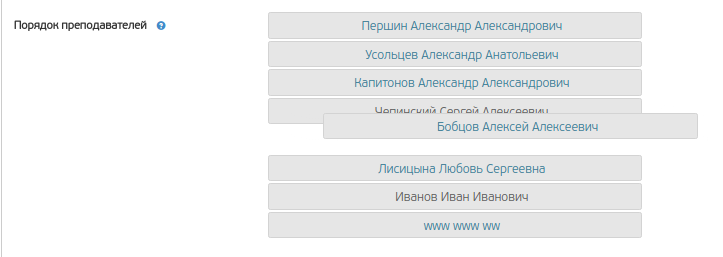
\includegraphics[width=1\linewidth]{images/widgets/ordered_list}}
	\caption{Виджет определения порядка следования записи}
	\label{img:widgect:ordered_list}
\end{figure}

В ряде случаев элементы списка можно удалять, нажав на кнопку \vcenteredinclude[height=25px]{images/widgets/delete_btn}.

\subsection{Виджет выпадающего списка с автодополнением}
\label{widget:autocomplete}
Виджет выпадающего списка предназначен для упрощения поиска. Внешний вид виджета представлен на рисунке~\ref{img:widgect:autocomplete_view} (в ряде случаев на виджете может присутствовать подсказка). При нажатии на виджет появится список значений, которые могут быть заданы в этом поле (рис.~\ref{img:widgect:autocomplete_open_view}).
\begin{figure}[H]
	\center{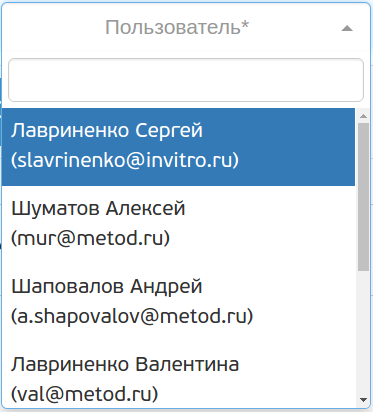
\includegraphics[width=0.5\linewidth]{images/widgets/autocomplete_open_view}}
	\caption{Внешний вид виджета при нажатии на него}
	\label{img:widgect:autocomplete_open_view}
\end{figure}

Имеется возможность фильтрации результатов путем ввода с клавиатуры части названия. Выбор необходимого результата осуществляется щелчком указателя мыши по нужному элементу в списке или по нажатию клавиши \keys{\enter} (в последнем случае будет выбран выделенный элемент списка). Для того что бы отменить выбор, необходимо нажать клавишу \keys{\esc} или кликнуть курсором мыши вне виджета. Очистка поля производится нажатием на \quotes{X}.

	\graphicspath{{images/university/}}
\section{Об университете}
	Раздел позволяет просматривать и редактировать информацию, связанную с университетом: основную информацию, контакты, а также медиа"=файлы, отвечающие за отображение страниц, связанных с этим вузом на сайте.
	
	\subsection{Роли и операции}
	
	Раздел доступен пользователям, имеющим следующие роли:	

	\begin{itemize}
		\item Администратор Платформы:
		\begin{itemize}
			\item просмотр информации об университете;
			\item редактирование информации об университете;
			\item создание нового университета.
		\end{itemize}
		\item Администратор вуза"=поставщика:
		\begin{itemize}
			\item просмотр информации об университете;
			\item редактирование информации об университете.
		\end{itemize}
		\item Администратор контента вуза"=поставщика:
		\begin{itemize}
			\item просмотр информации об университете;
			\item редактирование информации об университете.
		\end{itemize}
	\end{itemize} 
	
	\subsection{Просмотр информации об университете}\label{university:detail_section}
	При выборе в главном меню пункта \quotes{Об университете} загружается подраздел \quotes{Просмотр информации}, в котором доступны для просмотра все имеющиеся на текущий момент данные об университете.

	Внешний вид подраздела приведён на рисунке~\ref{university:detailview}
	
	\begin{figure}[H]
	\center{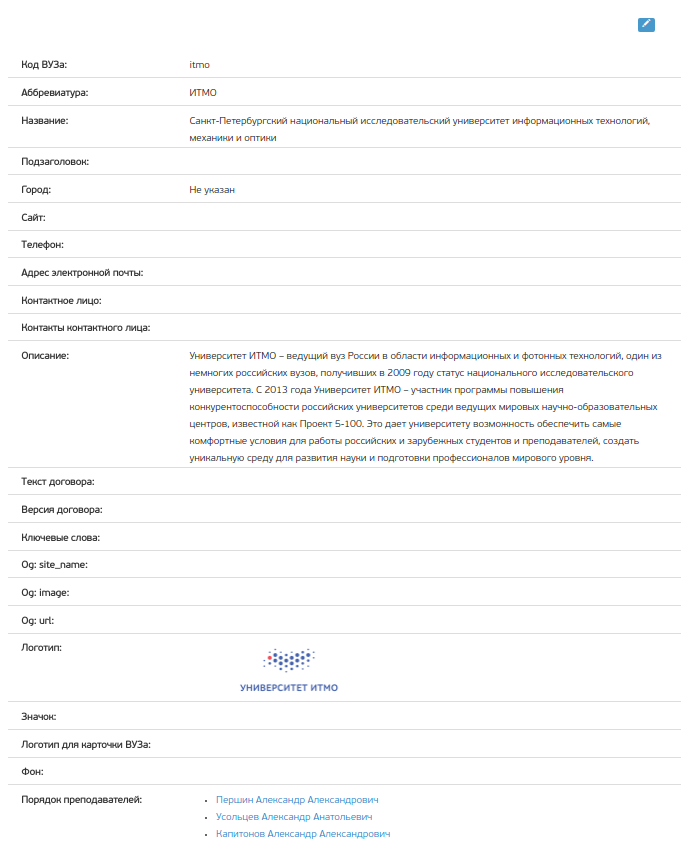
\includegraphics[width=1\linewidth]{detailview.png}}
	\caption{Внешний вид подраздела \quotes{Просмотр информации}}
	\label{university:detailview}
	\end{figure}
	
	Для просмотра доступны следующие поля:
	\begin{itemize}
		\item код вуза "--- уникальный код университета на Платформе, заполняется при создании вуза, неизменяем;
		\item аббревиатура;
		\item полное название университета;
		\item подзаголовок "--- краткое название университета;
		\item город;
		\item сайт;
		\item телефон;
		\item e"=mail;
		\item контактное лицо по умолчанию для связи по договорам, заключаемым данным университетом;
		\item контакты контактного лица (e"=mail, номер телефона, др.);
		\item описание университета;
		\item текст договора, согласие с которым должен подтвердить студент для того, чтобы получить доступ к курсам данного университета;
		\item версия договора, с которым соглашается студент при записи на курс;
		\item метаданные: ключевые слова, og:site\_name, og:image, og:url;
		\item логотип университета;
		\item значок;
		\item логотип для карточки вуза;
		\item фон;
		\item порядок преподавателей "--- список преподавателей в том порядке, в котором они будут показываться на странице университета на сайте, элемент списка "--- ссылка, ведущая на страницу просмотра подробной информации о конкретном преподавателе.
	\end{itemize}

	\subsection{Редактирование информации об университете}\label{university:edit}
	Для перехода к подразделу редактирования необходимо нажать на иконку \quotes{редактирование} \vcenteredinclude[width=0.1\linewidth]{edit_icon.png} в верхнем правом углу страницы подраздела \quotes{Просмотр информации} (рис.~\ref{university:detailview}).

	
	В этом случае осуществляется переход к форме редактирования университета, в которой можно изменять поля, описанные в разделе~\ref{university:detail_section}. 
	
	\subsubsection{Поля и ошибки}
	В форме представлено несколько типов полей:
	\begin{itemize}
		\item \textbf{Обязательные поля} отмечены символом \quotes{*}, если такое поле оставить не заполненным "--- появляется сообщение о необходимости его заполнения и блокируется кнопка сохранения изменений (см. рис.~\ref{university:edit_required}).
		
		\begin{figure}[H]
		\center{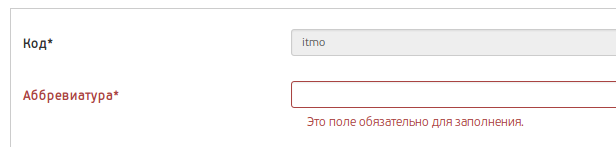
\includegraphics[width=1\linewidth]{edit_required.png}}
		\caption{Обработка заполнения обязательных полей}
		\label{university:edit_required}
		\end{figure}	
	
		\item \textbf{Сайт и адрес электронной почты университета}. Ввод информации в эти поля необходимо осуществлять в корректном формате, например, \texttt{http://npoed.ru} для сайта и \texttt{npoed@mail.ru} для почты соответственно, в противном случае появится сообщение об ошибке и будет заблокирована кнопка сохранения изменений (см. рис.~\ref{university:edit_url_email})
		
		\begin{figure}[H]
		\center{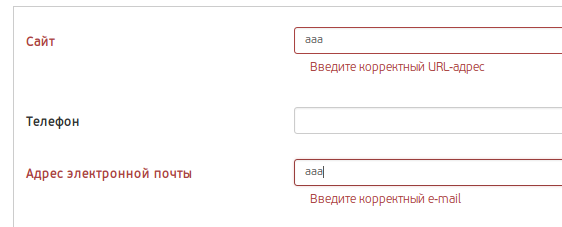
\includegraphics[width=1\linewidth]{edit_url_email.png}}
		\caption{Обработка заполнения полей \quotes{Сайт} и \quotes{Адрес электронной почты}}
		\label{university:edit_url_email}
		\end{figure}	
		
		\item \textbf{Поле \quotes{порядок преподавателей}} представляет собой список ФИО преподавателей университета в том порядке, в котором они будут показаны на сайте. Описание работы с виджетом изменения порядка см. в подразделе~\ref{widget:ordering}

		Для каждого преподавателя отдельно можно настроить его видимость на сайте в подразделе редактирование преподавателя путем переключения значения поля \quotes{Опубликован}, неопубликованные преподаватели скрыты на сайте для пользователей. В форме редактирования университета в списке преподавателей показываются как скрытые, так и опубликованные преподаватели. В зависимости от статуса их ФИО имеют различный цвет. Подробное описание можно получить, нажав на иконку \quotes{помощь} рядом с меткой поля (см. рис.~\ref{university:edit_instructors_legend}).
		
		\begin{figure}[H]
		\center{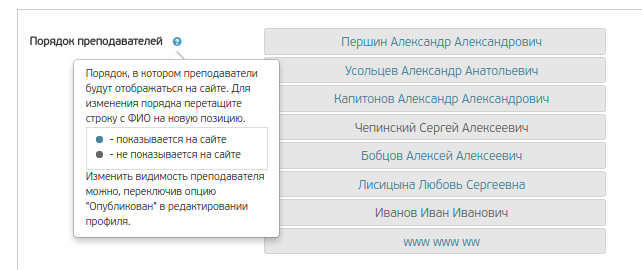
\includegraphics[width=1\linewidth]{edit_instructors_legend.png}}
		\caption{Справка о статусе преподавателей}
		\label{university:edit_instructors_legend}
		\end{figure}	
		
		\item \textbf{Файлы}. Форма редактирования позволяет загружать изображения для формирования внешнего вида страницы университета на сайте. Слева под меткой поля показано текущее загруженное изображение, если оно есть (см рис.~\ref{university:edit_logo}) или изображение по умолчанию, если ничего не загружено (см рис.~\ref{university:edit_icon_image}). Подробная информация по работе с файловыми полями приведена в разделе~\ref{widget:file_upload}.

		\begin{figure}[H]
		\center{
\includegraphics[width=1\linewidth]{edit_logo.png}}
		\caption{Файловое поле с загруженным изображением}
		\label{university:edit_logo}
		\end{figure}	
		
		\begin{figure}[H]
		\center{
\includegraphics[width=1\linewidth]{edit_icon_image.png}}
		\caption{Файловое поле с изображением по умолчанию}
		\label{university:edit_icon_image}
		\end{figure}
\end{itemize}

	\subsubsection{Элементы управления}\label{university:edit_save_cancel}
Управление внесенными изменениями осуществляется с помощью кнопок, расположенных внизу страницы (см. рис.~\ref{university:edit_buttons}).
		\begin{figure}[H]
		\center{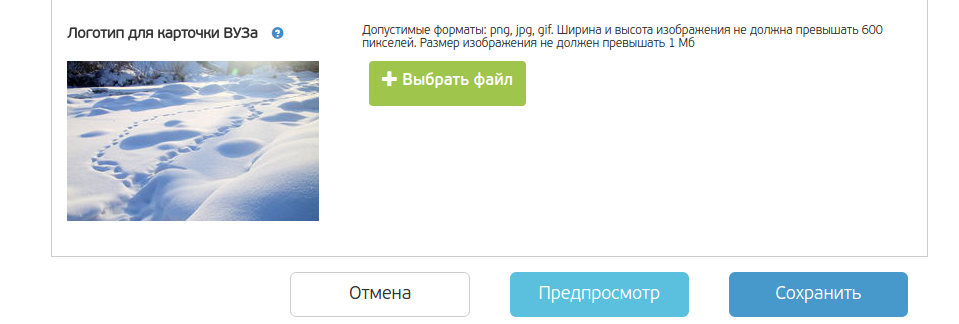
\includegraphics[width=1\linewidth]{edit_buttons.png}}
		\caption{Элементы управления подраздела редактирования}
		\label{university:edit_buttons}
		\end{figure}	
		
При нажатии \quotes{сохранить} осуществляется попытка сохранения формы: если форма заполнена корректно, то внесенные изменения сохраняются, пользователь перенаправляется в раздел \quotes{просмотр информации об университете}, в противном случае, если имеются ошибки, отображаются сообщения об ошибках, осуществляется прокрутка к месту первой ошибки. 


При нажатии кнопки \quotes{отмена} все изменения теряются, пользователь перенаправляется на предыдущую страницу.


Действия, вызываемые по нажатию кнопки \quotes{предпросмотр}, описаны в разделе~\ref{university:edit_preview_ch}
	
	\subsubsection{Предпросмотр}\label{university:edit_preview_ch}
	Для подраздела \quotes{Редактирование университета} доступна опция предпросмотра, с помощью которой можно оценить внешний вид страницы университета на сайте для пользователей с учётом внесенных изменений. Предпросмотр можно осуществить даже в том случае, если форма заполнена некорректно или не полностью. Страница загружается во всплывающем окне при нажатии кнопки \quotes{Предпросмотр} внизу страницы с формой редактирования (см. рис.~\ref{university:edit_preview}). При этом все внешние ссылки на отображаемой странице заблокированы.
	
		\begin{figure}[H]
		\center{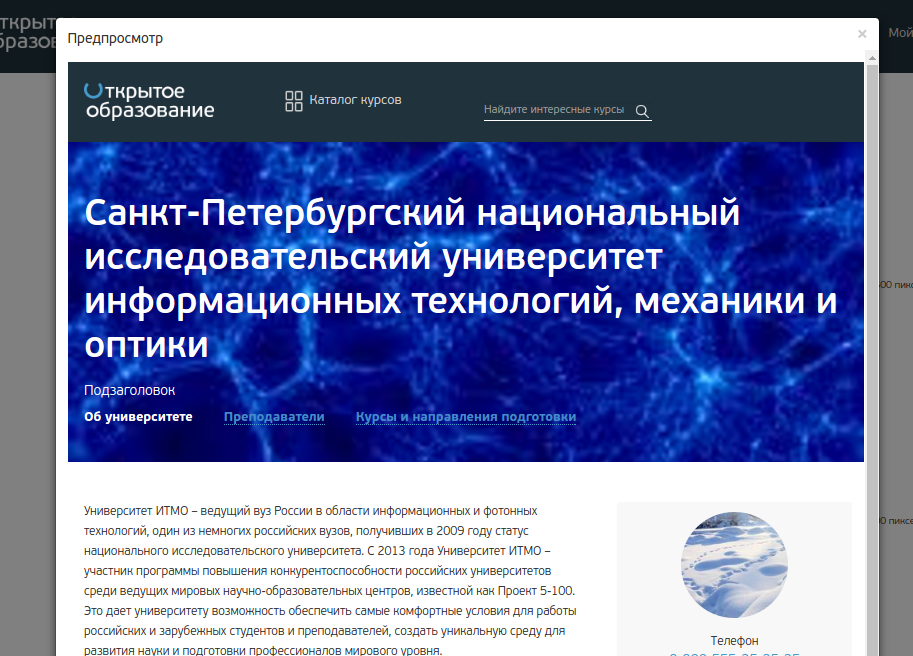
\includegraphics[width=1\linewidth]{edit_preview.png}}
		\caption{Окно предпросмотра}
		\label{university:edit_preview}
		\end{figure}	

Закрыть окно предпросмотра можно нажатием за пределы окна, либо по нажатию кнопки \quotes{закрыть} внизу окна, либо по нажатию крестика [х] в верхнем правом углу окна. Также из окна можно осуществить попытку сохранения внесенных изменений путем нажатия на кнопку \quotes{сохранить} в нижней части окна (см. рис.~\ref{university:edit_preview_button}). При этом поведение будет такое же, как при попытке сохранения из формы редактирования (см.~\ref{university:edit_save_cancel}).

		\begin{figure}[H]
		\center{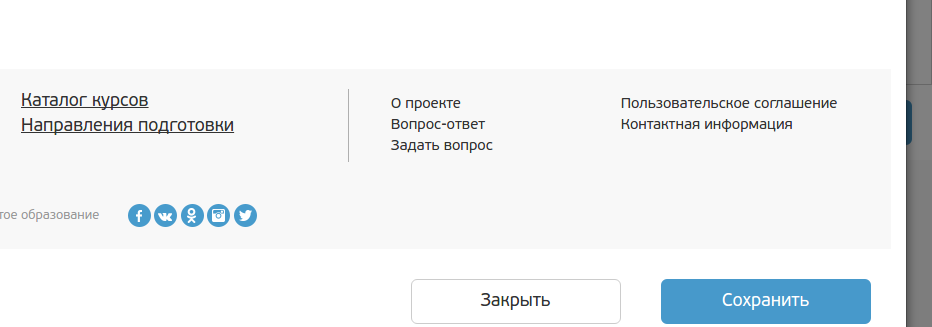
\includegraphics[width=1\linewidth]{edit_preview_button.png}}
		\caption{Элементы управления окна предпросмотра}
		\label{university:edit_preview_button}
		\end{figure}	
		
\subsection{Создание университета}
Возможность создания кабинета университета доступна администратору Платформы. 

Для перехода в подраздел необходимо выбрать в меню \quotes{Мой профиль}, расположенном в верхнем правом углу страницы, пункт \quotes{добавить вуз} (см. рис.~\ref{university:create_menu}).

		\begin{figure}[H]
		\center{
\includegraphics[width=1\linewidth]{create_menu.png}}
		\caption{Выбор пункта \quotes{Добавить вуз} в меню пользователя}
		\label{university:create_menu}
		\end{figure}	
		
В этом случае осуществляется переход к форме создания университета, в которой возможно задать значения полей, описанных в разделе~\ref{university:detail_section}. Содержание, возможные действия и реакции в этом разделе аналогичны описанным в разделе \quotes{Редактирование информации об университете}~\ref{university:edit} за исключением двух моментов:
\begin{itemize}
	\item В форме создания задается уникальный код университета на Платформе (поле \quotes{Код}), который в последствие не может быть изменен. При нажатии на поле ввода появляется подсказка о требуемом формате кода (см. рис.~\ref{university:create_slug_help}). При несоответствии введенного кода этому формату появится сообщение об ошибке. Также необходимым условием валидности кода является его уникальность, при наборе уже существующего на Платформе значения появится сообщение об ошибке (см. рис.~\ref{university:create_slug_exist}). Поле \quotes{Код} является обязательным.
	
		\begin{figure}[H]
		\center{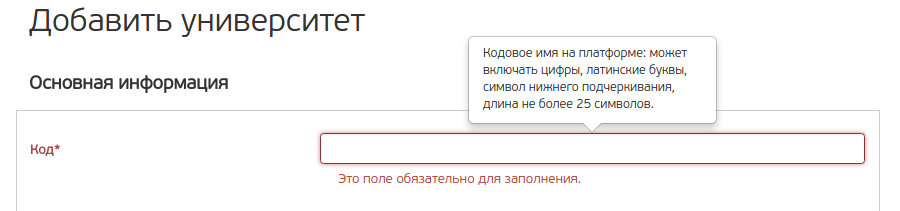
\includegraphics[width=1\linewidth]{create_slug_help.png}}
		\caption{Сообщение"=подсказка о формате кода университета}
		\label{university:create_slug_help}
		\end{figure}
		
		\begin{figure}[H]
		\center{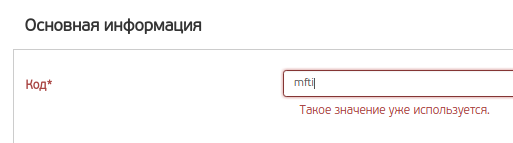
\includegraphics[width=1\linewidth]{create_slug_exist.png}}
		\caption{Сообщение об ошибке: введенный код уже занят}
		\label{university:create_slug_exist}
		\end{figure}	
		
	\item Вторым отличием от формы редактирования является отсутствие списка преподавателей. Они добавляются после создания университета через раздел \quotes{Преподаватели}, и после добавления отображаются в разделах \quotes{Просмотр информации об университете}, \quotes{Редактирование университета}, \quotes{Преподаватели}.
\end{itemize}
	
	

		

	
	
	
	
	
	
	\graphicspath{{images/instructor/}}

\section{Преподаватели}
Для перехода в раздел необходимо нажать пункт \quotes{Преподаватели} на главной панели (выделен на рисунке~\ref{instructor:instructor_section} ), пункт доступен в том случае, если вуз не является только потребителем, в противном случае он скрыт.

\begin{figure}[H]
	\center{
\includegraphics[width=1\linewidth]{instructor_section.png}}
	\caption{Выбор раздела \quotes{Преподаватели}}
	\label{instructor:instructor_section}
\end{figure}

Раздел включает в себя сведения о преподавателях конкретного вуза. С помощью средств раздела можно просматривать, редактировать информацию о существующих преподавателях и добавлять новых преподавателей к университету. При выборе раздела в главном меню открывается подраздел \quotes{Список преподавателей}.

\subsection{Роли и операции}
Раздел доступен из кабинетов вузов, которые не являются только потребителями, пользователям, имеющим следующие роли:
\begin{itemize}
	\item Администратор вуза;
	\item Администратор контента вуза;
\end{itemize}

Для пользователя с любой из перечисленных выше ролей доступны следующие действия:
\begin{itemize}
	\item просмотр списка преподавателей;
	\item просмотр профиля преподавателя;
	\item редактирование профиля преподавателя;
	\item добавление преподавателя;
	\item удаление преподавателя.
\end{itemize}

\subsection{Список преподавателей}
При выборе на главной панели пункта \quotes{Преподаватели} загружается подраздел \quotes{Список преподавателей}, в котором доступны для просмотра в кратком виде данные обо всех преподавателях вуза и элементы для перехода к другим подразделам.

Внешний вид подраздела приведён на рисунке~\ref{instructor:list}. 

	\begin{figure}[H]
	\center{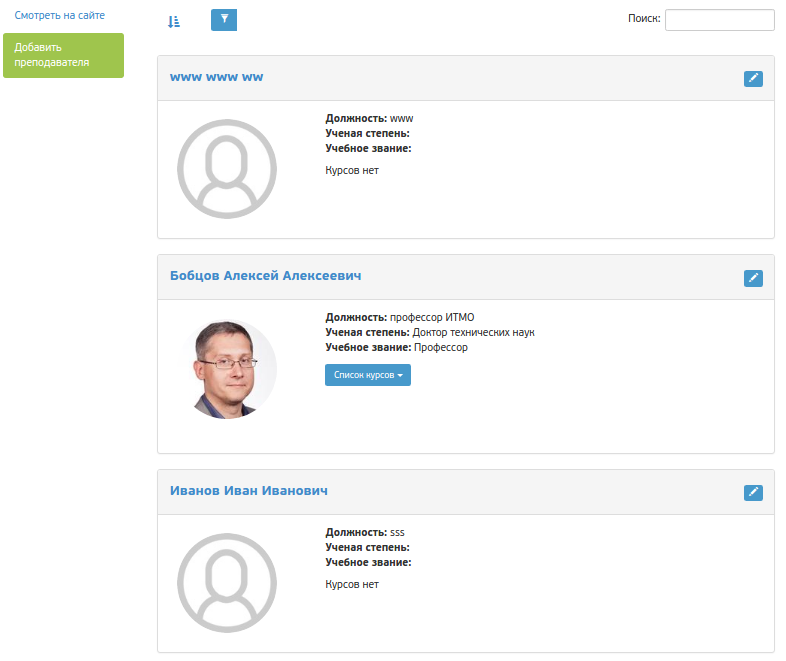
\includegraphics[width=1\linewidth]{list.png}}
	\caption{Внешний вид подраздела \quotes{Список преподавателей}}
	\label{instructor:list}
	\end{figure}
	
В центральной части страницы выводится непосредственно список преподавателей, каждый элемент которого "--- блок с краткой информацией о конкретном преподавателе. В левом углу верхней панели блока ФИО является ссылкой, ведущей в подраздел \quotes{Просмотр профиля преподавателя}, в правом углу "--- иконка редактирования, нажатие которой переводит в подраздел \quotes{Редактирование профиля преподавателя}. В основной части блока показаны:
\begin{itemize}
	\item фотография профиля, если она загружена или изображение по умолчанию, если отсутствует;
	\item должность преподавателя в вузе;
	\item ученая степень;
	\item учебное звание;
	\item список курсов. (показать/скрыть список курсов можно нажатием на кнопку \quotes{Список курсов} в блоке соответствующего преподавателя).
\end{itemize}

Вид блока с развернутым списком курсов приведён на рисунке~\ref{instructor:list_courses}.
	
	\begin{figure}[H]
	\center{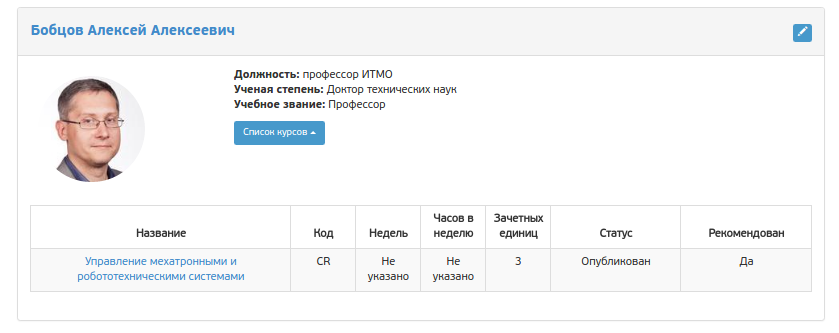
\includegraphics[width=1\linewidth]{list_courses.png}}
	\caption{Вид элемента списка преподавателей}
	\label{instructor:list_courses}
	\end{figure}

\subsubsection{Элементы управления}
На странице списка преподавателей присутствуют следующие элементы управления:
\begin{itemize}
	\item Кнопки \quotes{Смотреть на сайте} и \quotes{Добавить преподавателя}. Расположены на панели слева от списка преподавателей (см. рис.~\ref{instructor:list}). По нажатию кнопки \quotes{Смотреть на сайте} происходит перенаправление на страницу университета на сайте, которая видна для пользователей. \\
	По нажатию кнопки \quotes{Добавить преподавателя} происходит перенаправление в соответствующий раздел.
	\item \vcenteredinclude[width=0.1\linewidth]{list_order.png} "--- иконка изменения порядка отображения преподавателей. 


По умолчанию список отсортирован в алфавитном порядке по ФИО в направлении А--Я, нажатие на иконку изменяет порядок на противоположный.
	\item \vcenteredinclude[width=0.1\linewidth]{list_filter_icon.png} "--- иконка вызова формы фильтрации.

 
По умолчанию в списке показаны все преподаватели вуза, однако, можно осуществить фильтрацию и вывести только тех, которые удовлетворяют параметрам, указным в форме фильтрации. По нажатию на иконку вызова формы фильтрации всплывает окно с формой фильтрации, в которой можно задать интересующие параметры (см. рис.~\ref{instructor:list_filter_form}). 

	\begin{figure}[H]
	\center{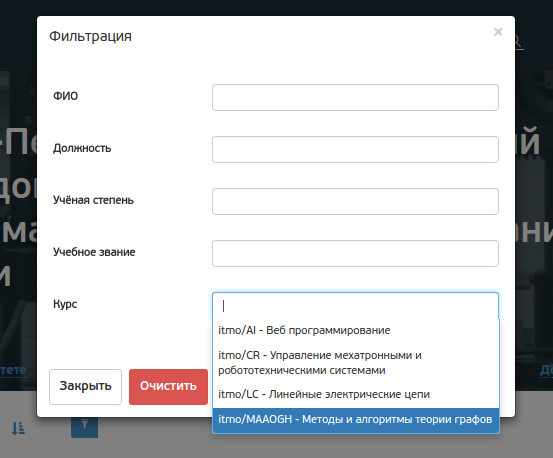
\includegraphics[width=1\linewidth]{list_filter_form.png}}
	\caption{Форма фильтрации}
	\label{instructor:list_filter_form}
	\end{figure}

Форма содержит следующие поля:
\begin{itemize}
	\item ФИО преподавателя (для поиска можно вводить любые части и комбинации фамилии, имени, отчества);
	\item должность;
	\item учёная степень;
	\item учебное звание;
	\item курс (принципы работы с полями такого типа описаны в подразделе ~\ref{widget:autocomplete_with_multiselect});
\end{itemize}	

Для того, чтобы применить фильтр необходимо нажать кнопку формы \quotes{Фильтровать}, после этого в списке останутся только преподаватели, удовлетворяющие введенным параметрам, а на верхней панели подраздела появится красная иконка \quotes{Отменить фильтр} \vcenteredinclude[width=0.2\linewidth]{list_filter_cancel.png}


Нажатие на иконку  \vcenteredinclude[width=0.06\linewidth]{del_filter_icon.png} отменяет применённый фильтр, в списке снова отображаются все преподаватели.
Пример результата фильтрации приведён на рисунке~\ref{instructor:list_filter_result}.

	\begin{figure}[H]
	\center{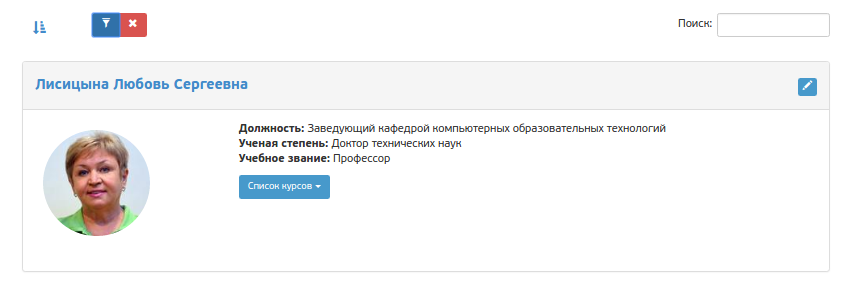
\includegraphics[width=1\linewidth]{list_filter_result.png}}
	\caption{Результат применения фильтра}
	\label{instructor:list_filter_result}
	\end{figure}
	
	\item \vcenteredinclude[width=0.3\linewidth]{quick_search.png} "--- поле быстрого поиска расположено в правом углу верхней панели раздела, справа от метки \quotes{Поиск}. Поиск осуществляется по ФИО преподавателя, при заполнении поля выводятся только те преподаватели, чьи ФИО содержат введенную в поле строку (см. рис. ~\ref{instructor:list_search}).
	
	\begin{figure}[H]
	\center{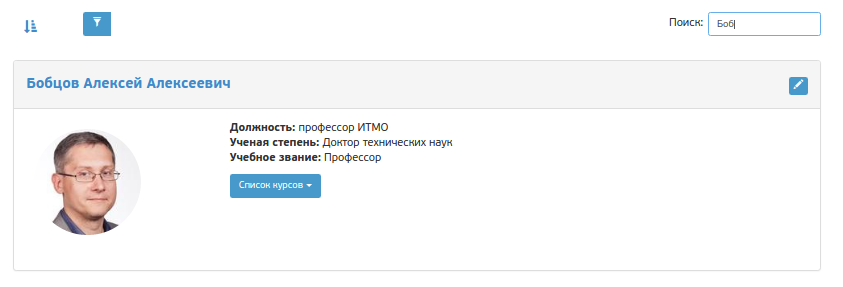
\includegraphics[width=1\linewidth]{list_search.png}}
	\caption{Применение быстрого поиска}
	\label{instructor:list_search}
	\end{figure}
	
	\item \vcenteredinclude[width=0.3\linewidth]{list_pagination.png} "--- элемент постраничной навигации          
 расположен внизу страницы раздела. На одной странице выводятся пять элементов списка, для перехода на следующую/предыдущую страницу используются стрелки вправо/влево.
	
\end{itemize}


\subsection{Просмотр профиля преподавателя}\label{instructor:detail_section}
По нажатию на ФИО интересующего преподавателя в списке преподавателей открывается относящийся к нему подраздел \quotes{Просмотр профиля преподавателя}, в котором доступны для просмотра все имеющиеся на текущий момент данные о преподавателе:
\begin{itemize}
	\item фото;
	\item ФИО;
	\item должность;
	\item ученая степень;
	\item учебное звание;
	\item образование;
	\item описание;
	\item профессиональный опыт;
	\item награды и достижения;
	\item внешние ресурсы;
	\item номер в списке преподавателей (на сайте преподаватели выводятся в порядке, соответствующем их номерам, по возрастанию номеров);
	\item опубликован "--- cтатус видимости преподавателя на сайте. (если значение статуса \quotes{Да} "--- преподаватель виден на сайте, иначе "--- скрыт);
	\item курсы (если на портале есть курсы, относящиеся к этому преподавателю, то на странице отображается таблица, содержащая информацию об этих курсах).
\end{itemize}
Также в нижней части страницы имеется кнопка \quotes{Удалить преподавателя}, которая позволяет произвести попытку удаления преподавателя. \\
Внешний вид подраздела приведён на рисунке~\ref{instructor:detail}.

	\begin{figure}[H]
	\center{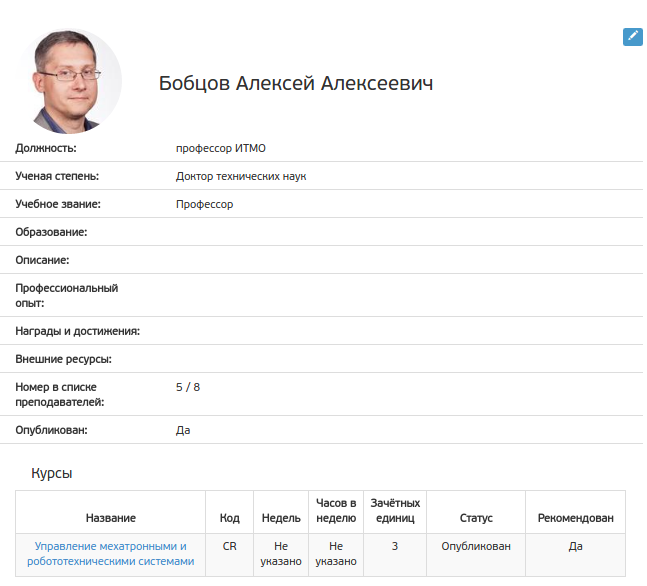
\includegraphics[width=1\linewidth]{detail.png}}
	\caption{Внешний вид подраздела \quotes{Просмотр профиля преподавателя}}
	\label{instructor:detail}
	\end{figure}
	
\subsection{Удаление преподавателя}\label{instructor:delete_section}
Для того, чтобы произвести попытку удаления преподавателя, необходимо нажать кнопку \quotes{Удалить преподавателя} в нижней части страницы раздела \quotes{Просмотр профиля преподавателя} (см. рис.~\ref{instructor:detail}). По нажатию этой кнопки будет показано модальное окно с подтверждением действия и информацией о связанных с удаляемым преподавателем объектах.\\
Если преподаватель назначен в команду какого-либо курса, то в модальном окне будет выведена информация о том, что после удаления преподаватель также будет удален из этого курса и всех его сессий см. рис.~\ref{instructor:del_with_courses}.

\begin{figure}[H]
	\center{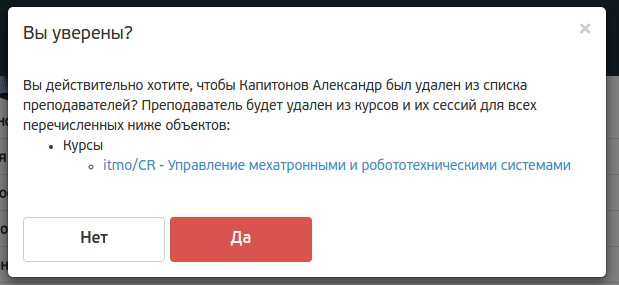
\includegraphics[width=1\linewidth]{del_with_courses.png}}
	\caption{Окно подтверждения удаления преподавателя, упомянутого в команде курса}
	\label{instructor:del_with_courses}
\end{figure}

Если преподаватель не указан в команде какого-либо курса, модальное окно будет содержать только вопрос о подтверждении удаления см. рис.~\ref{instructor:del_no_courses}.

\begin{figure}[H]
	\center{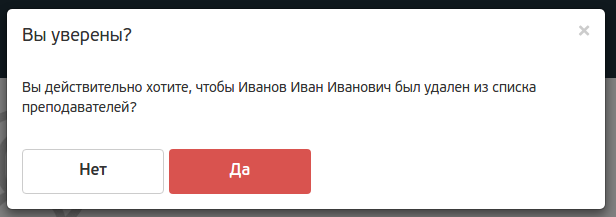
\includegraphics[width=1\linewidth]{del_no_courses.png}}
	\caption{Окно подтверждения удаления преподавателя,не упомянутого в команде курса}
	\label{instructor:del_no_courses}
\end{figure}

Для того, чтобы прервать операцию удаления достаточно нажать кнопку \quotes{Нет} или "X" в правом верхнем углу модального окна, или нажать за пределы окна. В этом случае модальное окно закроется, пользователь останется на странице \quotes{Просмотр профиля преподавателя}.\\

Чтобы подтвердить удаление необходимо нажать кнопку \quotes{Да} в модальном окне. После этого будет произведено удаление преподавателя из университета, вся информация о нем будет стерта, в том числе упоминания в команде курсов и сессий. Пользователь будет перенаправлен в раздел \quotes{Список преподавателей}.
	
\subsection{Редактирование профиля преподавателя}\label{instructor:edit_section}
Перейти в этот подраздел можно, нажав иконку редактирования \vcenteredinclude[width=0.1\linewidth]{edit_icon.png} в блоке преподавателя в списке или в верхнем правом углу подраздела \quotes{Просмотр профиля преподавателя}.


В этом случае осуществляется переход к форме редактирования профиля преподавателя, в которой можно изменять поля, описанные в подразделе~\ref{instructor:detail_section} за исключением курсов, редактирование которых осуществляется в разделе \quotes{Курсы}. 

\subsubsection{Поля и ошибки}
	В форме представлено несколько типов полей:
	\begin{itemize}
		\item \textbf{Обязательные поля} отмечены символом \quotes{*}, если такое поле оставить не заполненным "--- появляется сообщение о необходимости его заполнения и блокируется кнопка сохранения изменений (см. рис.~\ref{instructor:edit_required}).
		
		\begin{figure}[H]
		\center{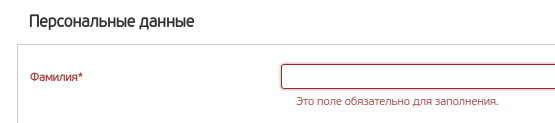
\includegraphics[width=1\linewidth]{edit_required.png}}
		\caption{Обработка заполнения обязательных полей}
		\label{instructor:edit_required}
		\end{figure}	
		
		\item \textbf{Поле \quotes{Порядок преподавателей}} представляет собой список ФИО преподавателей, относящихся к тому же университету, что и тот, чей профиль редактируется. ФИО отображаются в том порядке, в котором они будут показаны на сайте, изменить порядок можно, перетащив стрелкой мыши выбранную строку на новую позицию. Строка с редактируемым преподавателем выделена границей и более темным фоном (см. рис.~\ref{instructor:edit_instructors}). Описание работы с виджетом изменения порядка см. в подразделе~\ref{widget:ordering}.
		
		\begin{figure}[H]
		\center{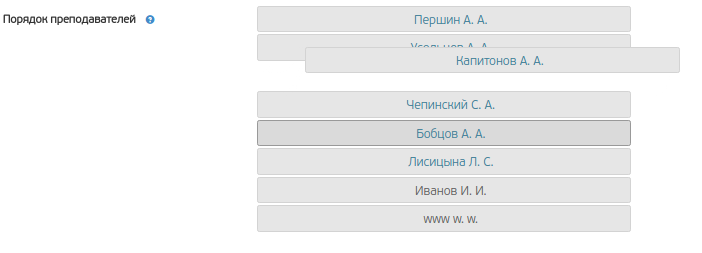
\includegraphics[width=0.8\linewidth]{edit_instructors.png}}
		\caption{Изменение порядка преподавателей}
		\label{instructor:edit_instructors}
		\end{figure}	
		
Видимость преподавателя на сайте настраивается путем переключения значения поля \quotes{Опубликован}. Неопубликованные преподаватели скрыты на сайте для пользователей. В форме в списке преподавателей показываются как скрытые, так и опубликованные преподаватели. В зависимости от статуса их ФИО имеют различный цвет, подробное описание можно получить, нажав на иконку \vcenteredinclude[width=0.06\linewidth]{help_icon.png} рядом с меткой поля (см. рис.~\ref{instructor:edit_instructors_legend}).
		
		\begin{figure}[H]
		\center{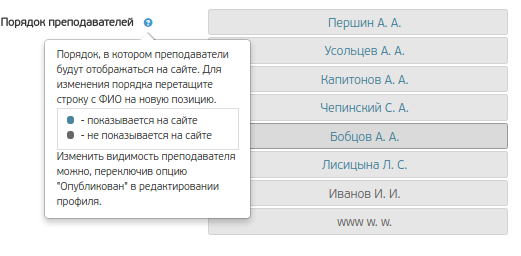
\includegraphics[width=1\linewidth]{edit_instructors_legend.png}}
		\caption{Справка о статусе преподавателей}
		\label{instructor:edit_instructors_legend}
		\end{figure}	
		
		\item \textbf{Файлы}. Форма редактирования позволяет загрузить фото профиля для отображения на страницах университета  и курсов преподавателя. Слева под меткой поля показано текущее загруженное изображение, если оно есть (см рис.~\ref{instructor:edit_logo}) или изображение по умолчанию, если ничего не загружено (см рис.~\ref{instructor:edit_icon_image}). Подробная информация о работе с файловыми полями приведена в разделе~\ref{widget:file_upload}.
		
		\begin{figure}[H]
		\center{
\includegraphics[width=1\linewidth]{edit_logo.png}}
		\caption{Файловое поле с загруженным изображением}
		\label{instructor:edit_logo}
		\end{figure}	
		
		\begin{figure}[H]
		\center{
\includegraphics[width=1\linewidth]{edit_icon_image.png}}
		\caption{Файловое поле с изображением по умолчанию}
		\label{instructor:edit_icon_image}
		\end{figure}
\end{itemize}

	\subsubsection{Элементы управления}

Управление внесенными изменениями осуществляется с помощью кнопок, расположенных внизу страницы (см. рис.~\ref{instructor:edit_buttons}).
		\begin{figure}[H]
		\center{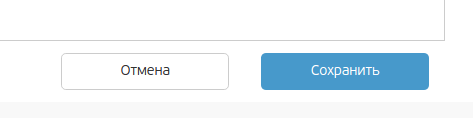
\includegraphics[width=1\linewidth]{edit_buttons.png}}
		\caption{Элементы управления подраздела \quotes{Редактирование профиля преподавателя}}
		\label{instructor:edit_buttons}
		\end{figure}	
		
При нажатии \quotes{Сохранить} осуществляется попытка сохранения формы: если форма заполнена корректно, то внесенные изменения сохраняются, пользователь перенаправляется в раздел \quotes{Просмотр профиля преподавателя}, в противном случае "--- отображаются сообщения об ошибках, осуществляется прокрутка к месту первой ошибки. 


При нажатии кнопки \quotes{Отмена} все изменения теряются, пользователь перенаправляется на предыдущую страницу.

Действия, вызываемые по нажатию кнопки \quotes{Предпросмотр}, описаны в разделе~\ref{instructor:edit_preview_ch}

\subsubsection{Предпросмотр}\label{instructor:edit_preview_ch}
Для подраздела \quotes{Редактирование профиля преподавателя} доступна опция предпросмотра, с помощью которой можно оценить внешний вид страницы преподавателя на сайте для пользователей с учётом внесённых изменений. Предпросмотр можно осуществить даже в том случае, если форма заполнена некорректно или не полностью. Страница загружается во всплывающем окне при нажатии кнопки \quotes{Предпросмотр} внизу страницы с формой редактирования (см. рис.~\ref{instructor:edit_preview}). При этом все внешние ссылки на отображаемой странице заблокированы.

\begin{figure}[H]
	\center{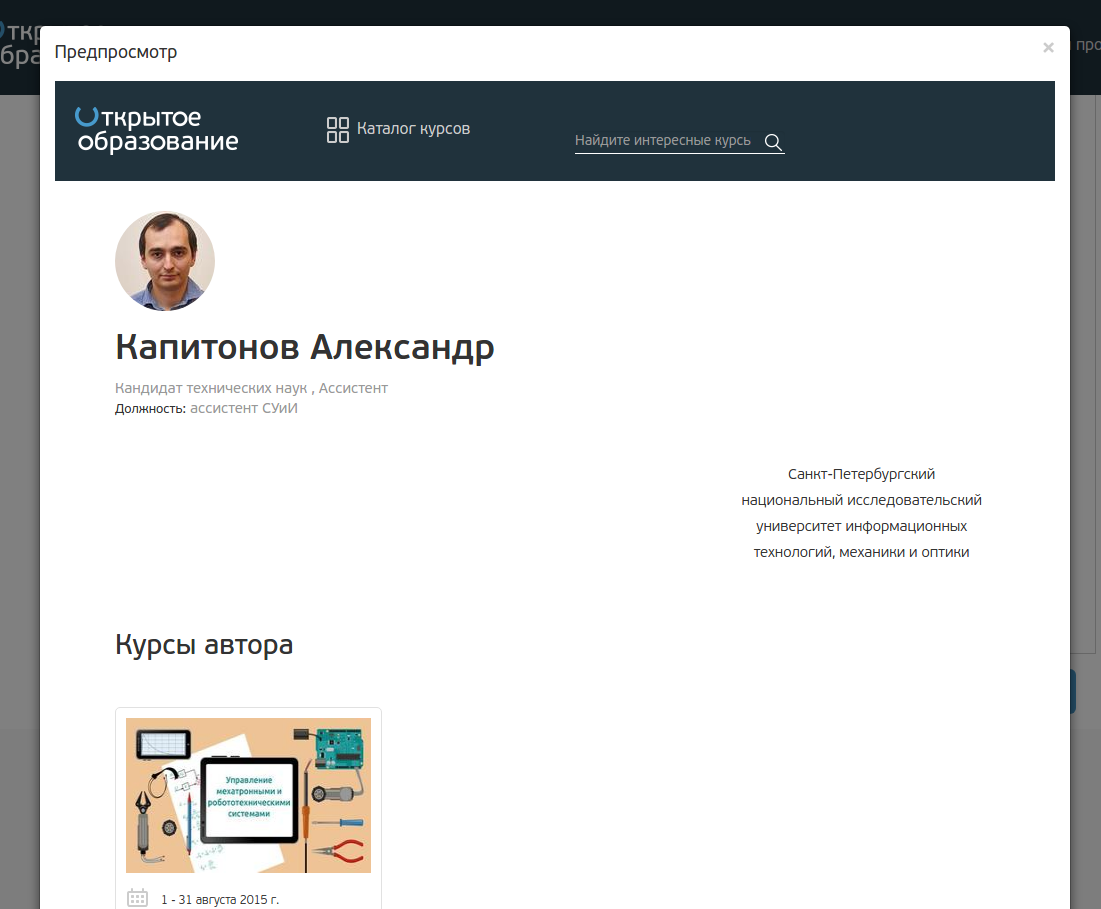
\includegraphics[width=1\linewidth]{edit_preview.png}}
	\caption{Окно предпросмотра}
	\label{instructor:edit_preview}
\end{figure}	

Закрыть окно предпросмотра можно нажатием за пределы окна, либо по нажатию кнопки \quotes{Закрыть} внизу окна (см. рис.~\ref{instructor:preview_close_button}), либо по нажатию крестика в верхнем правом углу окна. 

\begin{figure}[H]
	\center{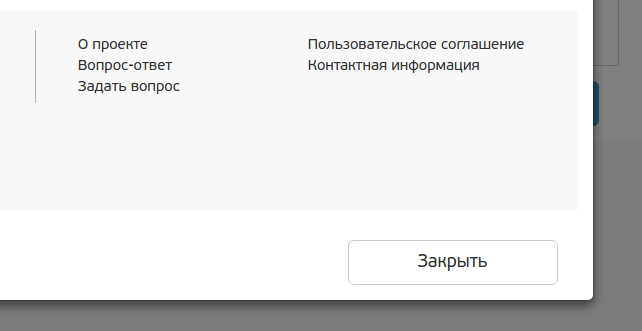
\includegraphics[width=1\linewidth]{preview_close_button.png}}
	\caption{Кнопка закрытия окна предпросмотра}
	\label{instructor:preview_close_button}
\end{figure}


\subsection{Добавление преподавателя}
Перейти к созданию преподавателя можно, нажав на кнопку \quotes{Добавить преподавателя}, которая размещена на левой панели во всех подразделах раздела \quotes{Преподаватели}. В этом случае осуществляется переход к форме создания нового преподавателя, в которой возможно задать значения полей, описанных в разделе~\ref{instructor:detail_section}. Содержание, возможные действия и реакции в этом разделе аналогичны описанным в разделе \quotes{Редактирование профиля преподавателя}~\ref{instructor:edit_section} за исключением вида поля \quotes{Порядок преподавателей}.



\textbf{Поле \quotes{Порядок преподавателей}} представляет собой список ФИО преподавателей, относящихся к университету, в кабинете которого находится пользователь. Строка, описывающая нового преподавателя, вместо ФИО содержит текст \quotes{Добавить на эту позицию}, кроме того, она выделена среди остальных более темным цветом фона и темной границей.


Строки отображаются в порядке, в котором преподаватели будут показаны на сайте, новый преподаватель по умолчанию помещается на последнюю позицию, изменить порядок можно, перетащив  при помощи мыши выбранную строку на новую позицию. (см. рис.~\ref{instructor:create_instructors}).
		
		\begin{figure}[H]
		\center{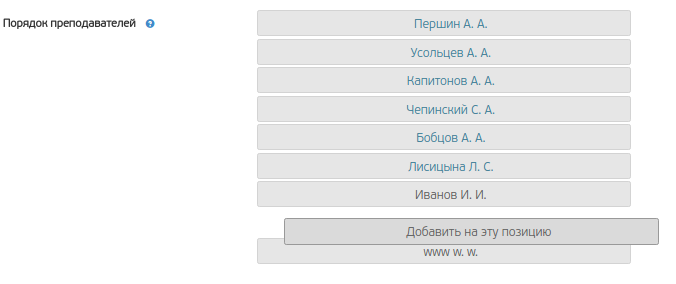
\includegraphics[width=0.8\linewidth]{create_instructors.png}}
		\caption{Изменение порядка преподавателей}
		\label{instructor:create_instructors}
		\end{figure}	
		
Видимость преподавателя на сайте настраивается путем переключения значения поля \quotes{Опубликован}. Неопубликованные преподаватели скрыты на сайте для пользователей. В форме в списке преподавателей показываются как скрытые, так и опубликованные преподаватели, в зависимости от статуса их ФИО имеют различный цвет. Подробное описание можно получить, нажав на иконку \vcenteredinclude[width=0.06\linewidth]{help_icon.png} рядом с меткой поля (см. рис.~\ref{instructor:create_instructors_legend}).
		
		\begin{figure}[H]
		\center{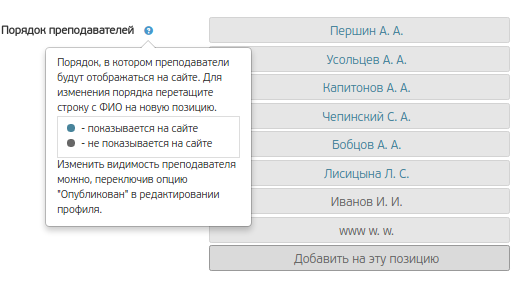
\includegraphics[width=1\linewidth]{create_instructors_legend.png}}
		\caption{Справка о статусе преподавателей}
		\label{instructor:create_instructors_legend}
		\end{figure}	

	\section{Курсы}
\subsection{Роли и операции}

Раздел доступен пользователям, имеющим следующие роли:

\begin{itemize}
	\item Администратор вуза"=поставщика:
	\begin{itemize}
		\item возможность просматривать курсы в данном университете;
		\item возможность создания/редактирования курса в данном университете;
		\item возможность назначения авторов курса при создании/редактировании курса.
	\end{itemize}
	\item Администратор контента вуза"=поставщика:
	\begin{itemize}
		\item возможность просматривать курсы в данном университете;
		\item возможность редактирования курса в данном университете.
	\end{itemize}
	\item Автор курса:
	\begin{itemize}
		\item возможность просматривать свой курс;
		\item возможность редактировать свой курс;
		\item возможность назначать авторов своего курса.
	\end{itemize}
	\item Администратор Платформы:
	\begin{itemize}
		\item просматривать курсы любого университета;
		\item создавать курс в любом университете;
		\item редактирование любого курса;
		\item назначение команды курса.
	\end{itemize}
\end{itemize}
\subsection{Список курсов}
\label{course:subsec:course_list}
В данном разделе находится список курсов (рис.~\ref{img:course:course_list}).

\begin{figure}[H]
	\center{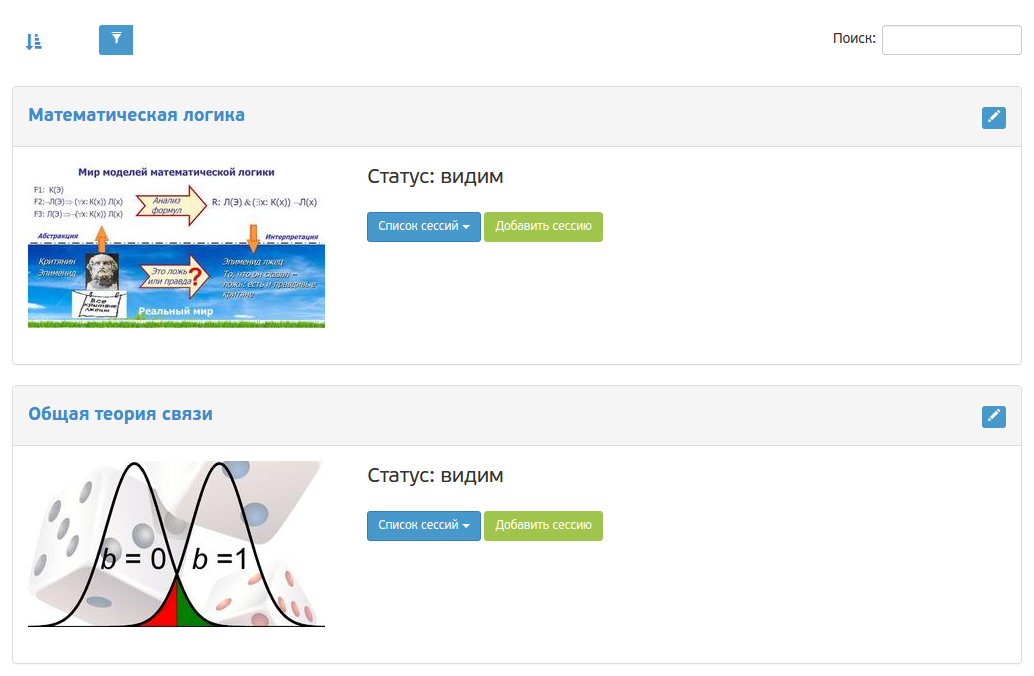
\includegraphics[width=1\linewidth]{images/course/course_list}}
	\caption{Внешний вид списка курсов.}
	\label{img:course:course_list}
\end{figure}

Каждый курс представлен отдельным элементом списка, на котором отображено:
\begin{itemize}
	\item Название курса. Если у пользователя есть право на просмотр данного курса, то при нажатии на название курса происходит переход на страницу подробной информации о курсе. Подробно форма детального просмотра курса описана в разделе~\ref{course:subsec:course_detail}).
	\item Если у пользователя есть право на редактирование данного курса, то пользователю доступна кнопка редактирования курса \vcenteredinclude[height=25px]{images/course/course_edit_btn}.
	\item Обложка курса.
	\item Статус курса (видим или скрыт).
	\item Если у курса есть сессии и пользователь имеет право на какое"=либо действие с сессиями данного курса, то ему доступна кнопка \quotes{список сессий}, при нажатии на которую пользователю становится доступна таблица со списком сессий данного курса (рис.~\ref{img:course:course_session_list}). При повторном нажатии на кнопку, таблица со списком сессий курса скрывается.
	\begin{figure}[H]
		\center{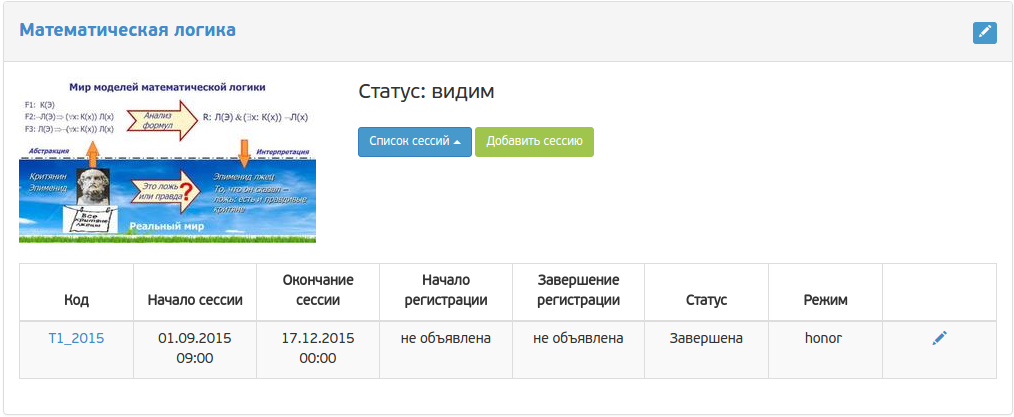
\includegraphics[width=1\linewidth]{images/course/course_session_list}}
		\caption{Список сессий курса}
		\label{img:course:course_session_list}
	\end{figure}
	
	\item Если у пользователя есть право на создание сессии, пользователю доступна кнопка \quotes{Добавить сессию}, при нажатии на которую пользователь переходит к окну создания сессии курса.
\end{itemize}

Единовременно на странице отображается не более 5 курсов. Если количество курсов больше пяти, происходит постраничное отображение курсов. Также на странице появляются элементы постраничной навигации (рис.~\ref{img:course:course_pagination}).

\begin{figure}[H]
	\center{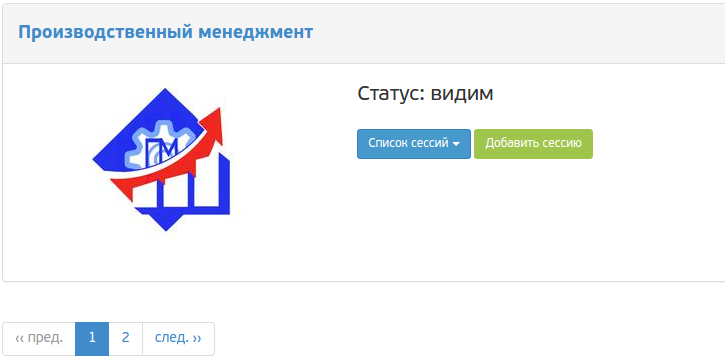
\includegraphics[width=1\linewidth]{images/course/course_pagination}}
	\caption{Элементы постраничной навигации при отображении курсов.}
	\label{img:course:course_pagination}
\end{figure}

Также имеется возможность упорядочить курсы в алфавитном порядке по возрастанию (убыванию) при помощи кнопки сортировки (рис.~\ref{img:course:course_filter_btn}).

\begin{figure}[H]
	\begin{minipage}[h]{0.49\linewidth}
		\center{
\includegraphics[width=0.1\linewidth]{images/course/course_sort_btn_az.png} \\ а)}
	\end{minipage}
	\hfill
	\begin{minipage}[h]{0.49\linewidth}
		\center{
\includegraphics[width=0.1\linewidth]{images/course/course_sort_btn_za.png} \\ б)}
	\end{minipage}
	\caption{a) сортировка по возрастанию, б) сортировка по убыванию}
	\label{img:course:course_filter_btn}
\end{figure}

Также возможен поиск среди курсов данного вуза по имени и статусу путем ввода текста в поле поиска \vcenteredinclude[height=25px]{images/datatables/search} (рис.~\ref{img:course:course_filter}).

\begin{figure}[H]
	\center{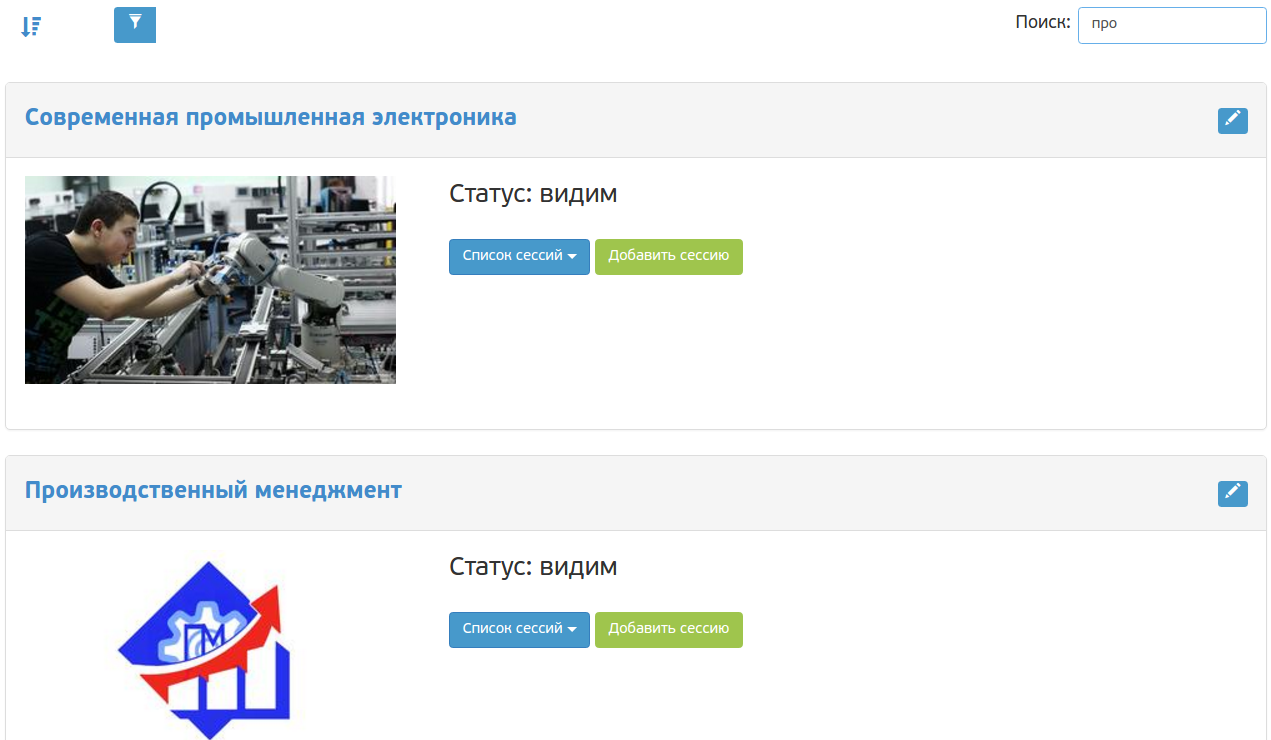
\includegraphics[width=1\linewidth]{images/course/course_filter}}
	\caption{Поиск курса по имени.}
	\label{img:course:course_filter}
\end{figure}

Возможна фильтрация курсов при помощи формы фильтрации, которая вызывается нажатием на кнопку фильтрации \vcenteredinclude[height=25px]{images/course/course_filter_form_btn}.

Форма фильтрации (рис.~\ref{img:course:course_filter_form}) позволяет фильтровать курсы по следующим параметрам:
\begin{itemize}
	\item название курса;
	\item статус курса (опубликован/скрыт);
	\item является ли данный курс рекомендованным (да/нет);
	\item находится ли данный курс в архиве (да/нет);
	\item преподаватель, который ведет курс (возможен выбор сразу нескольких см.\ раздел~\ref{widget:autocomplete_with_multiselect}).
\end{itemize}

\begin{figure}[H]
	\center{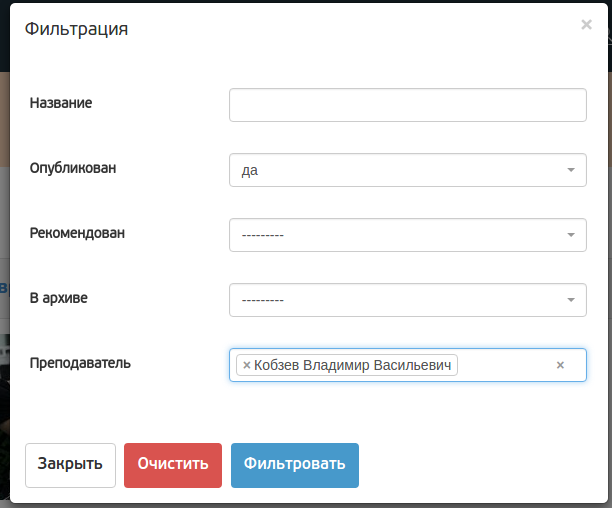
\includegraphics[width=1\linewidth]{images/course/course_filter_form}}
	\caption{Фильтр"=форма для списка курсов}
	\label{img:course:course_filter_form}
\end{figure}

При нажатии на кнопку \quotes{Фильтровать} происходит применение заданных пользователем фильтров. При нажатии на кнопку \quotes{Очистить} происходит очистка всех полей формы фильтрации. При нажатии на кнопку закрыть (или на крестик, или на область вне формы фильтрации), происходит закрытие формы фильтрации без применения фильтров.

Если применен хотя бы один фильтр, то рядом с кнопкой фильтрации появляется кнопка очистки формы фильтрации \vcenteredinclude[height=25px]{images/course/course_filter_form_btn_clear}.

Если у пользователя есть право на создание курса, то слева пользователю показывается кнопка
\vcenteredinclude[height=25px]{images/course/course_create_btn}, при нажатии на которую пользователь переходит на страницу создания курса.

Также, находясь в секции \quotes{Курсы}, пользователь в любой момент может перейти к списку курсов, нажав на кнопку \quotes{Список курсов}.

\subsection{Просмотра детальной информации о курсе}
\label{course:subsec:course_detail}
На данную страницу можно перейти, нажав на название курса на странице просмотра списка курсов, описанного в разделе~\ref{course:subsec:course_list}. Внешний вид страницы просмотра детальной информации о курсе представлен на рисунке~\ref{img:course:course_detail}.
\begin{figure}[H]
	\center{\includegraphics[width=1\linewidth]{images/course/course_detail}}
	\caption{Детальная информация о курсе}
	\label{img:course:course_detail}
\end{figure}

В верхней части данной страницы отображена обложка курса и его название. Если у пользователя есть право на редактирование данного курса, то в правом верхнем углу находится кнопка \vcenteredinclude[height=25px]{images/course/course_edit_btn}, нажатие на которую ведет к странице редактирования данного курса.

На странице отображается следующая информация о курсе:
\begin{itemize}
	\item обложка курса;
	\item название курса;
	\item код курса;
	\item промовидео;
	\item обложка промовидео;
	\item описание курса;
	\item о курсе;
	\item формат курса;
	\item ссылки на внешние ресурсы;
	\item результаты обучения;
	\item знания, навыки и умения, приобретаемые после прохождения курса;
	\item описание сертификата, который выдается по прохождении курса;
	\item значок сертификата;
	\item описание условий выдачи сертификата;
	\item компетенции образовательного стандарта;
	\item количество времени, которое нужно уделять для прохождения курса;
	\item количество зачетных единиц;
	\item опубликован ли данный курс;
	\item рекомендован ли данный курс;
	\item программа курса;
	\item требования к прохождению курса;
	\item дополнительная информация о курсе;
	\item дополнительная информация о курсе, которая будет размещена в правом блоке;
	\item список преподавателей, преподающих этот курс в порядке отображения на странице курса;
	\item список направлений подготовки, для которых предназначается этот курс;
	\item список групп дисциплин, для которых отображается данный курс;
	\item произвольные направления подготовки;
	\item список авторов курса.
\end{itemize}

\subsection{Создание/редактирование курса}
\label{course:subsec:course_create}
Форма создания/редактирования курса разбита на несколько блоков, для удобства заполнения:
\subsubsection{Основная информация}
	\begin{itemize}
		\item \textbf{Код курса} "--- уникальный (в рамках вуза) код курса. Должен иметь длину не более чем 25 символов, состоять из символов латинского алфавита верхнего и нижнего регистра. В случае, если курс с данным кодом существует в рамках данного университета, то внизу поля появится сообщение об ошибке (рис.~\ref{img:course:slug_error}). Обязательное поле. В режиме редактирования курса данное поле нельзя изменять.
		\begin{figure}[H]
			\center{\includegraphics[width=1\linewidth]{images/course/slug_error}}
			\caption{Ошибка, указывающая на то, что курс с таким кодом уже существует}
			\label{img:course:slug_error}
		\end{figure}
		\item \textbf{Название} курса "--- может состоять из любых символов и иметь длину до 200 символов. Обязательное поле.
		\item \textbf{Университет} "--- название университета, к которому принадлежит курс. Нередактируемое поле.
		\item \textbf{Опубликован} "--- переключатель, задающий видимость данного курса на странице курсов, доступных для прохождения.
		\item \textbf{Рекомендован} "--- переключатель, задающий, является ли данный курс рекомендованным к прохождению.
		\item \textbf{Преподаватели} "--- список преподавателей, которые ведут данный курс. Для того, чтобы добавить нового преподавателя, необходимо нажать на кнопку \quotes{Добавить} (рис.~\ref{img:course:instructor_list}), после чего выбрать нужного преподавателя из списка (в списке содержатся только преподаватели из данного вуза). Также осуществляется фильтрация по ФИО преподавателя (подробнее в подразделе~\ref{widget:autocomplete}). Для того, чтобы убрать преподавателя из списка, необходимо нажать на \quotes{крестик} рядом с именем преподавателя. Порядок преподавателей можно изменять с помощью перетаскивания (подробнее в подразделе~\ref{widget:ordering}). Порядок преподавателей задает порядок отображения преподавателей на странице курса.
		\begin{figure}[H]
			\center{\includegraphics[width=1\linewidth]{images/course/instructor_list}}
			\caption{Поле для формирования списка преподавателей курса}
			\label{img:course:instructor_list}
		\end{figure}		

		\item \textbf{Группы дисциплин} "--- список дисциплин, для которых предназначается данный курс. Для того, чтобы добавить новую группу, необходимо нажать на кнопку \quotes{Добавить}, после чего выбрать нужную группу из списка. Также осуществляется фильтрация по названию группы (подробнее в пункте~\ref{widget:autocomplete}). Для того, чтобы убрать группу из списка, необходимо нажать на \quotes{крестик} рядом с названием группы.
		\item \textbf{Направления подготовки} "--- список направлений подготовки, для которых предназначается данный курс. Для того, чтобы добавить новое направление, необходимо нажать на кнопку \quotes{Добавить}, после чего выбрать нужное направление из списка. Также осуществляется фильтрация по названию направления подготовки (подробнее в пункте~\ref{widget:autocomplete}). Для того, чтобы убрать направление из списка, необходимо нажать на \quotes{крестик} рядом с названием группы.
		\item \textbf{Произвольные направления подготовки} "--- текстовое поле.
		\item \textbf{Авторы курса} "--- список авторов курса.  Для того, чтобы добавить нового пользователя в список авторов курса, необходимо нажать на кнопку \quotes{Добавить}, после чего выбрать нужного пользователя из списка. Также осуществляется фильтрация по имени пользователя и по адресу электронной почты (подробнее в пункте~\ref{widget:autocomplete}). Для того, чтобы убрать пользователя из списка, необходимо нажать на \quotes{крестик} рядом с именем преподавателя.
		\item \textbf{Список сессий курса} "--- список сессий данного курса, представленный в виде таблицы  (рис.~\ref{img:course:course_session_table}).
		\begin{figure}[H]
			\center{\includegraphics[width=1\linewidth]{images/course/course_session_table}}
			\caption{Таблица со списком сессий курса}
			\label{img:course:course_session_table}
		\end{figure}
		
		Таблица со списком сессий курса имеет следующие столбцы:
		\begin{itemize}
			\item \textbf{Код} "--- код сессии курса. При щелчке на код сессии, происходит переход на детальное отображение данной сессии курса (подробнее про отображение детальной информации о сессии курса описано в разделе~\ref{course_session:course_session_detail}.
			\item \textbf{Начало сессии} "--- дата начала сессии курса. В случае, если дата начала сессии курса не задана, отображается надпись \quotes{не объявлена}.
			\item \textbf{Окончание сессии} "--- дата окончания сессии курса. В случае, если дата окончания сессии курса не задана, отображается надпись \quotes{не объявлена}.
			\item \textbf{Начало регистрации} "--- дата начала регистрации на сессию курса. В случае, если дата начала регистрации не задана, отображается надпись \quotes{не объявлена}.
			\item \textbf{Завершение регистрации} "--- дата завершения регистрации на сессию курса. В случае, если дата завершения регистрации не задана, отображается надпись \quotes{не объявлена}.
			\item \textbf{Статус} "--- статус сессии курса.
			\item \textbf{Режим} "--- список возможных режимов прохождения сессии курса.
			\item Кнопка редактирования сессии курса \vcenteredinclude[height=25px]{images/course_session/session_edit_btn} "--- переводит пользователя на страницу редактирования данной сессии курса (отображается если у пользователя есть право на редактирование сессии курса).
		\end{itemize}
	\end{itemize}
\subsubsection{Дополнительная информация}
	\begin{itemize}
		\item \textbf{Описание} "--- текстовое поле, содержащее в себе краткое описание курса. Допускает HTML"=разметку (работа с данным полем описана в пункте~\ref{widget:ckeditor}).
		\item \textbf{О курсе} "--- текстовое поле, содержащее в себе описание курса.  Допускает HTML"=разметку (работа с данным полем описана в пункте~\ref{widget:ckeditor}). Если курс опубликован, то данное поле является обязательным и в нем должно быть записано не менее 200 значащих символов (символы латинского, русского алфавита, цифры и т.д.). В противном случае данное поле необязательно.
		\item \textbf{Формат курса} "--- текстовое поле, содержащее в себе описание формата курса. Допускает HTML"=разметку (работа с данным полем описана в пункте~\ref{widget:ckeditor}).
		\item \textbf{Внешние ресурсы} "--- текстовое поле, содержащее в себе ссылки на внешние ресурсы, которые могут помочь в освоении курса. Допускает HTML"=разметку (работа с данным полем описана в пункте~\ref{widget:ckeditor}).
		\item \textbf{Программа курса} "--- текстовое поле, содержащее в себе описание программы курса.Допускает HTML"=разметку (работа с данным полем описана в пункте~\ref{widget:ckeditor}).
		\item \textbf{Требования} "--- текстовое поле, содержащее в себе описание требований курса. Допускает HTML"=разметку (работа с данным полем описана в пункте~\ref{widget:ckeditor}).
		\item \textbf{Дополнительная информация} "--- текстовое поле, содержащее в себе дополнительную информацию о курсе. Допускает HTML"=разметку (работа с данным полем описана в пункте~\ref{widget:ckeditor}).
		\item \textbf{Дополнительная информация в правом блоке} "--- текстовое поле, содержащее в себе описание дополнительной информации, которая будет выводиться в правом блоке на странице просмотра курса. Допускает HTML"=разметку (работа с данным полем описана в пункте~\ref{widget:ckeditor}).
	\end{itemize}
\subsubsection{Результаты обучения}
	\begin{itemize}
		\item \textbf{Результаты обучения} "--- текстовое поле, содержащее в себе результаты прохождения курса. Допускает HTML"=разметку (работа с данным полем описана в пункте~\ref{widget:ckeditor}).
		\item \textbf{Знания} "--- текстовое поле, содержащее в себе описание знаний, которые человек получит в процессе прохождения курса. Допускает HTML"=разметку (работа с данным полем описана в пункте~\ref{widget:ckeditor}).
		\item \textbf{Навыки} "--- текстовое поле, содержащее в себе описание навыков, которые человек получит в процессе прохождения курса. Допускает HTML"=разметку (работа с данным полем описана в пункте~\ref{widget:ckeditor}).
		\item \textbf{Умения} "--- текстовое поле, содержащее в себе описание умений, которые человек получит в процессе прохождения курса. Допускает HTML"=разметку (работа с данным полем описана в пункте~\ref{widget:ckeditor}).
	\end{itemize}
\subsubsection{Нагрузка}
	\begin{itemize}
		\item \textbf{Часов в неделю от} "--- минимальная нагрузка в неделю. Может принимать значение от 1 до 40. Если указана максимальная нагрузка, то необходимо указать минимальную, при этом минимальная нагрузка не должна быть больше максимальной.
		\item \textbf{Часов в неделю до} "--- максимальная нагрузка в неделю. Может принимать значение от 1 до 40. Если указана минимальная нагрузка, то необходимо указать максимальную, при этом максимальная нагрузка не должна быть меньше минимальной.
		\item \textbf{Зачётных единиц} "--- количество зачетных единиц, которые необходимо сдать для успешного завершения курса. Может принимать значение от 1 до 10.
		\item \textbf{Длительность (недель)} "--- продолжительность (в неделях) курса. Может принимать значение от 1 до 16.
	\end{itemize}
\subsubsection{Медиа}
	\begin{itemize}
		\item \textbf{Обложка} "--- обложка курса, отображаемая пользователю. Ширина и высота загружаемого изображения не должны превышать 600 пикселей, а размер изображения не должен быть больше 1 Мб.
		Возможно загружать изображения в следующих форматах: png, jpg, jpeg, gif. Процесс загрузки изображения описан в пункте~\ref{widget:file_upload}.
		\item \textbf{Промовидео} "--- ссылка на промовидео курса.
		\item \textbf{Картинка для видео} "--- обложка для промовидео. Ширина и высота загружаемого изображения не должны превышать 600 пикселей, а размер изображения не должен быть больше 1 Мб. Возможно загружать изображения в следующих форматах: png, jpg, jpeg, gif. Процесс загрузки изображения описан в пункте~\ref{widget:file_upload}.
	\end{itemize}
\subsubsection{Информация о сертификате}
	\begin{itemize}
		\item \textbf{Сертификат} "--- текстовое поле, содержащее в себе описание выдаваемого сертификата, которые человек получит после прохождения курса. Допускает HTML"=разметку  (работа с данным полем описана в пункте~\ref{widget:ckeditor}).
		\item \textbf{Компетенции образовательного стандарта} "--- текстовое поле, содержащее в себе описание компетенции образовательного стандарта. Допускает HTML"=разметку (работа с данным полем описана в пункте~\ref{widget:ckeditor}).
		\item \textbf{Значок сертификата} "--- обложка для промовидео. Ширина и высота загружаемого изображения не должны превышать 600 пикселей, а размер изображения не должен быть больше 1 Мб. Возможно загружать изображения в следующих форматах: png, jpg, jpeg, gif. Процесс загрузки изображения описан в пункте~\ref{widget:file_upload}.
		\item \textbf{Описание условий выдачи сертификата} "--- текстовое поле, содержащее в себе описание условий выдачи сертификата о прохождении курса. Допускает HTML"=разметку (работа с данным полем описана в пункте~\ref{widget:ckeditor}).
	\end{itemize}
\subsubsection{Элементы управления}
	\begin{itemize}
		\item \vcenteredinclude[height=25px]{images/course/form_cancel_btn} "--- кнопка отмены сохранения формы. При нажатии на данную кнопку пользователь будет перенаправлен предыдущую страницу.
		\item \vcenteredinclude[height=25px]{images/course/form_view_btn} "--- кнопка предпросмотра курса. При нажатии на данную кнопку пользователю будет показано, как курс будет отображаться пользователям. Закрытие модального окна производится нажатием на крестик в верхнем правом углу окна или щелчком за пределами данного окна.
		\begin{figure}[H]
			\center{\includegraphics[width=1\linewidth]{images/course/course_preview}}
			\caption{Пример предпросмотра курса}
			\label{img:course:course_preview}
		\end{figure}
		
		\item \vcenteredinclude[height=25px]{images/course/form_save_btn} "--- кнопка сохранения курса. Если параметры курса заданы корректно, то при нажатии на кнопку будет произведено сохранение курса, а пользователь будет перенаправлен на страницу списка курсов. В противном случае будет произведена прокрутка до первого поля, в котором обнаружена ошибка.
	\end{itemize}
	\section{Сессия курса}

Ниже перечислены роли, имеющие доступ к данному разделу и их права,
в рамках данного раздела.

\subsection{Роли и операции}
Раздел доступен пользователям, имеющим следующие роли:
\begin{itemize}
	\item Администратор вуза"=поставщика:
	\begin{itemize}
		\item возможность просматривать сессии в данном университете;
		\item возможность создания/редактирования сессии курса в данном университете;
		\item возможность назначения команды сессии курса при создании/редактировании сессии курса.
	\end{itemize}
	\item Администратор контента вуза"=поставщика:
	\begin{itemize}
		\item возможность просматривать сессии курсов в данном университете;
		\item возможность редактирования сессий курсов в данном университете.
	\end{itemize}
	\item Автор курса:
	\begin{itemize}
		\item возможность просматривать сессии своего курса;
		\item возможность создавать сессии для своего курса;
		\item возможность редактировать сессии своего курса;
		\item возможность назначать команду сессии курса.
	\end{itemize}
	\item Администратор Платформы:
	\begin{itemize}
		\item возможность просмотра сессию курсов любого курса;
		\item возможность создания сессию курса для любого курса;
		\item возможность редактирования любой сессии курса;
		\item возможность назначения команды любой сессии курса.
	\end{itemize}
\end{itemize}
\subsection{Список сессий курсов}
\label{course_session:course_session_list}
	Список сессий курса для каждого курса перечислен в таблице после каждого курса (рис.~\ref{img:course_session:course_session_table}).
	\begin{figure}[H]
		\center{\includegraphics[width=1\linewidth]{images/course_session/course_session_table}}
		\caption{Таблица со списком сессий курса.}
		\label{img:course_session:course_session_table}
	\end{figure}
	
	Для того, чтобы отобразить/скрыть таблицу со списком сессий курса необходимо нажать на кнопку \vcenteredinclude[height=25px]{images/course_session/session_list_btn}. В случае, если у курса отсутствуют сессии, то на месте кнопки \quotes{Список сессий} будет надпись \quotes{Нет сессий} (рис.~\ref{img:course_session:course_without_sessions}).
		\begin{figure}[H]
			\center{\includegraphics[width=0.4\linewidth]{images/course_session/course_without_sessions}}
			\caption{Сообщение в случае отсутствия сессий курса}
			\label{img:course_session:course_without_sessions}
		\end{figure}
		
	Таблица со списком сессий курса имеет следующие столбцы:
	\begin{itemize}
		\item \textbf{Код} "--- код сессии курса. При щелчке на код сессии, происходит переход на детальное отображение данной сессии курса (см.\ раздел~\ref{course_session:course_session_detail}.
		\item \textbf{Начало сессии} "--- дата начала сессии курса. В случае, если дата начала сессии курса не задана, отображается надпись \quotes{не объявлена}.
		\item \textbf{Окончание сессии} "--- дата окончания сессии курса. В случае, если дата окончания сессии курса не задана, отображается надпись \quotes{не объявлена}.
		\item \textbf{Начало регистрации} "--- дата начала регистрации на сессию курса. В случае, если дата начала регистрации не задана, отображается надпись \quotes{не объявлена}.
		\item \textbf{Завершение регистрации} "--- дата завершения регистрации на сессию курса. В случае, если дата завершения регистрации не задана, отображается надпись \quotes{не объявлена}.
		\item \textbf{Статус} "--- статус сессии курса.
		\item \textbf{Режим} "--- список возможных режимов прохождения сессии курса.
		\item Кнопка редактирования сессии курса \vcenteredinclude[height=25px]{images/course_session/session_edit_btn} "--- переводит пользователя на страницу редактирования данной сессии курса (отображается если у пользователя есть право на редактирование сессии курса).
	\end{itemize}
	
	Для создания новой сессии курса необходимо нажать на кнопку \vcenteredinclude[height=25px]{images/course_session/session_create_btn} (отображается если у пользователя есть право создать сессию курса), после чего пользователя перенаправит на страницу создания новой сессии курса.

\subsection{Просмотр детальной информации о сессии курса}
\label{course_session:course_session_detail}
	Переход на данную страницу осуществляется путем нажатия на код сессии курса в таблице сессий курса (пункт~\ref{course_session:course_session_list}). Внешний вид страницы представлен на рисунке~\ref{img:course_session:course_sessions_detail}.
	
	\begin{figure}[H]
		\center{\includegraphics[width=1\linewidth]{images/course_session/course_session_detail}}
		\caption{Детальная информация о сессии курса}
		\label{img:course_session:course_sessions_detail}
	\end{figure}
	
	В верхней части данной страницы отображен код сессии курса. Если у пользователя есть право на редактирование данной сессии курса, то в правом верхнем углу находится кнопка \vcenteredinclude[height=25px]{images/course/course_edit_btn}, нажатие на которую ведет к странице редактирования данной сессии курса. Для удобства отображения, вся информация о сессии курса разнесена на несколько частей, переключение между которыми происходит при помощи закладок (рис.~\ref{img:course_session:course_sessions_tabs}).
	\begin{figure}[H]
		\center{\includegraphics[width=1\linewidth]{images/course_session/course_session_tabs}}
		\caption{Закладки на странице детальной информации о сессии курса}
		\label{img:course_session:course_sessions_tabs}
	\end{figure}
	
	В закладке \quotes{Основная информация} отображается следующая информация о сессии курса:
	\begin{itemize}
		\item ссылка на курс, к которому принадлежит данная сессия;
		\item внешняя ссылка на курс;
		\item время прохождения сессии курса;
		\item время записи на сессию курса;
		\item период предоставления доступа к материалам сессии курса;
		\item период отображения слушателям;
		\item необходимо ли принятие Honor Code;
		\item были ли отправлены письма, уведомляющие о начале курса;
		\item формат курса;
		\item ссылки на внешние ресурсы;
		\item результаты обучения;
		\item знания, навыки и умения, приобретаемые после прохождения курса;
		\item описание сертификата, который выдается по прохождению курса;
		\item значок сертификата;
		\item описание условий выдачи сертификата;
		\item компетенции образовательного стандарта;
		\item программа курса;
		\item количество времени, которое нужно уделять для прохождения сессии курса;
		\item количество зачетных единиц;
		\item требования к прохождению сессии курса;
		\item дополнительная информация о сессии курса;
		\item дополнительная информация о сессии курса, которая будет размещена в правом блоке;
		\item список преподавателей, преподающих эту сессию курса в порядке отображения на странице курса;
		\item команда курса. 
	\end{itemize}
	
	В остальных закладках отображена информация о соответствующих режимах прохождения сессии курса, а именно:
	\begin{itemize}
		\item активен ли данный режим прохождения;
		\item период приема оплаты данного режима;
		\item стоимость;
		\item кратное описание режима прохождения;
		\item подробное описание режима прохождения;
		\item сертификат, выдаваемый после завершения данного режима.
	\end{itemize}

\subsection{Создание/редактирование сессии курса}
Форма создания/редактирования сессии курса разбита на несколько блоков, для удобства заполнения:
	\subsubsection{Основная информация}
	\begin{itemize}
		\item \textbf{Код сессии} "--- должен иметь длину не более чем 25 символов, состоять из символов латинского алфавита верхнего и нижнего регистра, а также быть уникальным в рамках курса. В случае, если сессия курса с данным кодом существует в рамках данного курса, то внизу поля появится сообщение об ошибке (рис.~\ref{img:course_session:slug_error}). Обязательное поле. В режиме редактирования сессии курса данное поле нельзя изменять.
		\begin{figure}[H]
			\center{\includegraphics[width=1\linewidth]{images/course_session/slug_error}}
			\caption{Ошибка, указывающая на то, что сессия курса с таким кодом уже существует.}
			\label{img:course_session:slug_error}
		\end{figure}
		
		\item \textbf{Курс} "--- код и название курса, к которому принадлежит сессия курса. Нередактируемое поле.
		\item \textbf{Дата и время начала сессии курса} "--- дата и время начала сессии курса. Не может быть больше значения поля \quotes{Дата и время окончания сессии курса}, если оно задано. Дата и время задается в формате \quotes{ДД.ММ.ГГГГ ЧЧ.мм}. Для более удобного задания даты, можно воспользоваться виджетом задания даты и времени, описанном в разделе~\ref{widget:date_time_picker}.
		
		\item \textbf{Дата и время окончания сессии курса} "--- дата и время окончания сессии курса. Не может быть меньше значения поля \quotes{Дата и время начала сессии курса}, если оно задано. Дата и время задается в формате \quotes{ДД.ММ.ГГГГ ЧЧ.мм}. Для более удобного задания даты, можно воспользоваться виджетом задания даты и времени, описанном в разделе~\ref{widget:date_time_picker}.
		
		\item \textbf{Дата и время открытия записи на сессию курса} "--- дата и время начала записи на сессию курса. Не может быть больше значения поля \quotes{Дата и время закрытия записи на сессию курса}, если оно задано. Дата и время задается в формате \quotes{ДД.ММ.ГГГГ ЧЧ.мм}. Для более удобного задания даты, можно воспользоваться виджетом задания даты и времени, описанном в разделе~\ref{widget:date_time_picker}.
		
		\item \textbf{Дата и время закрытия записи на сессию курса} "--- дата и время окончания записи на сессию курса. Не может быть меньше значения поля \quotes{Дата и время открытия записи на сессию курса}, если оно задано. Дата и время задается в формате \quotes{ДД.ММ.ГГГГ ЧЧ.мм}. Для более удобного задания даты, можно воспользоваться виджетом задания даты и времени, описанном в разделе~\ref{widget:date_time_picker}.
		
		\item \textbf{Преподаватели} "--- список преподавателей, которые ведут данную сессию курса. Для того, чтобы добавить нового преподавателя, необходимо нажать на кнопку \quotes{Добавить} (рис.~\ref{img:course_session:instructor_list}), после чего выбрать нужного преподавателя из списка (в списке содержатся только преподаватели из данного вуза). Также осуществляется фильтрация по ФИО преподавателя (подробнее в пункте~\ref{widget:autocomplete}). Для того, чтобы убрать преподавателя из списка, необходимо нажать на \quotes{крестик} рядом с именем преподавателя. Порядок преподавателей можно изменять (подробнее в пункте~\ref{widget:ordering}) (рис.~\ref{img:course_session:instructor_sort}, перетаскивая элементы списка (порядок преподавателей задает порядок отображения преподавателей на странице курса).
		\begin{figure}[H]
			\center{\includegraphics[width=1\linewidth]{images/course/instructor_list}}
			\caption{Поле задания преподавателей сессии курса.}
			\label{img:course_session:instructor_list}
		\end{figure}		
		\begin{figure}[H]
			\center{\includegraphics[width=1\linewidth]{images/course/instructor_sort}}
			\caption{Изменение порядка преподавателей сессии курса.}
			\label{img:course_session:instructor_sort}
		\end{figure}
		При создании сессии курса данное поле заполняется данными поля \quotes{Преподаватели} соответствующего курса.
	\end{itemize}

\subsubsection{Дополнительная информация}
	\begin{itemize}
		\item \textbf{Формат сессии курса} "--- текстовое поле, содержащее в себе описание формата сессии курса. Допускает HTML"=разметку (работа с данным полем описана в пункте~\ref{widget:ckeditor}).
		При создании сессии курса данное поле заполняется данными поля \quotes{Формат курса} соответствующего курса.
		
		\item \textbf{Внешние ресурсы} "--- текстовое поле, содержащее в себе ссылки на внешние ресурсы, которые могут помочь в прохождении сессии курса. Допускает HTML"=разметку (работа с данным полем описана в пункте~\ref{widget:ckeditor}). При создании сессии курса данное поле заполняется данными поля \quotes{Внешние ресурсы} соответствующего курса.
		
		\item \textbf{Программа сессии курса} "--- текстовое поле, содержащее в себе описание программы сессии курса. Допускает HTML"=разметку (работа с данным полем описана в пункте~\ref{widget:ckeditor}). При создании сессии курса данное поле заполняется данными поля \quotes{Программа курса} соответствующего курса.
		
		\item \textbf{Требования} "--- текстовое поле, содержащее в себе описание требований сессии курса. Допускает HTML"=разметку (работа с данным полем описана в пункте~\ref{widget:ckeditor}). При создании сессии курса данное поле заполняется данными поля \quotes{Требования} соответствующего курса.
		
		\item \textbf{Внешняя ссылка на курс} "--- внешняя ссылка на курс, к которому принадлежит текущая сессия курса. Должно содержать в себе URL на страницу курса. При неправильном адресе (введен невалидный URL), пользователю будет показано сообщение, приведённое на рис.~\ref{img:course_session:url-error}.
		\begin{figure}[H]
			\center{\includegraphics[width=1\linewidth]{images/course_session/url-error}}
			\caption{Пример отображения сообщения об ошибке при заполнении поля \quotes{Внешняя ссылка на курс}.}
			\label{img:course_session:url-error}
		\end{figure}
		
		\item \textbf{Дополнительная информация} "--- текстовое поле, содержащее в себе дополнительную информацию о сессии курса. Допускает HTML"=разметку (работа с данным полем описана в пункте~\ref{widget:ckeditor}). При создании сессии курса данное поле заполняется данными поля \quotes{Дополнительная информация} соответствующего курса.
		
		\item \textbf{Дополнительная информация в правом блоке} "--- текстовое поле, содержащее в себе описание дополнительной информации, которая будет выводиться в правом блоке на странице просмотра курса. Допускает HTML"=разметку (работа с данным полем описана в пункте~\ref{widget:ckeditor}). При создании сессии курса данное поле заполняется данными поля \quotes{Дополнительная информация в правом блоке} соответствующего курса.
	\end{itemize}

\subsubsection{Результаты обучения}
	\begin{itemize}
		\item \textbf{Результаты обучения} "--- текстовое поле, содержащее в себе результаты прохождения сессии курса. Допускает HTML"=разметку (работа с данным полем описана в пункте~\ref{widget:ckeditor}). При создании сессии курса данное поле заполняется данными поля \quotes{Дополнительная информация в правом блоке} соответствующего курса.
		
		\item \textbf{Знания} "--- текстовое поле, содержащее в себе описание знаний, которые человек получит в процессе прохождения сессии курса. Допускает HTML"=разметку (работа с данным полем описана в пункте~\ref{widget:ckeditor}). При создании сессии курса данное поле заполняется данными поля \quotes{Знания} соответствующего курса.
		
		\item \textbf{Навыки} "--- текстовое поле, содержащее в себе описание навыков, которые человек получит в процессе прохождения сессии курса. Допускает HTML"=разметку (работа с данным полем описана в пункте~\ref{widget:ckeditor}). При создании сессии курса данное поле заполняется данными поля \quotes{Навыки} соответствующего курса.
		
		\item \textbf{Умения} "--- текстовое поле, содержащее в себе описание умений, которые человек получит в процессе прохождения сессии курса. Допускает HTML"=разметку (работа с данным полем описана в пункте~\ref{widget:ckeditor}). При создании сессии курса данное поле заполняется данными поля \quotes{Умения} соответствующего курса.
	\end{itemize}

\subsubsection{Доступ}
	\begin{itemize}
		\item \textbf{Дата и время предоставления доступа к материалам сессии курса} "--- дата начала предоставления доступа к материалам сессии курса. Значение данного поля не должно быть больше значения поля \quotes{Дата и время прекращения доступа к материалам сессии курса}, если оно задано. Дата и время задается в формате \quotes{ДД.ММ.ГГГГ ЧЧ.мм}. Для более удобного задания даты, можно воспользоваться виджетом задания даты и времени, описанном в разделе~\ref{widget:date_time_picker}.
		
		\item \textbf{Дата и время прекращения доступа к материалам сессии курса} "--- дата окончания предоставления доступа к материалам сессии курса. Значение данного поля не должно быть меньше значения поля \quotes{Дата и время предоставления доступа к материалам сессии курса}, если оно задано. Дата и время задается в формате \quotes{ДД.ММ.ГГГГ ЧЧ.мм}. Для более удобного задания даты, можно воспользоваться виджетом задания даты и времени, описанном в разделе~\ref{widget:date_time_picker}.
		
		\item \textbf{Дата начала для отображения слушателям} "--- дата начала отображения сессии курса. Значение данного поля не должно быть больше значения поля \quotes{Дата окончания для отображения слушателям}, если оно задано. Дата и время задается в формате \quotes{ДД.ММ.ГГГГ ЧЧ.мм}. Для более удобного задания даты, можно воспользоваться виджетом задания даты и времени, описанном в разделе~\ref{widget:date_time_picker}.
		
		\item \textbf{Дата окончания для отображения слушателям} "--- дата окончания отображения сессии курса. Значение данного поля не должно быть меньше значения поля \quotes{Дата начала для отображения слушателям}, если оно задано. Дата и время задается в формате \quotes{ДД.ММ.ГГГГ ЧЧ.мм}. Для более удобного задания даты, можно воспользоваться виджетом задания даты и времени, описанном в разделе~\ref{widget:date_time_picker}.
	\end{itemize}
	
\subsubsection{Информация о сертификате}
	\begin{itemize}
		\item \textbf{Разрешен выпуск неподтвержденных сертификатов} "--- поле, задающее разрешен ли выпуск неподтвержденных сертификатов.
		
		\item \textbf{Сертификат} "--- текстовое поле, содержащее в себе описание выдаваемого сертификата, которые человек получит после прохождения курса. Допускает HTML"=разметку (работа с данным полем описана в пункте~\ref{widget:ckeditor}). При создании сессии курса данное поле заполняется данными поля \quotes{Сертификат} соответствующего курса.
		
		\item \textbf{Компетенции образовательного стандарта} "--- текстовое поле, содержащее в себе описание компетенции образовательного стандарта. Допускает HTML"=разметку (работа с данным полем описана в пункте~\ref{widget:ckeditor}). При создании сессии курса данное поле заполняется данными поля \quotes{Компетенции образовательного стандарта} соответствующего курса.
		
		\item \textbf{Значок сертификата} "--- обложка для промовидео. Ширина и высота загружаемого изображения не должны превышать 600 пикселей, а размер изображения не должен быть больше 1Мб.
		Возможно загружать изображения в следующих форматах: png, jpg, jpeg, gif. Процесс загрузки изображения описан в пункте~\ref{widget:file_upload}. При создании сессии курса данное поле заполняется данными поля \quotes{Значок сертификата} соответствующего курса.
		
		\item \textbf{Описание условий выдачи сертификата} "--- текстовое поле, содержащее в себе описание условий выдачи сертификата о прохождении курса. Допускает HTML"=разметку (работа с данным полем описана в пункте~\ref{widget:ckeditor}). При создании сессии курса данное поле заполняется данными поля \quotes{Описание условий выдачи сертификата} соответствующего курса.
	\end{itemize}
	
\subsubsection{Нагрузка}
	\begin{itemize}
		\item \textbf{Часов в неделю от} "--- минимальная нагрузка в неделю. Может принимать значение от 1 до 40. Если указана максимальная нагрузка, то необходимо указать минимальную, при этом минимальная нагрузка не должна быть больше максимальной. При создании сессии курса данное поле заполняется данными поля \quotes{Часов в неделю от} соответствующего курса.
		
		\item \textbf{Часов в неделю до} "--- максимальная нагрузка в неделю. Может принимать значение от 1 до 40. Если указана минимальная нагрузка, то необходимо указать максимальную, при этом максимальная нагрузка не должна быть меньше минимальной. При создании сессии курса данное поле заполняется данными поля \quotes{Часов в неделю до} соответствующего курса.
		
		\item \textbf{Зачётных единиц} "--- количество зачетных единиц, которые необходимо сдать для успешного завершения сессии курса. Может принимать значение от 1 до 10. При создании сессии курса данное поле заполняется данными поля \quotes{Зачётных единиц} соответствующего курса.
		
		\item \textbf{Длительность (недель)} "--- продолжительность (в неделях) сессии курса. Может принимать значение от 1 до 16. При создании сессии курса данное поле заполняется данными поля \quotes{Длительность} соответствующего курса.
	\end{itemize}
	
\subsubsection{Команда сессии курса}
	В данном разделе формы создания/редактирования сессии курса возможно назначение команды сессии курса: авторов сессии курса, членов команды курса и т.д. (при создании новой сессии курса, авторы сессии курса автоматически назначаются из авторов курса). Роли, назначенные пользователю, определяют набор действий, которые доступны пользователю. Для того, чтобы добавить нового члена команды сессии курса, необходимо нажать на кнопку \vcenteredinclude[height=25px]{images/course_session/course_session_team_add_btn}. После чего появится форма для добавления нового участника команды сессии курса (рис.~\ref{img:course_session:new_member}).
	\begin{figure}[H]
		\center{\includegraphics[width=1\linewidth]{images/course_session/course_session_team_new_member}}
		\caption{Добавление нового участника команды сессии курса}
		\label{img:course_session:new_member}
	\end{figure}
	Для корректного заполнения команды сессии курса необходимо выбрать пользователя и назначить ему как минимум одну роль. В противном случае будет показана ошибка, сообщающая о том, что данное поле обязательно (рис.~\ref{img:course_session:course_session_team_error}).
	\begin{figure}[H]
		\center{\includegraphics[width=1\linewidth]{images/course_session/course_session_team_error}}
		\caption{Пример некорректно заполненной строки с членом курса.}
		\label{img:course_session:course_session_team_error}
	\end{figure}
	
	Для удаления пользователя из команды сессии курса необходимо нажать на кнопку \vcenteredinclude[height=25px]{images/course_session/course_team_delete_btn}.
	
	Для более удобного поиска пользователя предусмотрен поиск по имени, фамилии и адресу электронной почты пользователя (подробнее работы с данным полем описана в разделе~\ref{widget:autocomplete}).
	
	При назначении ролей так же предусмотрен поиск нужной роли по её названию (подробнее работы с данным полем описана в разделе~\ref{widget:autocomplete_with_multiselect}).
	Одному пользователю можно назначить несколько ролей.
	
\subsubsection{Режимы прохождения}
	Каждой сессии можно назначить от 1 до 3 режимов прохождения сессии. Для каждой сессии курса может быть назначены следующие режимы прохождения:
	\begin{itemize}
		\item honor;
		\item audit;
		\item verified.
	\end{itemize}
	Режим honor является обязательным режимом для любой сессии курса, остальные режимы могут быть добавлены или убраны по желанию пользователя. Добавления нового режима прохождения осуществляется нажатием кнопки \vcenteredinclude[height=25px]{images/course_session/course_session_mode_add_btn} (так как у одной сессии не может быть больше трёх режимов прохождения, после добавления третьего режима прохождения, кнопка \quotes{Добавить режим} скрывается). Удаление режима прохождения сессии осуществляется нажатием кнопки \vcenteredinclude[height=25px]{images/course_session/course_team_delete_btn} (так как режим honor обязательный, кнопка, удаляющая элемент с данным режимом недоступна).
	
	Форма с каждым из режимов прохождения сессии курса содержит следующие поля:
	\begin{itemize}
		\item \textbf{Активен} "--- поле, задающее активен ли данный режим прохождения.
		
		\item \textbf{Тип} "--- поле, задающее тип режима прохождения. Можно выбрать не заданные для данной сессии курса режимы (так как режим honor обязателен, то данное поле в форме режима honor сделана неактивной).
		
		\item \textbf{Начало приема оплаты} "--- дата начала приема оплаты для данного режима (обязательно в режиме прохождения verified). Значение данного поля не должно быть больше значения поля \quotes{Крайняя дата оплаты} для данного режима прохождения (если оно задано). Дата и время задается в формате \quotes{ДД.ММ.ГГГГ ЧЧ.мм}. Для более удобного задания даты, можно воспользоваться виджетом задания даты и времени, описанном в разделе~\ref{widget:date_time_picker}.
		
		\item \textbf{Крайняя дата оплаты} "--- дата окончания приема оплаты для данного режима (обязательно в режиме прохождения verified). Значение данного поля не должно быть меньше значения поля \quotes{Начало приема оплаты} для данного режима прохождения (если оно задано). Дата и время задается в формате \quotes{ДД.ММ.ГГГГ ЧЧ.мм}. Для более удобного задания даты, можно воспользоваться виджетом задания даты и времени, описанном в разделе~\ref{widget:date_time_picker}.
		
		\item \textbf{Стоимость} "--- стоимость прохождения данного режима. Обязательное поле. В режиме verified стоимость должна быть больше 0, в противном случае будет выведено сообщение об ошибке (рис.~\ref{img:course_session:course_session_mode_cost_error}).
		\begin{figure}[H]
			\center{\includegraphics[width=1\linewidth]{images/course_session/course_session_mode_cost_error}}
			\caption{Пример сообщения об ошибке при неправильно заданной стоимости.}
			\label{img:course_session:course_session_mode_cost_error}
		\end{figure}
		
		\item \textbf{Краткое описание} "--- текстовое поле, в котором задается краткое описание режима прохождения сессии.
		
		\item \textbf{Описание} "--- текстовое поле, в котором задается полное описание режима прохождения сессии.
		
		\item \textbf{Сертификат} "--- сертификат, выдаваемый после прохождения режима прохождения сессии. Максимальный размер загружаемого файла "--- 20 Мб. Доступные форматы: png, jpg, jpeg, gif, txt, pdf, doc, docx, odt, html. Подробнее процесс загрузки файлов описан в пункте~\ref{widget:file_upload}.
	\end{itemize}
	
\subsubsection{Элементы управления}
\begin{itemize}
	\item \vcenteredinclude[height=25px]{images/course/form_cancel_btn} "--- кнопка отмены сохранения формы. При нажатии на данную кнопку пользователь будет перенаправлен предыдущую страницу.
	\item \vcenteredinclude[height=25px]{images/course/form_view_btn} "--- кнопка предпросмотра сессии курса. При нажатии на данную кнопку пользователю будет показано, как курс будет отображаться пользователям при условии, что редактируемая (создаваемая) сессия является активной. Закрытие модального окна производится нажатием на крестик в верхнем правом углу окна или щелчком за пределами данного окна.
	\begin{figure}[H]
		\center{\includegraphics[width=1\linewidth]{images/course/course_preview}}
		\caption{Пример предпросмотра сессии курса.}
		\label{img:course_session:course_session_preview}
	\end{figure}
	
	\item \vcenteredinclude[height=25px]{images/course/form_save_btn} "--- кнопка сохранения сессии курса. Если параметры сессии курса заданы корректно, то при нажатии на кнопку будет произведено сохранение сессии курса, а пользователь будет перенаправлен на страницу списка курсов. В противном случае будет произведена прокрутка до первого поля, в котором обнаружена ошибка.
\end{itemize}
	\graphicspath{ {images/employee/} }
\section{Сотрудники}
Раздел \quotes{Сотрудники} содержит в себе различные функции по работе с сотрудниками. 

\subsection{Роли и операции}
Раздел доступен пользователям, имеющим следующие роли:
\begin{itemize}
	\item Администратор Платформы:
	\begin{itemize}
		\item просмотр списка сотрудников;
		\item просмотр подробной информации о сотруднике;
		\item приглашение сотрудника на Платформу;
		\item приглашение сотрудников на Платформу списком;
		\item журнал действий сотрудников;
		\item назначение ролей.
	\end{itemize}
	\item Администратор вуза"=поставщика:
	\begin{itemize}
		\item просмотр списка сотрудников;
		\item просмотр подробной информации о сотруднике;
		\item приглашение сотрудника на Платформу;
		\item приглашение сотрудника на Платформу списком;
		\item просмотр журнала действий сотрудников;
		\item назначение ролей.
	\end{itemize}
\end{itemize}

\subsection{Список сотрудников}
Список сотрудников "--- это табличное представление всех пользователей, 
которым назначены какие"=либо права в рамках данного вуза.
Внешний вид списка представлен на рис.~\ref{img:employee:employee_list}.
Элементы управления табличными представления описаны в подразделе~\ref{sec:datatables}.

\begin{figure}[H]
	\center{\includegraphics[width=1\linewidth]{employee_list}}
	\caption{Список сотрудников}
	\label{img:employee:employee_list}
\end{figure}


Таблица содержит следующие столбцы:
\begin{itemize}
	\item ФИО сотрудника;
	\item адрес электронной почты;
	\item дата регистрации;
	\item флаг активности;
	\item последнее действие.
\end{itemize}

ФИО сотрудника является ссылкой на просмотр подробной информации о нем, описанной в подразделе~\ref{sec:employee_detail}.
В крайнем правом столбце таблицы находится кнопка перехода к форме редактирования ролей данного сотрудника в рамках данного вуза, 
описание которой находится в подразделе \ref{sec:university_role}.


Внешний вид диалога фильтрации списка сотрудников представлен на рис.~\ref{img:employee:employee_list_filter}.
Можно фильтровать список по следующим полям:

\begin{itemize}
	\item ФИО "--- текстовое поле;
	\item адрес электронной почты "--- текстовое поле;
	\item диапазон дат регистрации "--- виджеты выбора даты и времени 
	(описание виджета см. в подразделе~\ref{widget:date_time_picker});
	\item флаг активности "--- выпадающий список из вариантов да/нет.
\end{itemize}

\begin{figure}[H]
	\center{\includegraphics[height=6cm]{employee_list_filter}}
	\caption{Диалог фильтрации списка сотрудников}
	\label{img:employee:employee_list_filter}
\end{figure}


\subsection{Подробная информация о сотруднике} \label{sec:employee_detail}
Внешний вид страницы с подробной информацией о сотруднике представлен на рис.~\ref{img:employee:employee_detail}.
\begin{figure}[H]
	\center{\includegraphics[height=10cm]{employee_detail}}
	\caption{Подробная информация о сотруднике}
	\label{img:employee:employee_detail}
\end{figure}

Для просмотра доступны следующие поля:
\begin{itemize}
	\item дата регистрации;
	\item логин;
	\item адрес электронной почты;
	\item публичный email;
	\item телефон;
	\item дата рождения;
	\item регион;
	\item почтовый адрес;
	\item часовой пояс;
	\item образование;
	\item степень;
	\item университет;
	\item факультет;
	\item кафедра;
	\item список назначенных ролей;
	\item последние действия на Платформе.
\end{itemize}

Рядом со списком ролей пользователя находится кнопка перехода 
к форме редактирования ролей данного сотрудника в рамках данного вуза, 
описание которой находится в подразделе \ref{sec:university_role}.

\subsection{Приглашение сотрудника на Платформу}

Внешний вид формы приглашения сотрудника на Платформу представлен на рис.~\ref{img:employee:invite}. 

\begin{figure}[H]
	\center{\includegraphics[width=1\linewidth]{invite}}
	\caption{Приглашение сотрудника на Платформу}
	\label{img:employee:invite}
\end{figure}

Для приглашения сотрудника на Платформу необходимо заполнить все поля формы:
\begin{itemize}
	\item адрес электронной почты: ввод информации необходимо осуществлять в корректном формате, например 
	\texttt{npoed@mail.ru}, в противном случае появится сообщение об ошибке и будет заблокирована кнопка сохранения изменений;
	\item фамилия "--- текстовое поле;
	\item имя "--- текстовое поле;
	\item логин "--- текстовое поле.
\end{itemize}

Все поля формы являются обязательными для заполнения, если такое поле оставить не заполненным "--- появляется сообщение 
о необходимости его заполнения и блокируется кнопка сохранения изменений. 
После заполнения всех полей необходимо нажать на кнопку \quotes{Пригласить}.

Так как адрес электронной почты и логин должны быть уникальными для всех пользователей Платформы, в случае указания
уже существующего логина или адреса электронной почты, система выдаст соответствующие ошибки:
\begin{itemize}
	\item пользователь с таким именем пользователя уже зарегистрирован на Платформе;
	\item пользователь с таким e"=mail уже зарегистрирован на Платформе.
\end{itemize}

В случае успеха осуществляется переход на страницу назначения прав приглашенному пользователю в рамках данного вуза 
(см. подраздел \ref{sec:university_role}), а также отображается сообщение \quotes{Приглашение успешно выслано}.

\subsection{Приглашение сотрудников на Платформу списком}
Внешний вид формы приглашения сотрудников на Платформу списком представлен на рис.~\ref{img:employee:mass_invite}. 
Для осуществления приглашения сотрудников списком необходимо нажать на кнопку \quotes{Обзор} и в появившемся диалоге выбрать CSV"=файл 
с заголовками {\tt email}, {\tt last\_name}, {\tt first\_name}, {\tt username} и данными о сотрудниках. 
Шаблон требуемого файла можно скачать, нажав на ссылку \quotes{Скачать шаблон}.

\begin{figure}[H]
	\center{\includegraphics[width=1\linewidth]{mass_invite}}
	\caption{Приглашение сотрудников списком}
	\label{img:employee:mass_invite}
\end{figure}

После выбора файла необходимо нажать на кнопку \quotes{Загрузить}, после чего начнется загрузка файла и его обработка.
При загрузке некорректного файла могут отобразиться следующие ошибки:
\begin{itemize}
	\item В CSV файле отсутствуют столбцы {\tt email}, {\tt last\_name}, {\tt first\_name}, {\tt username};
	\item CSV файл пустой.
\end{itemize} 

При загрузке корректного файла результаты обработки отображаются в виде двух таблиц: 
первая таблица содержит данные об успешно приглашённых сотрудниках, 
вторая таблица содержит данные о неприглашенных сотрудниках с указанием ошибок. 
Результат приглашения сотрудников представлен на рис.~\ref{img:employee:mass_invite_result}.

\begin{figure}[H]
	\center{\includegraphics[width=1\linewidth]{mass_invite_result}}
	\caption{Результат приглашения сотрудников списком}
	\label{img:employee:mass_invite_result}
\end{figure}

\subsection{Журнал действий сотрудников}
Журнал действий сотрудников "--- это табличное представление истории действий сотрудников данного вуза на Платформе.
Внешний вид списка представлен на рис.~\ref{img:employee:log_list}. 
Элементы управления табличными представлениями описаны в подразделе~\ref{sec:datatables}.
\begin{figure}[H]
	\center{\includegraphics[width=1\linewidth]{log_list}}
	\caption{Журнал действий сотрудников}
	\label{img:employee:log_list}
\end{figure}

Таблица содержит следующие столбцы:
\begin{itemize}
	\item дата и время действия;
	\item сотрудник, совершивший действие;
	\item тип действия;
	\item текстовое описание действия.
\end{itemize}

ФИО сотрудника является ссылкой на просмотр подробной информации о нем, описанной в подразделе~\ref{sec:employee_detail}.

Внешний вид диалога фильтрации журнала действий представлен на рис.~\ref{img:employee:log_list_filter}.
Можно фильтровать список по следующим полям:

\begin{itemize}
	\item диапазон дат действия "--- виджеты выбора даты и времени 
	(описание виджета см. в подразделе~\ref{widget:date_time_picker});
	\item пользователь, совершивший действие "--- виджет выпадающего списка с автодополнением с возможностью множественного выбора 
	(описание виджета см. в подразделе~\ref{widget:autocomplete_with_multiselect});
	\item тип действия "--- виджет выпадающего списка с автодополнением с возможностью множественного выбора
	(описание виджета см. в подразделе~\ref{widget:autocomplete_with_multiselect}).
\end{itemize}

\begin{figure}[H]
	\center{\includegraphics[height=6cm]{log_list_filter}}
	\caption{Диалог фильтрации журнала действий}
	\label{img:employee:log_list_filter}
\end{figure}

В настоящий момент в журнал записываются следующие типы действий:

\begin{itemize}
	\item вход на Платформу;
    \item приглашение на Платформу;
    \item выдача полномочий;
    \item создание университета;
    \item редактирование университета;
    \item создание преподавателя;
    \item редактирование преподавателя;
    \item создание курса;
    \item редактирование курса;
    \item создание сессии курса;
    \item редактирование сессии курса;
    \item зачисление студентов;
    \item отчисление студентов;
    \item изменение режима прохождения курса студентами;
    \item создание заявки на зачисление студентов;
    \item принятие заявки на зачисление студентов;
    \item отклонение заявки на зачисление студентов;
    \item создание заявки на изменение режима прохождения сессии курса студентом;
    \item принятие заявки на изменение режима прохождения сессии курса студентом;
    \item отклонение заявки на изменение режима прохождения сессии курса студентом;
    \item создание договора;
    \item редактирование договора.
\end{itemize}

Некоторые типы событий предполагают наличие в описании события вспомогательных ссылок для упрощения навигации. 
Так, при создании или редактировании университетов, преподавателей, курсов, сессий курсов, 
заявок на зачисление/изменение режима прохождения, договоров между вузом"=разработчиком и вузом"=потребителем,
при принятии или отклонении заявок содержится ссылка на созданную или измененную сущность.


Если тип действия связан с редактированием какой"=либо сущности, то в журнале отображается информация об изменениях, 
внесенных в результате редактирования. Просмотреть подробности изменения можно, 
нажав на кнопку \vcenteredinclude[height=20px]{plus} в крайнем правом столбце таблицы.
Внешний вид внесенных при редактировании изменений представлен на рисунке~\ref{img:employee:log_diff}.
\begin{figure}[H]
	\center{\includegraphics[width=1\linewidth]{log_diff}}
	\caption{Внесенные при редактировании изменения}
	\label{img:employee:log_diff}
\end{figure}

Для каждой измененной характеристики объекта отображается название характеристики, её старое и новое значение.


Для того, чтобы спрятать подробности по данному действию, нужно нажать на кнопку \vcenteredinclude[height=20px]{minus}.

\subsection{Назначение ролей в рамках вуза} \label{sec:university_role}

Назначение ролей в рамках вуза доступно администратору вуза"=поставщика и администратору Платформы. В случае, если у сотрудника
уже есть роли в рамках данного вуза, в форму редактирования прав можно попасть, нажав \vcenteredinclude[height=25px]{edit_btn} в 
таблице с сотрудниками. Если у сотрудника ещё нет ролей в рамках данного вуза, то назначить ему роли можно выбрав пункт 
\quotes{Назначение ролей} в разделе <<Сотрудники>>.

\subsubsection{Назначение ролей из таблицы сотрудников}

При нажатии на кнопку \vcenteredinclude[height=25px]{edit_btn} в таблице сотрудников пользователю будет показана форма, 
аналогичная показанной на рис.~\ref{img:employee:individual_form}. В данной форме будут добавлены уже имеющиеся у пользователя роли
с их параметрами. Все изменения будут сохранены только после нажатия кнопки <<Сохранить>> внизу формы.

\begin{figure}[H]
	\center{\includegraphics[width=1\linewidth]{individual_form}}
	\caption{Форма назначения ролей для действующего сотрудника}
	\label{img:employee:individual_form}
\end{figure}

Для добавления новой роли необходимо нажать на кнопку <<Добавить роль>> в нижней части формы. В результате появится часть формы для
добавления одной роли, предлагающая выбрать роль для назначения (рис.~\ref{img:employee:choose_role}). В зависимости от 
выбранной роли, на экране появится часть формы для выбора параметра роли. Возможны следующие типы параметров:
\begin{itemize}
	\item {\bf вуз}: неизменяемое поле, в котором выбран текущий вуз (рис.~\ref{img:employee:uni_role});
	\item {\bf курс}: для выбора используется неизменяемое поле <<вуз>> и выпадающий список с автодополнением <<курс>>. 
	Возможен выбор из курсов выбранного университета (рис.~\ref{img:employee:course_role});
	\item {\bf сессия курса}:  для выбора используется неизменяемое поле <<вуз>>, выпадающий список с автодополнением <<курс>>, выпадающий список с автодополнением <<сессия курса>>.  Возможен выбор из сессий выбранного курса, требуется сначала выбрать курс (рис.~\ref{img:employee:session_role}).
\end{itemize}

Описание работы с полями для выбора параметров см. в подразделе~\ref{widget:autocomplete}

\begin{figure}[H]
	\center{\includegraphics[width=1\linewidth]{individual_form}}
	\caption{Назначение новой роли пользователю: выбор роли}
	\label{img:employee:choose_role}
\end{figure}
\begin{figure}[H]
	\center{\includegraphics[width=1\linewidth]{uni_role}}
	\caption{Назначение новой роли пользователю: роль с параметром типа <<вуз>>}
	\label{img:employee:uni_role}
\end{figure}
\begin{figure}[H]
	\center{\includegraphics[width=1\linewidth]{course_role}}
	\caption{Назначение новой роли пользователю: Назначение новой роли пользователю: роль с параметром типа <<курс>>}
	\label{img:employee:course_role}
\end{figure}
\begin{figure}[H]
	\center{\includegraphics[width=1\linewidth]{session_role}}
	\caption{Назначение новой роли пользователю: Назначение новой роли пользователю: роль с параметром типа <<сессия курса>>}
	\label{img:employee:session_role}
\end{figure}

Для удаления роли нужно нажать кнопку <<Удалить роль>> рядом с выбранной ролью.


\subsubsection{Назначение ролей для новых сотрудников}

При нажатии на пункт \quotes{Назначение ролей} в разделе \quotes{Сотрудники} пользователю показывается форма для выбора пользователя,
которому будут назначаться права (рис.~\ref{img:employee:choose_user_form}). После выбора сотрудника будут загружены имеющиеся роли (если они есть).
Далее работа с формой аналогична работе с формой, описанной в предыдущем разделе.

\begin{figure}[H]
	\center{\includegraphics[width=1\linewidth]{choose_user_form}}
	\caption{Форма назначения ролей для нового сотрудника}
	\label{img:employee:choose_user_form}
\end{figure}

\subsection{Назначение глобальных ролей} \label{sec:global_role}

Для администратора Платформы доступна глобальная форма для назначения ролей. Попасть в эту форму можно нажав на пункт <<Назначение ролей>> в
меню <<Мой профиль>> (рис.~\ref{img:employee:global_perms_menu}). Работа с данной формой аналогична работе с формой, описанной в 
подразделе~\ref{sec:university_role}, с некоторыми отличиями:
\begin{itemize}
	\item если для выбора параметра требуется выбор вуза, поле <<вуз>> является выпадающим списком с 
	автодополнением (см. подраздел~\ref{widget:autocomplete});
	\item для выбора доступны роли без параметров (например, <<администратор Платформы>>, рис.~\ref{img:employee:no_param_role});
	\item если для выбора параметра требуется выбор курса, то сначала должен быть выбран вуз"=разработчик курса.
\end{itemize}

\begin{figure}[H]
	\center{\includegraphics[width=1\linewidth]{global_perms_menu}}
	\caption{Переход на глобальную форму назначения ролей}
	\label{img:employee:global_perms_menu}
\end{figure}

\begin{figure}[H]
	\center{\includegraphics[width=1\linewidth]{no_param_role}}
	\caption{Роль без параметра}
	\label{img:employee:no_param_role}
\end{figure}

	\graphicspath{ {images/student/} }

\section{Студенты}

Раздел \quotes{Студенты} содержит в себе функции по работе со студентами: загрузку студентов на Платформу, зачисление, 
отчисление, изменение режима прохождения сессии курса.

\subsection{Роли и операции}
Раздел доступен пользователям, имеющим следующие роли:
\begin{itemize}
	\item Администратор Платформы:
	\begin{itemize}
		\item загрузка студентов списком;
		\item просмотр списка студентов вуза;
		\item просмотр подробной информации о студенте вуза;
		\item создание и редактирование заявки на зачисление;
		\item просмотр подробной информация о заявке на зачисление;
		\item создание заявки на изменение режима прохождения сессии курса;
		\item просмотр подробной информация о заявке на изменение режима прохождения сессии курса;
		\item создание заявки на зачисление;
		\item создание заявки на зачисление списком;
		\item отчисление студентов;
		\item изменение режима прохождения сессии курса студентами;
		\item создание заявки на изменение режима прохождения сессии курса;
		\item создание заявки на изменение режима прохождения сессии курса списком.
	\end{itemize}
	\item Администратор вуза"=поставщика:
	\begin{itemize}
		\item загрузка студентов списком;
		\item просмотр студентов, обучающихся на курсах вуза;
		\item зачисление студентов;
		\item отчисление студентов;
		\item изменение режима прохождения сессии курса студентами;
		\item зачисление студентов списком.
	\end{itemize}
	\item Администратор вуза"=потребителя:
	\begin{itemize}
		\item загрузка студентов списком;
		\item просмотр списка студентов вуза;
		\item просмотр подробной информации о студенте вуза;
		\item создание и редактирование заявки на зачисление;
		\item просмотр подробной информация о заявке на зачисление;
		\item создание заявки на изменение режима прохождения сессии курса;
		\item просмотр подробной информация о заявке на изменение режима прохождения сессии курса;
		\item создание заявки на зачисление;
		\item создание заявки на зачисление списком;
		\item создание заявки на изменение режима прохождения сессии курса;
		\item создание заявки на изменение режима прохождения сессии курса списком.
	\end{itemize}
\end{itemize}

%Данный раздел доступен пользователям с ролями: 
%администратор вуза"=поставщика, администратор вуза потребителя и администратор Платформы.

%Для администратора вуза"=поставщика доступны следующие пункты меню:
%\begin{itemize}
%	\item загрузка студентов списком;
%	\item обучающиеся на курсах вуза;
%	\item зачисление студентов;
%	\item отчисление студентов;
%	\item изменение режима прохождения сессии курса студентами;
%	\item зачисление студентов списком.
%\end{itemize}

%Для администратора вуза"=потребителя доступны следующие пункты меню:
%\begin{itemize}
%	\item загрузка студентов списком;
%	\item студенты вуза;
%	\item подробная информация о студенте вуза;
%	\item заявки на зачисление;
%	\item подробная информация о заявке на зачисление;
%	\item заявки на изменение режима прохождения сессии курса;
%	\item подробная информация о заявке на изменение режима прохождения сессии курса;
%	\item создание заявки на зачисление;
%	\item создание заявки на зачисление списком;
%	\item создание заявки на изменение режима прохождения сессии курса;
%	\item создание заявки на изменение режима прохождения сессии курса списком.
%\end{itemize}

%Администратору Платформы доступны все вышеперечисленные пункты меню.

\subsection{Загрузка студентов списком}

Внешний вид формы загрузки студентов списком представлен на рис.~\ref{img:student:mass_invite}. 
Для осуществления загрузки студентов списком необходимо нажать на кнопку \quotes{Обзор} и в появившемся диалоге 
выбрать CSV"=файл с заголовками {\tt email}, {\tt last\_name}, {\tt first\_name}, {\tt username} и данными о студентах. 
Шаблон требуемого файла можно скачать, нажав на ссылку \quotes{Скачать шаблон}.

\begin{figure}[H]
	\center{\includegraphics[width=1\linewidth]{mass_invite}}
	\caption{Загрузка студентов списком}
	\label{img:student:mass_invite}
\end{figure}

После выбора файла необходимо нажать на кнопку \quotes{Загрузить}, после чего начнется загрузка файла и его обработка.
При загрузке некорректного файла могут отобразиться следующие ошибки:
\begin{itemize}
	\item в CSV"=файле отсутствуют столбцы {\tt email}, {\tt last\_name}, {\tt first\_name}, {\tt username};
	\item CSV"=файл пустой.
\end{itemize} 

При загрузке корректного файла результаты обработки отображаются в виде двух таблиц: 
первая таблица содержит данные об успешно зарегистрированных студентах, 
вторая таблица содержит данные о незарегистрированных студентах с указанием ошибок. 
Все успешно загруженные студенты ассоциируются с вузом, из кабинета которого были загружены.
Результат загрузки студентов представлен на рис.~\ref{img:student:mass_invite_result}.

\begin{figure}[H]
	\center{\includegraphics[width=1\linewidth]{mass_invite_result}}
	\caption{Результат загрузки студентов списком}
	\label{img:student:mass_invite_result}
\end{figure}

\subsection{Обучающиеся на курсах вуза}
Список студентов, обучающихся на курсах вуза "--- это табличное представление всех студентов, 
проходящих обучение на какой"=либо сессии курса данного вуза.
Внешний вид списка представлен на рис.~\ref{img:student:enrolled_list}. 
Элементы управления табличными представления описаны в подразделе~\ref{sec:datatables}.
Таблица содержит следующие столбцы:
\begin{itemize}
	\item ФИО студента;
	\item сессии курсов данного вуза, на которые зачислен студент;
	\item активность;
	\item успеваемость.
\end{itemize}

\begin{figure}[H]
	\center{\includegraphics[width=1\linewidth]{enrolled_list}}
	\caption{Список студентов, обучающихся на курсах вуза}
	\label{img:student:enrolled_list}
\end{figure}

Внешний вид диалога фильтрации списка студентов представлен на рис.~\ref{img:student:enrolled_list_filter}.
Можно фильтровать список по следующим полям:
\begin{itemize}
	\item ФИО студента "--- текстовое поле;
	\item курс, на сессию которого он зачислен "--- виджет выпадающего списка с автодополнением с возможностью 
	множественного выбора (описание виджета см. в подразделе~\ref{widget:autocomplete_with_multiselect}).
\end{itemize}

\begin{figure}[H]
	\center{\includegraphics[height=5.5cm]{enrolled_list_filter}}
	\caption{Диалог фильтрации списка студентов, обучающихся на курсах вуза}
	\label{img:student:enrolled_list_filter}
\end{figure}

\subsection{Зачисление студентов}
Внешний вид формы зачисления студентов представлен на рис.~\ref{img:student:enroll}. 

\begin{figure}[H]
	\center{\includegraphics[width=1\linewidth]{enroll}}
	\caption{Зачисление студентов на сессию курса}
	\label{img:student:enroll}
\end{figure}

Для зачисления студентов необходимо:
\begin{enumerate}
	\item в выпадающем списке с автодополнением выбрать курс, который будут проходить студенты 
	(описание виджета см. в подразделе~\ref{widget:autocomplete});
	\item в выпадающем списке с автодополнением выбрать конкретную сессию этого курса 
	(описание виджета см. в подразделе~\ref{widget:autocomplete});
	\item в выпадающем списке с автодополнением выбрать один из режимов прохождения, доступных в рамках выбранной сессии 
	(описание виджета см. в подразделе~\ref{widget:autocomplete});
	\item опционально можно в выпадающем списке с автодополнением выбрать договор с вузом"=потребителем, 
	по которому осуществляется зачисление студентов (описание виджета см. в подразделе~\ref{widget:autocomplete});
	\item выбрать одного или нескольких студентов из числа уже зарегистрированных пользователей на Платформе при помощи 
	виджета выпадающего списка с автодополнением с возможностью множественного выбора 
	(описание виджета см. в подразделе~\ref{widget:autocomplete_with_multiselect}). 
\end{enumerate}

Изначально поля выбора договора и студентов неактивны, они активируются только после выбора сессии курса.
После выбора курса в выпадающем списке сессий будут перечислены только сессии выбранного курса, 
а в списке договоров "--- только договоры, заключенные для этого курса.
После выбора сессии курса в списке студентов будут перечислены только студенты, 
которые еще не зачислены на выбранную сессию курса.
В случае выбора режима <<verified>> (с подтверждением личности), поле <<договор>> становится обязательным для заполнения. 


В случае, если заполнено поле договора с вузом"=потребителем и количество свободных мест по договору меньше, 
чем количество выбранных для зачисления студентов, система выдаст предупреждение 
(рис.~\ref{img:student:enroll_student_error}), но на возможность зачисления студентов оно не влияет.

\begin{figure}[H]
	\center{\includegraphics[width=1\linewidth]{enroll_student_error}}
	\caption{Превышение количества студентов по договору.}
	\label{img:student:enroll_student_error}
\end{figure}

После заполнения всех полей необходимо нажать на кнопку \quotes{Зачислить}.

\subsection{Отчисление студентов}
Внешний вид формы отчисления студентов представлен на рис.~\ref{img:student:unenroll}. 

\begin{figure}[H]
	\center{\includegraphics[width=1\linewidth]{unenroll}}
	\caption{Отчисление студентов с сессии курса}
	\label{img:student:unenroll}
\end{figure}


Для отчисления студентов необходимо:
\begin{enumerate}
	\item в выпадающем списке с автодополнением выбрать курс, на который зачислены студенты 
	(описание виджета см. в подразделе~\ref{widget:autocomplete});
	\item в выпадающем списке с автодополнением выбрать конкретную сессию этого курса 
	(описание виджета см. в подразделе~\ref{widget:autocomplete});
	\item указать причину отчисления в текстовом поле; 
	\item выбрать одного или нескольких студентов из числа уже зарегистрированных пользователей на Платформе при помощи 
	виджета выпадающего списка с автодополнением с возможностью множественного выбора 
	(описание виджета см. в подразделе~\ref{widget:autocomplete_with_multiselect}). 
\end{enumerate}

После выбора курса в выпадающем списке сессий будут перечислены только сессии выбранного курса, 
а после выбора сессии курса в списке студентов будут перечислены только студенты, 
которые были зачислены на выбранную сессию.


После заполнения всех полей необходимо нажать на кнопку \quotes{Отчислить}.

\subsection{Изменение режима прохождения сессии курса студентами}
Внешний вид формы изменения режима прохождения студентами сессии курса представлен на рис.~\ref{img:student:change_mode}.


\begin{figure}[H]
	\center{\includegraphics[width=1\linewidth]{change_mode}}
	\caption{Изменения режима прохождения студентами сессии курса}
	\label{img:student:change_mode}
\end{figure}

Для изменения режима прохождения студентами сессии курса необходимо:
\begin{enumerate}
	\item в выпадающем списке с автодополнением выбрать курс, на который зачислены студенты 
	(описание виджета см. в подразделе~\ref{widget:autocomplete});
	\item в выпадающем списке с автодополнением выбрать конкретную сессию этого курса 
	(описание виджета см. в подразделе~\ref{widget:autocomplete});
	\item в выпадающем списке с автодополнением выбрать новый режим прохождения среди доступных в рамках выбранной сессии 
	(описание виджета см. в подразделе~\ref{widget:autocomplete});
	\item опционально можно в выпадающем списке с автодополнением выбрать договор с вузом"=потребителем, 
	по которому осуществляется зачисление студентов (описание виджета см. в подразделе~\ref{widget:autocomplete});
	\item выбрать одного или нескольких студентов из числа уже зарегистрированных пользователей на Платформе при помощи 
	виджета выпадающего списка с автодополнением с возможностью множественного выбора 
	(описание виджета см. в подразделе~\ref{widget:autocomplete_with_multiselect}). 
\end{enumerate}

Изначально поля выбора договора и студентов неактивны, они активируются только после выбора сессии курса.
После выбора курса в выпадающем списке сессий будут перечислены только сессии выбранного курса, 
а в списке договоров "--- только договоры, заключенные для этого курса.
После выбора нового режима прохождения в списке студентов будут перечислены только студенты, 
которые были зачислены на выбранную сессию курса с режимом прохождения, отличным от выбранного.
В случае выбора режима <<verified>> (с подтверждением личности), поле <<договор>> становится обязательным для заполнения.


\subsection{Зачисление студентов на сессию курса списком}
Внешний вид формы зачисления студентов на сессию курса списком представлен на рис.~\ref{img:student:mass_enroll}.

\begin{figure}[H]
	\center{\includegraphics[width=1\linewidth]{mass_enroll}}
	\caption{Зачисление студентов на сессию курса списком}
	\label{img:student:mass_enroll}
\end{figure}

Для зачисления студентов списком необходимо:
\begin{enumerate}
	\item в выпадающем списке с автодополнением выбрать курс, который будут проходить студенты 
	(описание виджета см. в подразделе~\ref{widget:autocomplete});
	\item в выпадающем списке с автодополнением выбрать конкретную сессию этого курса 
	(описание виджета см. в подразделе~\ref{widget:autocomplete});
	\item в выпадающем списке с автодополнением выбрать один из режимов прохождения, доступных в рамках выбранной сессии 
	(описание виджета см. в подразделе~\ref{widget:autocomplete});
	\item опционально можно в выпадающем списке с автодополнением выбрать договор с вузом"=потребителем, 
	по которому осуществляется зачисление студентов (описание виджета см. в подразделе~\ref{widget:autocomplete});
	\item выбрать CSV"=файл с информацией о студентах. 
\end{enumerate}

Изначально поле выбора договора неактивно, оно активируется только после выбора сессии курса.
После выбора курса в выпадающем списке сессий будут перечислены только сессии выбранного курса, 
а в списке договоров "--- только договоры, заключенные для этого курса.
В случае выбора режима <<verified>> (с подтверждением личности), поле <<договор>> становится обязательным для заполнения. 


Для заполнения информации о студентах необходимо нажать на кнопку \quotes{Обзор} и в появившемся диалоге выбрать CSV"=файл 
с заголовком {\tt email} и данными о адресах электронной почты студентов, которых необходимо зачислить на выбранную сессию курса. 
Шаблон требуемого файла можно скачать, нажав на ссылку \quotes{Скачать шаблон}.
После заполнения всех необходимых полей необходимо нажать на кнопку \quotes{Зачислить}, 
после чего начнется загрузка файла и его обработка. 
При загрузке некорректного файла могут отобразиться следующие ошибки:
\begin{itemize}
	\item В CSV"=файле отсутствует столбец {\tt email};
	\item CSV"=файл пустой.
\end{itemize} 

При загрузке корректного файла результаты обработки отображаются в виде двух таблиц: 
первая содержит данные об успешно зачисленных студентах, 
вторая содержит данные о незачисленных студентах с указанием ошибок. 
Результат загрузки студентов представлен на рис.~\ref{img:student:mass_enroll_result}.

\begin{figure}[H]
	\center{\includegraphics[width=1\linewidth]{mass_enroll_result}}
	\caption{Результат зачисления студентов на сессию курса списком}
	\label{img:student:mass_enroll_result}
\end{figure}


\subsection{Студенты вуза}

Список студентов вуза "--- это табличное представление всех студентов, ассоциированных с данным вузом.
Внешний вид списка представлен на рис.~\ref{img:student:univ_student_list}. 
Элементы управления табличными представления описаны в подразделе~\ref{sec:datatables}.
Таблица содержит следующие столбцы:
\begin{itemize}
	\item ФИО студента;
	\item все сессии курсов, на которые зачислен студент;
	\item активность;
	\item успеваемость.
\end{itemize}

\begin{figure}[H]
	\center{\includegraphics[width=1\linewidth]{univ_student_list}}
	\caption{Список студентов вуза}
	\label{img:student:univ_student_list}
\end{figure}

Внешний вид диалога фильтрации списка студентов представлен на рис.~\ref{img:student:univ_student_list_filter}.
Можно фильтровать список по следующим полям:
\begin{itemize}
	\item ФИО студента "--- текстовое поле;
	\item курс, на сессию которого он зачислен "--- виджет выпадающего списка с автодополнением 
	с возможностью множественного выбора (описание виджета см. в подразделе~\ref{widget:autocomplete_with_multiselect}).
\end{itemize}

 
\begin{figure}[H]
	\center{\includegraphics[height=5.5cm]{enrolled_list_filter}}
	\caption{Диалог фильтрации списка студентов вуза}
	\label{img:student:univ_student_list_filter}
\end{figure}

Каждая сессия курса в списке является ссылкой на страницу курса на сайте. 
ФИО студента является ссылкой на просмотр подробной информации о нем, 
описанной в подразделе~\ref{sec:change_mode_req_detail}.

\subsection{Подробная информация о студенте вуза} \label{sec:student_detail}
Внешний вид страницы с подробной информацией представлен на рис.~\ref{img:student:student_detail}.

\begin{figure}[H]
	\center{\includegraphics[width=1\linewidth]{student_detail}}
	\caption{Подробная информация о студенте}
	\label{img:student:student_detail}
\end{figure}

Для просмотра доступны следующие поля:
\begin{itemize}
	\item дата регистрации;
	\item логин;
	\item адрес электронной почты;
	\item публичный e"=mail;
	\item телефон;
	\item дата рождения;
	\item регион;
	\item почтовый адрес;
	\item часовой пояс;
	\item образование;
	\item степень;
	\item университет;
	\item факультет;
	\item кафедра;
	\item список сессий курсов, на которые записан студент.
\end{itemize}

\subsection{Заявки на зачисление}

Заявки на зачисление "--- это табличное представление заявок на зачисление студентов, 
поданных данным вузом в качестве вуза"=потребителя. 
Элементы управления табличными представления описаны в подразделе~\ref{sec:datatables}.
Внешний вид списка представлен на рис.~\ref{img:student:enroll_req_list}. 

\begin{figure}[H]
	\center{\includegraphics[width=1\linewidth]{enroll_req_list}}
	\caption{Список заявок на зачисление}
	\label{img:student:enroll_req_list}
\end{figure}

Таблица содержит следующие столбцы:
\begin{itemize}
	\item номер заявки;
	\item вуз"=разработчик;
	\item курс;
	\item режим прохождения;
	\item статус;
	\item дата подачи;
	\item количество студентов в заявке.
\end{itemize}

Внешний вид диалога фильтрации списка заявок представлен на рис.~\ref{img:student:enroll_req_list_filter}.
Можно фильтровать список по следующим параметрам:
\begin{itemize}
	\item вуз"=разработчик "--- виджет выпадающего списка с автодополнением с возможностью множественного выбора 
	(описание виджета см. в подразделе~\ref{widget:autocomplete_with_multiselect});
	\item курс "--- виджет выпадающего списка с автодополнением с возможностью множественного выбора 
	(описание виджета см. в подразделе~\ref{widget:autocomplete_with_multiselect});
	\item режим прохождения "--- виджет выпадающего списка с автодополнением с возможностью множественного выбора 
	(описание виджета см. в подразделе~\ref{widget:autocomplete_with_multiselect});
	\item статус "--- виджет выпадающего списка с автодополнением с возможностью множественного выбора 
	(описание виджета см. в подразделе~\ref{widget:autocomplete_with_multiselect});
	\item диапазон дат подачи "--- виджеты выбора даты и времени 
	(описание виджета см. в подразделе~\ref{widget:date_time_picker});
	\item диапазон количества студентов в заявке "--- числовое поле.
\end{itemize}

\begin{figure}[H]
	\center{\includegraphics[height=9.1cm]{enroll_req_list_filter}}
	\caption{Диалог фильтрации списка заявок на зачисление}
	\label{img:student:enroll_req_list_filter}
\end{figure}
Номер заявки в таблице является ссылкой на страницу просмотра подробной информации о заявке, 
описанной в подразделе~\ref{sec:enroll_req_detail}.

\subsection{Подробная информация о заявке на зачисление} \label{sec:enroll_req_detail}
Внешний вид страницы с подробной информацией о заявке на зачисление представлен на рис.~\ref{img:student:enroll_req_detail}.
\begin{figure}[H]
	\center{\includegraphics[height=9.1cm]{enroll_req_detail}}
	\caption{Подробная информация о заявке на зачисление}
	\label{img:student:enroll_req_detail}
\end{figure}

Для просмотра доступны следующие поля:
\begin{itemize}
	\item номер заявки;
	\item статус;
	\item причина отклонения (если есть);
	\item вуз"=потребитель;
	\item курс;
	\item сессия курса;
	\item режим прохождения;
	\item договор с вузом"=разработчиком;
	\item количество студентов в заявке;
	\item дата подачи заявки;
	\item список студентов;
\end{itemize}

Если заявка находится в состоянии \quotes{на рассмотрении}, на странице подробностей 
отображается кнопка перехода в режим редактирования заявки. \vcenteredinclude[height=25px]{edit}


Если на страницу заявки в состоянии \quotes{на рассмотрении} заходит администратор вуза"=поставщика, 
указанного в ней, для него доступны кнопки \quotes{Принять заявку} и \quotes{Отклонить заявку}, 
представленные на рис.~\ref{img:student:req_detail_buttons}.
\begin{figure}[H]
	\center{\includegraphics[height=1cm]{req_detail_buttons}}
	\caption{Кнопки смены состояния заявки}
	\label{img:student:req_detail_buttons}
\end{figure}

При нажатии на кнопку \quotes{Принять заявку} студенты из заявки зачисляются на указанную в ней сессию курса 
с указанным режимом прохождения, а статус заявки изменяется на \quotes{удовлетворена}.

Существует несколько причин, по которым принять заявку нельзя и кнопка \quotes{Принять заявку} не показывается:
\begin{itemize}
	\item невозможно зачислить студентов на завершенную сессию курса;
	\item количество студентов в заявке превышает свободное количество студентов по договору.
\end{itemize}

При нажатии на кнопку \quotes{Отклонить заявку} появляется диалог для указания причины отказа, 
представленный на рис.~\ref{img:student:req_detail_decline}
\begin{figure}[H]
	\center{\includegraphics[height=4cm]{req_detail_decline}}
	\caption{Диалог указания причины отказа}
	\label{img:student:req_detail_decline}
\end{figure}
Для того, чтобы отклонить заявку нужно ввести причину отклонения заявки в текстовое поле диалога 
и нажать кнопку \quotes{Отклонить заявку} внизу диалога. После этого статус заявки изменяется на \quotes{отказ}.


\subsection{Заявки на изменение режима прохождения сессии курса}

Заявки на изменение режима прохождения сессии курса "--- это табличное представление заявок на изменение 
режима прохождения сессии курса, поданных данным вузом в качестве вуза"=потребителя. 
Элементы управления табличными представления описаны в подразделе~\ref{sec:datatables}.
Внешний вид списка представлен на рис.~\ref{img:student:change_mode_req_list}. 

\begin{figure}[H]
	\center{\includegraphics[width=1\linewidth]{change_mode_req_list}}
	\caption{Список заявок на изменение режима прохождения сессии курса}
	\label{img:student:change_mode_req_list}
\end{figure}

Таблица содержит следующие столбцы:
\begin{itemize}
	\item номер заявки;
	\item вуз"=разработчик;
	\item курс;
	\item режим прохождения;
	\item статус;
	\item дата подачи;
	\item количество студентов в заявке.
\end{itemize}

Внешний вид диалога фильтрации списка заявок представлен на рис.~\ref{img:student:change_mode_req_list_filter}.
\begin{figure}[H]
	\center{\includegraphics[height=9.1cm]{enroll_req_list_filter}}
	\caption{Диалог фильтрации списка заявок на изменение режима прохождения сессии курса}
	\label{img:student:change_mode_req_list_filter}
\end{figure}

Можно фильтровать список по следующим параметрам:
\begin{itemize}
	\item вуз"=разработчик "--- виджет выпадающего списка с автодополнением с возможностью множественного выбора 
	(см. подраздел~\ref{widget:autocomplete_with_multiselect});
	\item курс "--- виджет выпадающего списка с автодополнением с возможностью множественного выбора 
	(см. подраздел~\ref{widget:autocomplete_with_multiselect});
	\item режим прохождения "--- виджет выпадающего списка с автодополнением с возможностью множественного выбора 
	(см. подраздел~\ref{widget:autocomplete_with_multiselect});
	\item статус "--- виджет выпадающего списка с автодополнением с возможностью множественного выбора 
	(см. подраздел~\ref{widget:autocomplete_with_multiselect});
	\item диапазон дат подачи "--- виджеты выбора даты и времени 
	(см. подраздел~\ref{widget:date_time_picker});
	\item диапазон количества студентов в заявке "--- числовое поле.
\end{itemize}

Номер заявки в таблице является ссылкой на страницу просмотра подробной информации о заявке, 
описанной в подразделе~\ref{sec:change_mode_req_detail}.

\subsection{Подробная информация о заявке на изменение режима прохождения сессии курса} 
\label{sec:change_mode_req_detail}

Внешний вид страницы с подробной информацией о заявке на изменение режима прохождения сессии курса представлен 
на рис.~\ref{img:student:change_mode_req_detail}.
\begin{figure}[H]
	\center{\includegraphics[height=9.1cm]{change_mode_req_detail}}
	\caption{Подробная информация о заявке на изменение режима прохождения сессии курса}
	\label{img:student:change_mode_req_detail}
\end{figure}

Для просмотра доступны следующие поля:
\begin{itemize}
	\item номер заявки;
	\item статус;
	\item причина отклонения (если есть);
	\item вуз"=потребитель;
	\item курс;
	\item сессия курса;
	\item режим прохождения;
	\item договор с вузом"=разработчиком;
	\item количество студентов в заявке;
	\item дата подачи заявки;
	\item список студентов.
\end{itemize}

Если заявка находится в состоянии \quotes{на рассмотрении}, на странице подробностей 
отображается кнопка перехода в режим редактирования заявки. \vcenteredinclude[height=25px]{edit}

Если на страницу заявки в состоянии \quotes{на рассмотрении} заходит администратор вуза"=поставщика, 
указанного в ней, для него доступны кнопки \quotes{Принять заявку} и \quotes{Отклонить заявку}, 
представленные на рис.~\ref{img:student:change_mode_req_detail_buttons}.
\begin{figure}[H]
	\center{\includegraphics[height=1cm]{req_detail_buttons}}
	\caption{Кнопки смены состояния заявки}
	\label{img:student:change_mode_req_detail_buttons}
\end{figure}

При нажатии на кнопку \quotes{Принять заявку} студенты из заявки зачисляются на указанную в ней сессию курса 
с указанным режимом прохождения, а статус заявки изменяется на \quotes{удовлетворена}.

При нажатии на кнопку \quotes{Отклонить заявку} появляется диалог для указания причины отказа, 
представленный на рис.~\ref{img:student:change_mode_req_detail_decline}
\begin{figure}[H]
	\center{\includegraphics[height=4cm]{req_detail_decline}}
	\caption{Диалог указания причины отказа}
	\label{img:student:change_mode_req_detail_decline}
\end{figure}
Для того, чтобы отклонить заявку нужно ввести причину отклонения заявки в текстовое поле диалога 
и нажать кнопку \quotes{Отклонить заявку} внизу диалога. После этого статус заявки изменяется на \quotes{отказ}.


\subsection{Создание заявки на зачисление}
Внешний вид формы создания заявки на зачисления студентов представлен на рис.~\ref{img:student:enroll_req_create}.

\begin{figure}[H]
	\center{\includegraphics[width=1\linewidth]{enroll_req_create}}
	\caption{Создание заявки на зачисление студентов}
	\label{img:student:enroll_req_create}
\end{figure}

Для создания заявки на зачисление студентов необходимо:
\begin{enumerate}
	\item задать номер заявки в текстовом поле;
	\item в выпадающем списке с автодополнением выбрать вуз"=поставщик курса
	(описание виджета см. в подразделе~\ref{widget:autocomplete});
	\item в выпадающем списке с автодополнением выбрать курс выбранного вуза, который будут проходить студенты 
	(описание виджета см. в подразделе~\ref{widget:autocomplete});
	\item в выпадающем списке с автодополнением выбрать конкретную сессию этого курса 
	(описание виджета см. в подразделе~\ref{widget:autocomplete});
	\item в выпадающем списке с автодополнением выбрать один из режимов прохождения, доступных в рамках выбранной сессии 
	(описание виджета см. в подразделе~\ref{widget:autocomplete});
	\item опционально можно в выпадающем списке с автодополнением выбрать договор с выбранным вузом"=поставщиком, 
	по которому осуществляется зачисление студентов (описание виджета см. в подразделе~\ref{widget:autocomplete});
	\item выбрать одного или нескольких студентов из числа уже зарегистрированных на Платформе студентов данного вуза 
	при помощи виджета выпадающего списка с автодополнением с возможностью множественного выбора 
	(описание виджета см. в подразделе~\ref{widget:autocomplete_with_multiselect}). 
\end{enumerate}


Изначально поля выбора договора и студентов неактивны, они активируются только после выбора сессии курса.
После выбора вуза"=поставщика в выпадающем списке курсов будут перечислены только курсы, предоставляемые этим вузом.
После выбора курса в выпадающем списке сессий будут перечислены только сессии выбранного курса, 
а в списке договоров "--- только договоры, заключенные данным вузом с вузом"=разработчиком для этого курса.
После выбора сессии курса в списке студентов будут перечислены только те студенты данного вуза,
которые еще не зачислены на выбранную сессию курса.
В случае выбора режима <<verified>> (с подтверждением личности), поле <<договор>> становится обязательным для заполнения. 


В случае, если заполнено поле договора с вузом"=потребителем и количество свободных мест по договору меньше, 
чем количество выбранных для зачисления студентов, система выдаст предупреждение 
(рис.~\ref{img:student:enroll_req_create_student_error}), но на возможность зачисления студентов оно не влияет.

\begin{figure}[H]
	\center{\includegraphics[width=1\linewidth]{enroll_student_error}}
	\caption{Превышение количества студентов по договору.}
	\label{img:student:enroll_req_create_student_error}
\end{figure}

После заполнения всех полей необходимо нажать на кнопку \quotes{Создать}.

\subsection{Создание заявки на зачисление списком}
Внешний вид формы создания заявки на зачисления студентов списком представлен на рис.~\ref{img:student:mass_enroll_req_create}.

\begin{figure}[H]
	\center{\includegraphics[width=1\linewidth]{mass_enroll_req_create}}
	\caption{Создание заявки на зачисление студентов списком}
	\label{img:student:mass_enroll_req_create}
\end{figure}

Для создания заявки на зачисление студентов списком необходимо:
\begin{enumerate}
	\item задать номер заявки в текстовом поле;
	\item в выпадающем списке с автодополнением выбрать вуз"=поставщик курса
	(описание виджета см. в подразделе~\ref{widget:autocomplete});
	\item в выпадающем списке с автодополнением выбрать курс выбранного вуза, который будут проходить студенты 
	(описание виджета см. в подразделе~\ref{widget:autocomplete});
	\item в выпадающем списке с автодополнением выбрать конкретную сессию этого курса 
	(описание виджета см. в подразделе~\ref{widget:autocomplete});
	\item в выпадающем списке с автодополнением выбрать один из режимов прохождения, доступных в рамках выбранной сессии 
	(описание виджета см. в подразделе~\ref{widget:autocomplete});
	\item опционально можно в выпадающем списке с автодополнением выбрать договор с выбранным вузом"=поставщиком, 
	по которому осуществляется зачисление студентов (описание виджета см. в подразделе~\ref{widget:autocomplete});
	\item выбрать CSV"=файл с информацией о студентах. 
\end{enumerate}


Изначально поле выбора договора неактивно, оно активируется только после выбора сессии курса.
После выбора вуза"=поставщика в выпадающем списке курсов будут перечислены только курсы, предоставляемые этим вузом.
После выбора курса в выпадающем списке сессий будут перечислены только сессии выбранного курса, 
а в списке договоров "--- только договоры, заключенные данным вузом с вузом"=разработчиком для этого курса.
В случае выбора режима <<verified>> (с подтверждением личности), поле <<договор>> становится обязательным для заполнения. 

Для заполнения информации о студентах необходимо нажать на кнопку \quotes{Обзор} и в появившемся диалоге выбрать CSV"=файл 
с заголовком {\tt email} и данными об адресах электронной почты студентов, которых необходимо зачислить на выбранную сессию курса. 
Шаблон требуемого файла можно скачать, нажав на ссылку \quotes{Скачать шаблон}.
После заполнения всех необходимых полей необходимо нажать на кнопку \quotes{Создать}, 
после чего начнется загрузка файла и его обработка. 


При загрузке некорректного файла могут отобразиться следующие ошибки:
\begin{itemize}
	\item в CSV"=файле отсутствует столбец {\tt email};
	\item CSV"=файл пустой.
\end{itemize} 

При загрузке корректного файла результаты обработки отображаются в виде двух таблиц: 
первая содержит данные об успешно добавленных в заявку студентах, 
вторая содержит данные о не добавленных  в заявку студентах с указанием ошибок. 
Также появляется сообщение об успешном создании заявки со ссылкой на страницу с подробной информацией о новой заявке.
Страница подробной информации о заявке описана в подразделе~\ref{sec:enroll_req_detail}.
Результат загрузки студентов представлен на рис.~\ref{img:student:mass_enroll_req_create_result}.

\begin{figure}[H]
	\center{\includegraphics[width=1\linewidth]{mass_enroll_req_create_result}}
	\caption{Результат создания заявки на зачисление студентов списком }
	\label{img:student:mass_enroll_req_create_result}
\end{figure}

Если в результате обработки файла в нем не оказалось ни одного студента без ошибок, то 
система выдает сообщение \quotes{Необходимо указать хотя бы одного студента в заявке}, а новая заявка не создается.

\subsection{Создание заявки на изменение режима прохождения сессии курса студентами}

Внешний вид формы создания заявки на изменение режима прохождения сессии курса студентами
представлен на рис.~\ref{img:student:change_mode_req_create}.

\begin{figure}[H]
	\center{\includegraphics[width=1\linewidth]{change_mode_req_create}}
	\caption{Создание заявки на изменение режима прохождения сессии курса студентами}
	\label{img:student:change_mode_req_create}
\end{figure}

Для создания заявки на изменение режима прохождения сессии курса студентами необходимо:
\begin{enumerate}
	\item задать номер заявки в текстовом поле;
	\item в выпадающем списке с автодополнением выбрать вуз"=поставщик курса
	(описание виджета см. в подразделе~\ref{widget:autocomplete});
	\item в выпадающем списке с автодополнением выбрать курс выбранного вуза, который будут проходить студенты 
	(описание виджета см. в подразделе~\ref{widget:autocomplete});
	\item в выпадающем списке с автодополнением выбрать конкретную сессию этого курса 
	(описание виджета см. в подразделе~\ref{widget:autocomplete});
	\item в выпадающем списке с автодополнением выбрать новый режим прохождения из доступных в рамках выбранной сессии 
	(описание виджета см. в подразделе~\ref{widget:autocomplete});
	\item опционально можно в выпадающем списке с автодополнением выбрать договор с выбранным вузом"=поставщиком, 
	по которому осуществляется зачисление студентов (описание виджета см. в подразделе~\ref{widget:autocomplete});
	\item выбрать одного или нескольких студентов из числа уже зарегистрированных на Платформе студентов данного вуза 
	при помощи виджета выпадающего списка с автодополнением с возможностью множественного выбора 
	(описание виджета см. в подразделе~\ref{widget:autocomplete_with_multiselect}). 
\end{enumerate}


Изначально поля выбора договора и студентов неактивны, они активируются только после выбора сессии курса.
После выбора вуза"=поставщика в выпадающем списке курсов будут перечислены только курсы, предоставляемые этим вузом.
После выбора курса в выпадающем списке сессий будут перечислены только сессии выбранного курса, 
а в списке договоров "--- только договоры, заключенные данным вузом с вузом"=разработчиком для этого курса.
После выбора режима прохождения в списке студентов будут перечислены только те студенты данного вуза, 
которые были зачислены на выбранную сессию курса с режимом прохождения, отличным от выбранного.
В случае выбора режима <<verified>> (с подтверждением личности), поле <<договор>> становится обязательным для заполнения. 


В случае, если заполнено поле договора с вузом"=потребителем и количество свободных мест по договору меньше, 
чем количество выбранных для зачисления студентов, система выдаст предупреждение 
(рис.~\ref{img:student:change_mode_req_create_student_error}), но на возможность зачисления студентов оно не влияет.

\begin{figure}[H]
	\center{\includegraphics[width=1\linewidth]{enroll_student_error}}
	\caption{Превышение количества студентов по договору.}
	\label{img:student:change_mode_req_create_student_error}
\end{figure}

После заполнения всех полей необходимо нажать на кнопку \quotes{Создать}.

\subsection{Создание заявки на изменение режима прохождения сессии курса студентами списком}
Внешний вид формы создания заявки на изменение режима прохождения сессии курса студентами списком 
представлен на рис.~\ref{img:student:mass_change_mode_req_create}.

\begin{figure}[H]
	\center{\includegraphics[width=1\linewidth]{mass_change_mode_req_create}}
	\caption{Создание заявки на изменение режима прохождения сессии курса студентами списком}
	\label{img:student:mass_change_mode_req_create}
\end{figure}

Для создания заявки на изменение режима прохождения сессии курса студентами списком необходимо:
\begin{enumerate}
	\item задать номер заявки в текстовом поле;
	\item в выпадающем списке с автодополнением выбрать вуз"=поставщик курса
	(описание виджета см. в подразделе~\ref{widget:autocomplete});
	\item в выпадающем списке с автодополнением выбрать курс выбранного вуза, который будут проходить студенты 
	(описание виджета см. в подразделе~\ref{widget:autocomplete});
	\item в выпадающем списке с автодополнением выбрать конкретную сессию этого курса 
	(описание виджета см. в подразделе~\ref{widget:autocomplete});
	\item в выпадающем списке с автодополнением выбрать новый режим прохождения из доступных в рамках выбранной сессии 
	(описание виджета см. в подразделе~\ref{widget:autocomplete});
	\item опционально можно в выпадающем списке с автодополнением выбрать договор с выбранным вузом"=поставщиком, 
	по которому осуществляется зачисление студентов (описание виджета см. в подразделе~\ref{widget:autocomplete});
	\item выбрать CSV"=файл с информацией о студентах.
\end{enumerate}

Изначально поле выбора договора неактивно, оно активируется только после выбора сессии курса.
После выбора вуза"=поставщика в выпадающем списке курсов будут перечислены только курсы, предоставляемые этим вузом.
После выбора курса в выпадающем списке сессий будут перечислены только сессии выбранного курса, 
а в списке договоров "--- только договоры, заключенные данным вузом с вузом"=разработчиком для этого курса.
В случае выбора режима <<verified>> (с подтверждением личности), поле <<договор>> становится обязательным для заполнения. 

Для заполнения информации о студентах необходимо нажать на кнопку \quotes{Обзор} и в появившемся диалоге выбрать CSV"=файл 
с заголовком {\tt email} и данными о адресах электронной почты студентов, которых необходимо зачислить на выбранную сессию курса. 
Шаблон требуемого файла можно скачать, нажав на ссылку \quotes{Скачать шаблон}.
После заполнения всех необходимых полей необходимо нажать на кнопку \quotes{Создать}, 
после чего начнется загрузка файла и его обработка. При загрузке некорректного файла могут отобразиться следующие ошибки:
\begin{itemize}
	\item В CSV"=файле отсутствует столбец {\tt email};
	\item CSV"=файл пустой.
\end{itemize} 

При загрузке корректного файла результаты обработки отображаются в виде двух таблиц: 
первая содержит данные об успешно добавленных в заявку студентах, 
вторая содержит данные о не добавленных в заявку студентах с указанием ошибок. 
Также появляется сообщение об успешном создании заявки со ссылкой на страницу с подробной информацией о новой заявке.
Страница подробной информации о заявке описана в подразделе~\ref{sec:change_mode_req_detail}.
Результат загрузки студентов представлен на рис.~\ref{img:student:mass_change_mode_req_create_result}.

\begin{figure}[H]
	\center{\includegraphics[width=1\linewidth]{mass_enroll_req_create_result}}
	\caption{Результат создания заявки на изменение режима прохождения сессии курса студентами списком}
	\label{img:student:mass_change_mode_req_create_result}
\end{figure}

Если в результате обработки файла в нем не оказалось ни одного студента без ошибок, то 
система выдает сообщение \quotes{Необходимо указать хотя бы одного студента в заявке}, а новая заявка не создается.

	\graphicspath{{images/analytics/}}
\section{Аналитика}

Раздел \quotes{Аналитика} предназначен для просмотра аналитических сведений о прохождении, 
зачислении и оплате студентами МООК"=курсов. 
Перейти в раздел можно, выбрав его в верхнем меню (см. рис. ~\ref{analytics:top_menu}).

\begin{figure}[H]
	\center{\includegraphics[width=1\linewidth]{top_menu}}
	\caption{Раздел \quotes{Аналитика}}
	\label{analytics:top_menu}
\end{figure}


Раздел \quotes{Аналитика} содержит следующие типы аналитики:
\begin{itemize}
	\item активность (см.\ подраздел~\ref{analytics:activity});
	\item вовлечённость (см.\ подраздел~\ref{analytics:involvement});
	\item успеваемость (см.\ подраздел~\ref{analytics:progress});
	\item оплата (см.\ подраздел~\ref{analytics:payments});
	\item зачисление (см.\ подраздел~\ref{analytics:enrollment}).
\end{itemize}

Выбор типа аналитики осуществляется с помощью соответствующего элемента формы настройки 
(см.\ подраздел~\ref{analytics:form}).

Аналитические данные каждого типа отображаются в виде графических 
(см.\ подраздел~\ref{analytics:charts}) и табличных данных (см.\ подраздел~\ref{analytics:tables}). 

\subsection{Роли и операции}
Раздел доступен пользователям, имеющим следующие роли:
\begin{itemize}
	\item Администратор вуза, если вуз является поставщиком и потребителем:
	\begin{itemize}
		\item просмотр аналитических сведений о прохождении курсов в рамках вуза.
	\end{itemize}
	\item Администратор вуза, если вуз является только потребителем:
	\begin{itemize}
		\item просмотр аналитических сведений о прохождении курсов студентами своего вуза.
	\end{itemize}
	\item Автор курса:
	\begin{itemize}
		\item просмотр аналитических сведений о прохождении своих курсов.
	\end{itemize}
\end{itemize}

\subsection{Форма настройки}
\label{analytics:form}

Форма настройки отображения аналитики позволяет выбрать тип, детализацию и произвести фильтрацию
аналитических данных. Общий вид формы приведён на рис.~\ref{analytics:form:pic}

\begin{figure}[H]
	\center{\includegraphics[width=1\linewidth]{analytics_form}}
	\caption{Форма настройки аналитики}
	\label{analytics:form:pic}
\end{figure}

Форма содержит следующие элементы:
\begin{itemize}
	\item Выбор курса "--- выпадающий список курсов с автодополнением (см.\ подраздел~\ref{widget:autocomplete}).
	Автодополнение происходит по следующим полям курса:
	\begin{itemize}
	 	\item название курса;
	 	\item код университета;
	 	\item код курса.
	 \end{itemize}
	\item Выбор сессии курса "--- выпадающий список курсов с автодополнением (см.\ подраздел~\ref{widget:autocomplete}).
	При выборе другого курса или при загрузке страницы выбирается текущая или (если таковой нет) последняя
	сессия выбранного курса. Автодополнение происходит по коду сессии курса.
	\item Выбор типа аналитики "--- выпадающий список.
	\item Фильтрация по режиму прохождения курса. Режим \quotes{all} отображает данные по всем режимам.
	\item Фильтрация по дате "--- два элемента для выбора даты начала и конца интервала отображения (см.\ подраздел~\ref{widget:date_time_picker})
	При выборе курса, сессии курса или при загрузке страницы даты устанавливаются в дату начала и конца выбранной сессии.
	\item Выбор детализации "--- выпадающий список. Доступны следующие степени детализации:
	\begin{itemize}
		\item по дням;
		\item по неделям (по умолчанию);
		\item по месяцам.
	\end{itemize}
\end{itemize}

Доступные для выбора курсы и сессии зависят от прав конкретного пользователя.
\begin{itemize}
	\item Администратору вуза, являющегося поставщиком и потребителем, доступны курсы и сессии текущего вуза.
	\item Администратору вуза, являющегося только потребителем, доступны курсы и сессии курсов, на которых 
	обучаются студенты текущего вуза. Аналитические данные для чужих курсов отфильтрованы по текущему вузу.
	\item Автору курса доступны курсы, автором которых он является и сессии этих курсов.
\end{itemize}


При изменении значений какого-либо из полей формы аналитические данные на странице обновляются автоматически.

\subsection{Графики}
\label{analytics:charts}

Для всех видов аналитики кроме успеваемости (описание графика успеваемости см. в подразделе~\ref{analytics:progress}) 
графики представляют собой двумерные линейные графики с одной или несколькими линиями. Пример графика
приведён на рис.~\ref{analytics:chart}. По оси абсцисс отложены интервалы дат (в случае 
детализации по дням "--- даты), по оси ординат "--- значения отображаемых величин. 

\begin{figure}[H]
	\center{\includegraphics[width=1\linewidth]{analytics_chart}}
	\caption{Пример графика аналитики}
	\label{analytics:chart}
\end{figure}

Слева от графиков расположены значения суммарных показателей по временному интервалу для выбранного 
типа аналитики.\footnote{Кроме зачисления, см.\ подраздел~\ref{analytics:enrollment}}

Над графиком расположена интерактивная легенда, позволяющая включать и отключать отображение отдельных линий
графика (в случае наличия нескольких линий на графике).
\begin{itemize}
	\item Для включения или отключения определённой линии графика следует нажать на соответствующий пункт легенды.
	\item Для того, чтобы оставить на графике только одну выбранную линию следует дважды нажать на соответствующий пункт легенды.
	\item В случае, если на графике осталась только одна линия, при попытке отключения её отображения будет включено отображение всех линий. 
\end{itemize}
По умолчанию показывается только основной график для выбранного типа аналитики.

При перемещении курсора мыши по графику, на графике появляются интерактивные подсказки, показывающие
значение абсциссы в данной точке и значения ординат для каждой отображаемой линии (см.\ рис.~\ref{analytics:chart:tooltip}.

\begin{figure}[H]
	\center{\includegraphics[width=1\linewidth]{analytics_chart_tooltip}}
	\caption{Пример всплывающей подсказки на графике аналитики}
	\label{analytics:chart:tooltip}
\end{figure}

\subsection{Табличные данные}
\label{analytics:tables}

Для всех видов аналитики кроме успеваемости (описание графика успеваемости см. в подразделе~\ref{analytics:progress})
в таблице отображены те же данные, что и на графике. 
Описание элементов управления таблицей см.\ в подразделе~\ref{sec:datatables}. Также в данном разделе описан механизм
сортировки данных в таблице. 

В первом столбце таблицы содержится интервал времени (ось абсцисс на графике), для которого в 
остальных столбцах отображены значения параметров (ось ординат на графике).

Общий вид таблиц показан на рис.~\ref{analytics:table}

\begin{figure}[H]
	\center{\includegraphics[width=1\linewidth]{analytics_table}}
	\caption{Пример таблицы аналитики}
	\label{analytics:table}
\end{figure}

\subsection{Активность}
\label{analytics:activity}

Для типа аналитики \quotes{Активность} отображаются следующие значения:
\begin{itemize}
	\item активность (основной показатель для данного типа аналитики);
	\item просмотры лекций;
	\item пройденные тесты;
	\item посты в форум;
	\item просмотры страниц;
	\item просмотры обновлений.
\end{itemize}

Отображение и элементы управления графических и табличных данных соответствуют описанию в 
подразделах~\ref{analytics:charts}--\ref{analytics:tables}.

\subsection{Вовлечённость}
\label{analytics:involvement}

Для типа аналитики \quotes{Вовлечённость} отображаются следующие значения:
\begin{itemize}
	\item число активных студентов (основной показатель для данного типа аналитики);
	\item число потерявшихся студентов;
	\item число студентов, смотревших лекции;
	\item число студентов, проходивших тесты;
	\item число студентов, писавших в форум;
	\item число студентов, просматривавших страницы курса;
	\item число студентов, просматривавших обновления курса.
\end{itemize}

Отображение и элементы управления графических и табличных данных соответствуют описанию в 
подразделах~\ref{analytics:charts}--\ref{analytics:tables}.

\subsection{Оплата}
\label{analytics:payments}
Для типа аналитики \quotes{Оплата} отображается сумма платежей за период времени (точку на оси абсцисс).

Отображение и элементы управления графических и табличных данных соответствуют описанию в 
подразделах~\ref{analytics:charts}--\ref{analytics:tables}.

\subsection{Зачисление}
\label{analytics:enrollment}

Для типа аналитики \quotes{Зачисление} отображаются количество студентов, которые были зачислены на курс к 
моменту окончания интервала (точки на оси абсцисс).

Отображение и элементы управления графических и табличных данных в целом соответствуют описанию в 
подразделах~\ref{analytics:charts}--\ref{analytics:tables}. В левой части графика показано число
студентов, зачисленных к концу последнего интервала на графике.

\subsection{Успеваемость}
\label{analytics:progress}

Отображение типа аналитики \quotes{Успеваемость} также содержит график и таблицу, но значительно
отличается от других типов. В режиме \quotes{Успеваемость} в форме настроек недоступны фильтры
по временному интервалу и настройки детализации. Далее описаны график и таблица режима \quotes{Успеваемость}.

\subsubsection{График}

График успеваемости представляет собой столбчатую диаграмму. 
Общий вид графика успеваемости показан на рис.~\ref{analytics:progress:chart}.


\begin{figure}[H]
	\center{\includegraphics[width=1\linewidth]{analytics_progress_chart}}
	\caption{График успеваемости}
	\label{analytics:progress:chart}
\end{figure}

По оси абсцисс отложены задания текущего курса. По оси ординат "--- средний результат студентов 
(с учётом фильтрации по вузу) по текущему заданию.

Задания сгруппированы в соответствии с группами, заданными автором курса в LCMS.
Группировка осуществляется по цветам и с помощью пространственного разделения.
В случае, если в группе несколько заданий, справа от столбцов отдельных заданий добавляется столбец 
среднего результата по группе (данный столбец отмечен меткой на оси абсцисс). Предпоследний столбец 
"--- общий средний итог по группам заданий. Данный столбец содержит один или несколько вертикальных слоёв,
каждый из которых соответствует группе заданий. В высоте слоёв учтён вес данной группы, 
заданный в LCMS. Последний столбец "--- общий средний итог студентов по данному курсу. Высота его
равна высоте предыдущего столбца, отличается лишь всплывающая подсказка.

На оси ординат отложен средний результат студентов по заданиям в процентах. На этой оси присутствуют метки,
кратные 20\% (\quotes{чётные} метки), а также метки оценок, заданные в LCMS (с названием оценки). 
В случае близости метки оценки и \quotes{чётной} метки, чётная метка скрывается.

При перемещении курсора мыши по графику, на графике появляются интерактивные подсказки.
Для отдельных заданий и средних значений по группам заданий в подсказке показана метка оси абсцисс
и средний результат студентов по данному заданию или группе (см.\ рис.~\ref{analytics:progress:chart:tooltip:individual}).
Для столбца с итогом по группам заданий для каждого вертикального слоя показывается подсказка
с названием группы заданий и её вкладом (в процентах) в общий итог (см.\ рис.~\ref{analytics:progress:chart:tooltip:avg_group}).
Для столбца с общим итогом показывается подсказка
с общим итогом в процентах (см.\ рис.~\ref{analytics:progress:chart:tooltip:avg_group}).


\begin{figure}[H]
	\center{\includegraphics[width=1\linewidth]{analytics_progress_chart_tooltip_individual}}
	\caption{Всплывающая подсказка для задания на графике успеваемости}
	\label{analytics:progress:chart:tooltip:individual}
\end{figure}


\begin{figure}[H]
	\center{\includegraphics[width=1\linewidth]{analytics_progress_chart_tooltip_avg_group}}
	\caption{Всплывающая подсказка для столбца с итогом по группам заданий на графике успеваемости}
	\label{analytics:progress:chart:tooltip:avg_group}
\end{figure}


\begin{figure}[H]
	\center{\includegraphics[width=1\linewidth]{analytics_progress_chart_tooltip_avg}}
	\caption{Всплывающая подсказка для столбца с итогом на графике успеваемости}
	\label{analytics:progress:chart:tooltip:avg}
\end{figure}

\subsubsection{Таблица}

Таблица содержит:
\begin{itemize}
	\item переключатель страниц;
 	\item переключатель количества записей на странице;
 	\item кнопку \quotes{CSV} для выгрузки табличных данных в 
 	CSV \footnote{Выгрузка всегда происходит в синхронном режиме};
 	\item полосу горизонтальной прокрутки (первый и два последний столбца всегда видимы).
\end{itemize} 
Описание данных элементов см.\ в подразделе~\ref{sec:datatables}. Также в данном разделе описан механизм
сортировки данных в таблице. 


В отличие от других разделов аналитики, строка таблицы не соответствует точке на графике. 
В каждой строке содержится успеваемость каждого студента.
\begin{itemize}
	\item первый столбец "--- ФИО студента;
	\item предпоследний столбец "--- общий итог студента;
	\item последний столбец "--- оценка студента (если результат студента больше минимальной оценки за курс)
	\footnote{При сортировке по данному столбцу фактически происходит сортировка по общему итогу 
	студента (а не алфавитная сортировка по оценкам)}
\end{itemize}
Остальные столбцы соответствуют столбцам на графике, но отображают индивидуальные данные для 
каждого студента.

Общий вид таблицы приведён на рис.~\ref{analytics:progress:table}
\begin{figure}[H]
	\center{\includegraphics[width=1\linewidth]{progress_table}}
	\caption{Таблица успеваемости}
	\label{analytics:progress:table}
\end{figure}
	\graphicspath{{images/agreement/}}

\section{Договоры}
Для перехода в раздел необходимо нажать ссылку \quotes{Договоры} на главной панели, ссылка выделена на рисунке ~\ref{agreement:agreement_section}.
\begin{figure}[H]
	\center{\includegraphics[width=1\linewidth]{agreement_section.png}}
	\caption{Ссылка для перехода в раздел \quotes{Договоры}}
	\label{agreement:agreement_section}
\end{figure}
Платформа позволяет реализовать следующий сценарий: на Платформе создаются университеты, администраторы добавляют курсы, которые привязываются к разработавшему их вузу. В дальнейшем университеты могут заключать между собой договоры на покупку права обучать студентов одного университета на курсах другого в течение периода времени, установленного договором. В этом случае университет, предоставляющий свои курсы называется вузом"=разработчиком (поставщиком), университет, осуществляющий покупку, "--- вузом-потребителем (потребителем). Один и тот же университет может выступать как поставщик в одних договорах и как потребитель в других.\\
Университет не может выступать в роли поставщика, если у него установлен флаг \quotes{Является только потребителем} (флаг устанавливается \quotes{Суперпользователем}).\\
Помимо перечисленного вуз может быть потребителем и поставщиком в рамках одного договора, то есть разрешено создание договоров с самим собой.

Раздел \quotes{Договоры} предоставляет средства для организации этапов описанного выше сценария.

Краткое описание состава раздела:
\begin{itemize}
	\item \textbf{Функции поставщика}
	\begin{itemize}
		\item \textbf{Договоры на предоставление услуг.} Подраздел выводит информацию о договорах, в которых данный университет является поставщиком. Из этого подраздела осуществляется переход к подразделам:
		\begin{itemize}
			\item \textbf{Просмотр информации о договоре.} Предоставляет подробную информацию о договоре. \\
			В этом разделе можно произвести попытку \textbf{удаления договора}.
			\item \textbf{Редактирование договора.} Предоставляет поставщику возможность редактирования созданного договора
		\end{itemize}
		\item \textbf{Платежи.} Платежи слушателей курса за прохождение курса.
		\item \textbf{Заявки на зачисление.} Вузы"=потребители могут подавать заявки на зачисление своих студентов, перечисленных в заявке, на курсы вуза"=разработчика. В этом подразделе выводится информация о заявках, поступивших данному университету, как поставщику.  Из этого подраздела осуществляется переход к подразделу:
		\begin{itemize}
			\item \textbf{Просмотр информации и управление статусом заявки.} Предоставляет подробную информацию о заявке. В этом подразделе поставщик может принять или отклонить поступившую заявку.
		\end{itemize}
		\item \textbf{Заявки на изменение режима прохождения сессии курса.} Для сессии курса может существовать несколько режимов прохождения (подробнее см. раздел \quotes{Курсы}), вуз"=потребитель может подавать заявки на изменение режима прохождения сессии для группы своих студентов из числа зачисленных, которая указана в заявке. В этом подразделе выводится информация о заявках на изменение режима прохождения сессии, поступивших данному университету, как поставщику. Из этого подраздела осуществляется переход к подразделу:
		\begin{itemize}
			\item \textbf{Просмотр информации и управление статусом заявки.} Предоставляет подробную информацию о заявке. В этом подразделе поставщик может принять или отклонить поступившую заявку.
		\end{itemize}
		\item \textbf{Добавить договор.} Подраздел предоставляет поставщику возможность создания договора.
	\end{itemize}
	
	\item \textbf{Функции потребителя}
	\begin{itemize}
		\item \textbf{Договоры на получение услуг.} Подраздел выводит информацию о договорах, в которых данный университет является потребителем. Из этого подраздела осуществляется переход к подразделу
		\begin{itemize}
			\item \textbf{Просмотр информации о договоре.} Предоставляет подробную информацию о договоре.
		\end{itemize}
	\end{itemize}
\end{itemize}

Навигация по компонентам раздела осуществляется с помощью левой панели вспомогательного меню, структура которого соответствует описанному выше составу раздела (см. рис.\ref{agreement:menu})
	
	\begin{figure}[H]
	\center{\includegraphics[width=0.4\linewidth]{menu.png}}
	\caption{Внешний вид меню навигации раздела \quotes{Договоры}}
	\label{agreement:menu}
	\end{figure}

\subsection{Роли и операции}
Раздел доступен пользователям, имеющим следующие роли:	
	\begin{itemize}
		\item Администратор вуза, если вуз является поставщиком и потребителем::
		\begin{itemize}
			\item просмотр списка договоров на предоставление услуг;
			\item просмотр подробной информации о договорах на предоставление услуг;
			\item удаление договоров на предоставление услуг;
			\item редактирование договоров на предоставление услуг;
			\item просмотр платежей;
			\item просмотр заявок на зачисление и управление статусом заявок;
			\item просмотр заявок на изменение режима прохождения сессий и управление статусом заявок;
			\item создание договоров на предоставление услуг;
			\item просмотр списка договор на получение услуг (выводятся только договоры в статусе \quotes{Действует}); 
			\item просмотр подробной информации о действующих договорах на получение услуг.
		\end{itemize}
		\item Администратор вуза, если вуз является только потребителем::
		\begin{itemize}
			\item просмотр списка договор на получение услуг (выводятся только договоры в статусе \quotes{Действует}); 
			\item просмотр подробной информации о действующих договорах на получение услуг.
		\end{itemize}
		\item Автор курса:
		\begin{itemize}
			\item просмотр списка договоров на предоставление услуг (притом выводится информация только по тем договорам, в которых участвуют курсы, автором которых является данный пользователь), иконка редактирования для перехода в подраздел \quotes{Редактирование договора} для этой роли скрывается;
			\item просмотр подробной информации о договорах на предоставление услуг(имеются в виду те договоры, в которых участвуют курсы, автором которых является данный пользователь), подробная информация выводится только по тем курсам, автором которых является данный пользователь.
		\end{itemize}						
	\end{itemize} 
	
	\subsection{Договоры на предоставление услуг}\label{agreement:provider_agreements_section}
При выборе в главном меню пункта \quotes{Договоры} осуществляется переход в подраздел \quotes{Договоры на предоставление услуг}, если роль пользователя позволяет просматривать этот подраздел.
Подраздел предоставляет информацию о договорах, в которых данный вуз выступает в роли поставщика. Информация представлена в виде таблицы, строки которой соответствуют договорам. Внешний вид раздела  приведён на рисунке~\ref{agreement:provider_agreements}
	
	\begin{figure}[H]
	\center{\includegraphics[width=1\linewidth]{provider_agreements.png}}
	\caption{Внешний вид подраздела \quotes{Просмотр договоров на предоставление услуг}}
	\label{agreement:provider_agreements}
	\end{figure}
	
\textbf{Перечень столбцов таблицы:}
\begin{itemize}
	\item \textbf{Номер.} Номер договора является ссылкой, по нажатию осуществляется переход к подразделу \quotes{Просмотр подробной информации о договоре}.
	\item \textbf{Вуз"=потребитель.} Аббревиатура вуза"=потребителя, с которым заключен данный договор, является ссылкой, по нажатию осуществляется переход на станицу университета на сайте.
	\item \textbf{Дата начала.} Дата начала договора.
	\item \textbf{Дата окончания.} Дата окончания договора.
	\item \textbf{Статус.} Статус договора принимает одно из трех возможных значений: \quotes{Черновик},  \quotes{Действует},  \quotes{Не действует}. Создание заявок на зачисление на стороне потребителя возможно только по действующему договору. Договоры, имеющие статус  \quotes{Черновик} и \quotes{Не действует} не показываются потребителям в соответствующем разделе \quotes{Договоры на получение услуг}.
	\item \textbf{Количество студентов.} При создании/редактировании договора можно указывать максимальное количество студентов для каждого курса, которые могут быть зачислены по данному договору. Количество студентов "--- суммарное максимальное количество студентов по всем курсам, указанным в договоре, может быть не заполнено.
	\item \textbf{Зачислено.} Фактическое суммарное количество зачисленных студентов по данному договору на текущий момент.
	\item \textbf{Иконка редактирования.} По нажатию  \vcenteredinclude[height=17px]{edit_icon.png} осуществляется переход в подраздел \quotes{Редактирование договора}, скрывается в случае, если роль пользователя не позволяет редактировать договоры.
\end{itemize}

\subsubsection{Элементы управления}
Помимо общих элементов управления табличными данными, описанных в подразделе~\ref{sec:datatables}, на странице раздела присутствует 
иконка \quotes{Справка} \vcenteredinclude[height=25px]{table_help.png}, которая выводит справочную информацию о таблице. 
При нажатии появляется всплывающее окно, в котором описан принцип подсветки фона строк таблицы: 
цвет фона строки отличается в зависимости от наличия и статуса заявок на зачисление студентов или изменения режима прохождения сессии по договору, которому соответствует  данная строка (см. рис.~\ref{agreement:table_help_legend}), возможны три варианта:
\begin{itemize}
	\item есть нерассмотренные заявки;
	\item все заявки одобрены;
	\item заявок нет.
\end{itemize}	
\begin{figure}[H]
\center{\includegraphics[width=1\linewidth]{table_help_legend.png}}
\caption{Всплывающее окно с подсказкой}
\label{agreement:table_help_legend}
\end{figure}	

Форма фильтрации в данном подразделе позволяет задавать следующие параметры:
\begin{itemize}
	\item университет - позволяет выбрать одного или нескольких вузов-потребителей, принципы работы с полями такого типа описаны в подразделе ~\ref{widget:autocomplete_with_multiselect};
	\item статус договора;
	\item дата начала договора от (принципы работы с полями такого типа описаны в подразделе ~\ref{widget:date_time_picker});
	\item дата начала договора до (принципы работы с полями такого типа описаны в подразделе ~\ref{widget:date_time_picker});
	\item дата окончания договора от (принципы работы с полями такого типа описаны в подразделе ~\ref{widget:date_time_picker});
	\item дата окончания договора до (принципы работы с полями такого типа описаны в подразделе ~\ref{widget:date_time_picker});
	\item заявки - позволяет отфильтровать договоры в соответствии с наличием и статусом заявок, принципы работы с полями такого типа описаны в подразделе ~\ref{widget:autocomplete_with_multiselect};
\end{itemize}

\subsection{Договоры на получение услуг}
Переход в данный подраздел осуществляется по выбору соответствующего пункта вспомогательного меню на панели, расположенной слева (см. рис. ~\ref{agreement:menu}).

Данный подраздел предоставляет информацию о договорах, в которых данный вуз является потребителем, причем отображается только информация по договорам в статусе \quotes{Действует}.

Содержание подраздела, возможные действия и реакции полностью аналогичны описанным в подразделе~\ref{agreement:provider_agreements_section} за исключением двух моментов:
\begin{itemize}
	\item В таблице, содержащей информацию о договорах отсутствует колонка с иконкой для переход к подразделу \quotes{Редактирование договора}, так как администратор вуза, который является только потребителем, не имеет права на редактирование договоров.
	\item В таблице, содержащей информацию о договорах отсутствует колонка \quotes{Статус}, так как в данном разделе выводится информация только о действующих договорах. Договоры в статусе \quotes{Черновик} и \quotes{Не действует}, заключенные с данным вузом"=потребителем, видны только из кабинетов поставщиков, заключивших эти договоры.
	\item В таблице, содержащей информацию о договорах, вместо колонки \quotes{Вуз-потребитель} добавлена колонка \quotes{Вуз-разработчик}, содержащая аббревиатуру вуза-разработчика в договоре, является ссылкой на страницу университета на сайте.
\end{itemize}


\subsection{Просмотр подробной информации по договору}
Позволяет просмотреть подробную  информацию по интересующему договору. Информацию по заключенному договору доступна для просмотра как поставщику, так и потребителю, однако, для последнего она выводится в ограниченном виде.

Администратор вуза может просматривать полную информацию по всем договорам, в которых вуз выступает в роли поставщика и ограниченную информацию по действующим договорам, в которых вуз является поставщиком.

Автор курса может просматривать ограниченную информацию о договорах, в которых фигурируют курсы, автором которых он является.

Перейти в раздел можно, нажав на номер договора в таблице в разделе \quotes{Просмотр договоров на предоставление услуг} (просмотр в роли поставщика, автора курсов), или в разделе \quotes{Просмотр договоров на получение услуг} (просмотр в роли потребителя). \\
Внешний вид подраздела с полной информацией приведён на рисунке~\ref{agreement:detail}
	
	\begin{figure}[H]
	\center{\includegraphics[width=1\linewidth]{detailview.png}}
	\caption{Просмотр подробной информации о договоре: полный набор полей и элементов управления}
	\label{agreement:detail}
	\end{figure}

Набор доступных для просмотра полей отличается в зависимости от роли пользователя и того, поставщиком или потребителем в конкретном договоре выступает вуз, из кабинета которого осуществляется просмотр.
\begin{itemize}
	\item При просмотре подробной информации по договорам на предоставление услуг:
	\begin{itemize}
		\item администратору вуза доступны все перечисленные ниже поля;
		\item автору курсов доступны только поля, выделенные жирным шрифтом;
	\end{itemize}
	\item При просмотре подробной информации по договорам на получение услуг администратору вуза доступны только поля, выделенные жирным шрифтом.
\end{itemize}
Поля:
\begin{itemize}
	\item \textbf{Номер договора.} Указан в заголовке.
	\item \textbf{Вуз разработчик.} Название вуза, который выполняет роль поставщика в данном договоре. Является ссылкой, по нажатию осуществляется переход на страницу университета на сайте.
	\item \textbf{Вуз потребитель.} Название вуза, который выполняет роль потребителя в данном договоре. Является ссылкой, по нажатию осуществляется переход на страницу университета на сайте.
	\item \textbf{Дата начала договора.}
	\item \textbf{Дата окончания договора.}
	\item \textbf{Контактное лицо.} Контактное лицо со стороны вуза"=потребителя для связи по данному договору.
	\item \textbf{Контакты контактного лица.} Контакты (e"=mail, номер телефона, др.) контактного лица со стороны вуза"=потребителя для связи по данному договору.
	\item Статус договора принимает одно из трех возможных значений: \quotes{Черновик},  \quotes{Действует},  \quotes{Не действует}. Создание заявок на зачисление на стороне потребителя возможно только по действующему договору. Договоры, имеющие статус  \quotes{Черновик} и \quotes{Не действует} не показываются потребителям в соответствующем разделе \quotes{Договоры на получение услуг}.
	\item Примечание. Любое примечание поставщика.
	\item \textbf{Курсы.} Информация о курсах, связанных с данным договором, представлена в виде таблицы, строка таблицы соответствует курсу. \\
	Курс является связанным с договором в нескольких случаях:
	\begin{itemize}
		\item курс добавлен к данному договору поставщиком в форме создания/редактирования договора;
		\item по данному курсу имеются заявки (на зачисление/изменение режима прохождения сессии) в любом статусе, в которых указан данный договор;
		\item на курс когда-либо были зачислены студенты с указанием данного договора;
	\end{itemize}
	При просмотре в роли \quotes{автор курса} показываются только те курсы, автором которых является данный пользователь.\\
	Таблица курсов содержит следующие столбцы:
	\begin{itemize}
		\item \textbf{Название.} Название курса;
		\item \textbf{Студентов.} Максимальное количество студентов, которое можно зачислить по данному договору. Указывается поставщиком при создании/редактировании договора, может быть не заполнено;
		\item\textbf{ Зачислено.} Фактическое количество студентов, зачисленных по данному договору на текущий момент;
		\item \textbf{Добавлен.} Флаг, показывающий добавлен ли конкретный курс поставщиком в договор;
	\end{itemize}	
	\item Заявки. Информация о заявках на зачисление студентов по данному договору, если таковые имеются, представлена в виде таблицы.\\
	Таблица заявок содержит следующие столбцы:
	\begin{itemize}
		\item Номер. Номер заявки;
		\item Курс. Курс, на который подана заявка;
		\item Статус. Статус заявки;
		\item Дата подачи. Дата подачи заявки;
		\item Вуз"=потребитель. Вуз, со стороны которого была подана заявка.
	\end{itemize}
\end{itemize}

\subsubsection{Элементы управления}
В данном разделе имеются следующие элементы управления, которые видны при просмотре подробной информации по договорам на предоставление услуг, для пользователей роли \quotes{Администратор вуза}:
\begin{itemize}
	\item иконка \vcenteredinclude[width=0.1\linewidth]{edit_icon.png}, нажатие на иконку переводит пользователя в подраздел \quotes{Редактирование договора};
	\item кнопка \quotes{Удалить договор}, по нажатию осуществляется попытка удаление договора.
\end{itemize}

\subsection{Удаление договора}
Для того, чтобы произвести попытку удаления договора, необходимо нажать кнопку \quotes{Удалить договор} в нижней части страницы раздела \quotes{Просмотр подробной информации по договору} (см. рис.~\ref{agreement:detail}), которая доступна при просмотре подробной информации по договору на предоставление услуг пользователям роли \quotes{Администратор вуза}. Далее возможны два варианта: либо договор можно удалить, либо нет.\\
Договор нельзя удалить в следующих случаях:
\begin{itemize}
	\item имеются заявки в любом статусе с указанием этого договора;
	\item по договору когда-либо были зачислены студенты.
\end{itemize} 
Если договор можно удалить, то по нажатию кнопки \quotes{Удалить} будет показано модальное окно с вопросом о подтверждении удаления см. рис.~\ref{agreement:delete_yes}.

\begin{figure}[H]
	\center{\includegraphics[width=1\linewidth]{delete_yes.png}}
	\caption{Окно подтверждения удаления договора}
	\label{agreement:delete_yes}
\end{figure}

Прервать удаление можно, нажав кнопку \quotes{Нет} или "X" в верхнем правом углу модального окна, или, нажав за пределы окна. Если прервать операцию удаления, модальное окно закроется, пользователь останется в разделе \quotes{Просмотр подробной информации по договору}.\\
Подтвердить удаление можно, нажав кнопку \quotes{Да} модального окна, тогда произойдет удаление договора, пользователь будет перенаправлен в подраздел \quotes{Договоры на предоставление услуг}. \\ \\
Если договор нельзя удалить, то по нажатию кнопки \quotes{Удалить} будет показано модальное окно с информацией, по каким причинам этого нельзя сделать см. рис.~\ref{agreement:delete_no}.

\begin{figure}[H]
	\center{\includegraphics[width=1\linewidth]{delete_no.png}}
	\caption{Окно с информацией о причинах невозможности удаления договора}
	\label{agreement:delete_no}
\end{figure}

Закрыть модальное окно можно, нажав кнопку \quotes{Назад} или "X" в верхнем правом углу модального окна, или, нажав за пределы окна, после закрытия окна пользователь останется в разделе \quotes{Просмотр подробной информации по договору}.\\

\subsection{Редактирование договора}\label{agreement:edit_section}
Переход в подраздел осуществляется по нажатию иконки \vcenteredinclude[width=0.1\linewidth]{edit_icon.png} в строке таблицы, соответствующей редактируемому  договору в подразделе \quotes{Договоры на предоставление услуг}, или в подразделе \quotes{Просмотр подробной информации о договоре}, если это договор на предоставление услуг, и роль пользователя позволяет производить редактирование договоров.

Подраздел предоставляет возможность изменять значения полей:
\begin{itemize}
	\item \textbf{Вуз-потребитель.} Потребитель по данному договору, значение этого поля можно изменять только в том случае, если по нему нет заявок, и не были когда-либо зачислены студенты, в противном случае значение поля зафиксировано и показывается \vcenteredinclude[width=0.05\linewidth]{help_icon.png}, по нажатию на которую выводится подсказка, см. рис.~\ref{agreement:consumer_help}.

\begin{figure}[H]
	\center{\includegraphics[width=1\linewidth]{consumer_help.png}}
	\caption{Подсказка о невозможности изменения значения поля вуз"=потребитель}
	\label{agreement:consumer_help}
\end{figure}
	\item \textbf{Номер.} Номер договора;
	\item \textbf{Дата начала договора};
	\item \textbf{Дата окончания договора};
	\item \textbf{Контактное лицо.} Контактное лицо со стороны вуза"=потребителя для связи по данному договору;
	\item \textbf{Контакты контактного лица.} Контакты (e"=mail, номер телефона, др.) контактного лица со стороны вуза"=потребителя для связи по данному договору;
	\item \textbf{Статус.} Статус договора принимает одно из трех возможных значений: \quotes{Черновик},  \quotes{Действует},  \quotes{Не действует}. Создание заявок на зачисление на стороне потребителя возможно только по действующему договору. Договоры, имеющие статус  \quotes{Черновик} и \quotes{Не действует} не показываются потребителям в соответствующем разделе \quotes{Договоры на получение услуг};
	\item \textbf{Примечание}. Любое примечание к договору;
	\item \textbf{Курсы.} Курсы, которые добавлены к данному договору.
\end{itemize}

\subsubsection{Поля и ошибки}
В форме представлено несколько типов полей:
	\begin{itemize}
		\item \textbf{Обязательные поля} отмечены символом \quotes{*}, если такое поле оставить не заполненным "--- появляется сообщение о необходимости его заполнения и блокируется кнопка сохранения изменений (см. рис.~\ref{agreement:edit_required}).
		
		\begin{figure}[H]
		\center{\includegraphics[width=1\linewidth]{edit_required.png}}
		\caption{Обработка заполнения обязательных полей}
		\label{agreement:edit_required}
		\end{figure}	
		
		\item \textbf{Даты начала и окончания договора.} "--- виджет выбора даты, подробно описанный в подразделе~\ref{widget:date_time_picker};
	\end{itemize} 
		
\subsubsection{Курсы} Данный элемент формы представляет собой подраздел, в котором происходит редактирование курсов, на которые заключается договор. Каждый курс представлен в этой области строкой-формой, которая включает в себя элементы:
		\begin{itemize}
			\item \textbf{Название курса.} Выбор происходит из выпадающего списка, среди вариантов все курсы данного вуза, кроме уже добавленных к договору.
			\item \textbf{Количество студентов.} Максимальное количество студентов, которое планируется зачислить по данному курсу в рамках договора, при превышении этого количества на этапе принятия/отклонения заявок на зачисление администратор вуза, будет получать предупреждения, может быть не заполнено, тогда ограничения нет. Если это поле заполнено, то в соответствующей строке-форме должно быть заполнено и поле \quotes{Название курса}, в противном случае при сохранении формы будет выведена ошибка, подробнее об этом ниже.
			\item \textbf{Зачислено.} Фактическое количество зачисленных студентов по данному курсу в рамках договора на текущий момент.
		\end{itemize}
		Внешний вид области редактирования курсов представлен на рисунке~\ref{agreement:edit_course}.
		\begin{figure}[H]
			\center{\includegraphics[width=1\linewidth]{edit_course.png}}
			\caption{Внешний вид области редактирования курсов}
			\label{agreement:edit_course}
		\end{figure}	

Механизм работы с договорами предполагает несколько сценариев:
\begin{itemize}
	\item При создании/редактировании договора указываются курсы, на которые заключается договор. Курс, который добавлен в форме создания/редактирования договора, называется \quotes{зафиксированным}. После сохранения договора с добавленными курсами подавать заявки, производить зачисления по этому договору можно только на зафиксированные курсы. Курс в договоре, по которому есть заявки и/или когда-либо были зачислены студенты с указанием этого договора называется \quotes{активным}, в противном случае \quotes{неактивным}.
	\item При создании/редактирования договора не указываются никакие курсы. После сохранения договора с пустым блоком курсов подавать заявки/производить зачисления по этому договору можно на любые курсы данного вуза.  Курс в договоре, по которому есть заявки и/или когда-либо были зачислены студенты с указанием этого договора называется \quotes{активным}, в противном случае \quotes{неактивным}.
\end{itemize}

Курс называется \quotes{связанным с договором}, если он активный и/или зафиксированный. \\
Если на редактирование открыт договор, среди связанных курсов которого есть активные, но не зафиксированные (был создан договор с пустым блоком курсов, далее были поданы заявки/произведены зачисления на какие-либо курсы по этому договору), то в блоке курсов будет видна кнопка \quotes{Зафиксировать курсы} (см. рис.~\ref{agreement:edit_course_fix_button}), подсказка о предназначении кнопки будет выведена в блоке подсказок над формами курсов по нажатию на иконку \vcenteredinclude[width=0.05\linewidth]{help_icon.png} .
		
		\begin{figure}[H]
			\center{\includegraphics[width=1\linewidth]{edit_course_fix_button.png}}
			\caption{Кнопка \quotes{Зафиксировать курсы}}
			\label{agreement:edit_course_fix_button}
		\end{figure}	

По нажатию кнопки \quotes{Зафиксировать курсы} активные курсы будут добавлены к договору, сама кнопка будет скрыта, информация о ней исчезнет из блока подсказок (см. рис.~\ref{agreement:edit_course_fixed}). В дальнейшем, после сохранения из договора нельзя будет удалить активные курсы, подробнее об этом см. ниже.
		
		\begin{figure}[H]
		\center{\includegraphics[width=1\linewidth]{edit_course_fixed.png}}
		\caption{Зафиксированные курсы}
		\label{agreement:edit_course_fixed}
		\end{figure}	

	Для того, чтобы добавить курс к договору необходимо нажать на кнопку \quotes{Добавить}(см. рис.~\ref{agreement:edit_course_add}). В появившейся строке можно выбрать курс из числа курсов, предоставляемых данным вузом, которые еще не добавлены к данному договору. Один и тот же курс может быть добавлен к договору не больше одного раза. Подробная информация о работе с полями, содержащими виджет выпадающего списка с автодополнением доступна в разделе~\ref{widget:autocomplete}. Если заполнено поле \quotes{Студентов}, то поле \quotes{Курс} в этой же строке-форме является обязательным для заполнения, если попробовать сохранить формы с добавленной, но не заполненной строкой курса, появится сообщение об ошибке (см. рис.~\ref{agreement:edit_course_required}). Сохранение при наличии в блоке курсов любого количества пустых форм возможно, такие формы буду отброшены.
		
		\begin{figure}[H]
		\center{\includegraphics[width=1\linewidth]{edit_course_add.png}}
		\caption{Добавление курса к договору}
		\label{agreement:edit_course_add}
		\end{figure}	
		
		\begin{figure}[H]
		\center{\includegraphics[height=3cm]{edit_course_required.png}}
		\caption{Ошибка сохранения формы с незаполненным полем курса при заполненном поле \quotes{Студентов}}
		\label{agreement:edit_course_required}
		\end{figure}	
		
	Для того, чтобы совершить попытку удаления курса из договора необходимо нажать на иконку \vcenteredinclude[width=0.07\linewidth]{edit_course_delete.png} в соответствующей строке-форме. \\
Возможны следующие сценарии:
\begin{itemize}
	\item если курс неактивный, он будет исключен из блока курсов и удален из добавленных к договору курсов, после сохранения формы редактирования договора;
	\item если курс активный (но нему имеются заявки или когда-либо были зачислены студенты с указанием данного договора), то удалить его из договора нельзя. Пользователь увидит модальное окно с информацией о причинах, по которым нельзя удалить курс. (см. рис.~\ref{agreement:edit_course_warn}).
	\begin{figure}[H]
		\center{\includegraphics[width=1\linewidth]{edit_course_warn.png}}
		\caption{Модальное окно при невозможности сохранения курса}
		\label{agreement:edit_course_warn}
	\end{figure}	
Если нажать кнопку \quotes{Ок}, "Х" в модальном окне  или кликнуть за его пределы, то модальное окно закроется, пользователь останется в разделе \quotes{Редактирование договора}
\end{itemize}


Если указанное значение количества студентов в договоре меньше, чем количество уже зачисленных студентов по этому договору, то
при сохранении формы появится окно с предупреждением (см. рис.~\ref{agreement:edit_course_warn_number}).

		\begin{figure}[H]
		\center{\includegraphics[width=1\linewidth]{edit_course_warn_number.png}}
		\caption{Предупреждении о превышении максимального количества студентов}
		\label{agreement:edit_course_warn_number}
		\end{figure}
		
Если нажать \quotes{Ок} "--- форма будет сохранена, в случае нажатия кнопки \quotes{Отмена} или клику за пределы окна с предупреждением, процесс сохранения изменений будет остановлен, поле, в котором произошло превышение, будет подсвечено красным (см рис.~\ref{agreement:edit_course_warn_cancel}).	

		\begin{figure}[H]
		\center{\includegraphics[width=1\linewidth]{edit_course_warn_cancel.png}}
		\caption{Предупреждении о превышении максимального количества студентов}
		\label{agreement:edit_course_warn_cancel}
		\end{figure}

 	
\subsubsection{Элементы управления}
Управление внесенными изменениями осуществляется с помощью кнопок расположенных внизу страницы (см. рис.~\ref{agreement:edit_buttons}).
		\begin{figure}[H]
		\center{\includegraphics[width=1\linewidth]{edit_buttons.png}}
		\caption{Элементы управления подраздела \quotes{Редактирование договора}}
		\label{agreement:edit_buttons}
		\end{figure}	
		
При нажатии \quotes{Сохранить} осуществляется попытка сохранения формы. 
Если форма заполнена корректно, то внесенные изменения сохраняются, а пользователь перенаправляется в раздел \quotes{Просмотр подробной информации о договоре}.
Если имеются ошибки "--- отображаются сообщения об ошибках, осуществляется прокрутка к месту первой ошибки. 

При нажатии кнопки \quotes{Отмена} все изменения теряются, пользователь перенаправляется на предыдущую страницу.


\subsection{Добавить договор}
Подраздел позволяет пользователям роли \quotes{Администратор вуза} создать договор на предоставление услуг вузу"=потребителю.\\

Переход в подраздел осуществляется по выбору соответствующего пункта вспомогательного меню, расположенного на левой панели.\\

Форма создания, ее состав, возможные действия и реакции аналогичны описанным в разделе~\ref{agreement:edit_section}, за исключение нескольких отличий в блоке \quotes{Курсы}:\\
Так как по еще не созданному договору не может быть никакой активности (заявок или зачислений на курсы с указанием этого договора), то в строках-формах блока отсутствует графа \quotes{Зачислено}, расположенный над строкам-формами содержит минимальную информацию о значении полей (см. рис.~\ref{agreement:create_course}).
		\begin{figure}[H]
		\center{\includegraphics[width=1\linewidth]{create_course.png}}
		\caption{Блок курсов при создании договора}
		\label{agreement:create_course}
		\end{figure}	


\subsection{Платежи}
Данный подраздел предоставляет информацию о платежах.\\

Переход в подраздел осуществляется по выбору соответствующего пункта вспомогательного меню, расположенного на левой панели.\\

Информация о платежах представлена в виде таблицы, каждая строка которой соответствует конкретному платежу. 
Таблица имеет следующие колонки:
\begin{itemize}
	\item \textbf{Дата создания.} Дата создания платежа
	\item \textbf{Студент.} Студент, который осуществляет платеж.
	\item \textbf{Сумма заказа.} Сумма, на которую осуществляется платеж.
	\item \textbf{Номер заказа.}
	\item \textbf{Статус платежа}. Возможны следующие значения: \quotes{Processed}, \quotes{Success}, \quotes{Fail}.
	\item \textbf{Дата платежа.} Дата, соответствующая моменту, когда платеж произведен.
\end{itemize}

Внешний вид раздела представлен на рисунке~\ref{agreement:table_payments}.
		\begin{figure}[H]
		\center{\includegraphics[width=1\linewidth]{table_payments.png}}
		\caption{Внешний вид подраздела \quotes{Платежи}}
		\label{agreement:table_payments}
		\end{figure}	
		
\subsubsection{Элементы управления}
Элементы управления табличными представления описаны в подразделе~\ref{sec:datatables}. Вид формы фильтрации приведён на рисунке~\ref{agreement:payments_filter_form}
\begin{figure}[H]
	\center{\includegraphics[height=10.5cm]{payments_filter_form.png}}
	\caption{Вид формы фильтрации для подраздела \quotes{Платежи}}
	\label{agreement:payments_filter_form}
\end{figure}

Можно фильтровать список по следующим параметрам:
\begin{itemize}
	\item Диапазон дат создания "--- виджеты выбора даты и времени 
	(описание виджета см. в подразделе~\ref{widget:date_time_picker});
	\item Пользователь "--- виджет выпадающего списка с автодополнением с возможностью множественного выбора 
	(описание виджета см. в подразделе~\ref{widget:autocomplete_with_multiselect});
	\item Диапазон суммы заказа "--- числовое поле.
	\item Номер заказа "--- текстовое поле.
	\item Статус "--- виджет выпадающего списка с автодополнением с возможностью множественного выбора 
	(описание виджета см. в подразделе~\ref{widget:autocomplete_with_multiselect});
	\item Диапазон дат платежа "--- виджеты выбора даты и времени.
\end{itemize}


\subsection{Заявки на зачисление студентов}

Заявки на зачисление "--- это табличное представление заявок на зачисление студентов, 
полученных данным вузом в качестве вуза-разработчика. 
Элементы управления табличными представления описаны в подразделе~\ref{sec:datatables}.
Внешний вид списка представлен на рис.~\ref{img:agreement:enroll_req_list}. 

\begin{figure}[H]
	\center{\includegraphics[width=1\linewidth]{enroll_req_list}}
	\caption{Список заявок на зачисление}
	\label{img:agreement:enroll_req_list}
\end{figure}

Таблица содержит следующие столбцы:
\begin{itemize}
	\item \textbf{Номер заявки.};
	\item \textbf{Вуз-потребитель.} Вуз, который подал заявку;
	\item \textbf{Курс.} Курс на который подана заявка;
	\item \textbf{Режим прохождения.};
	\item \textbf{Статус.} Текущий статус заявки;
	\item \textbf{Дата подачи.};
	\item \textbf{Количество студентов.} Сколько студентов указано в заявке.
\end{itemize}

 Номер заявки в таблице является ссылкой на страницу просмотра подробной информации о заявке, 
описанной в подразделе~\ref{sec:enroll_req_detail}.

Внешний вид диалога фильтрации списка заявок представлен на рис.~\ref{img:agreement:enroll_req_list_filter}.
Можно фильтровать список по следующим параметрам:
\begin{itemize}
	\item Вуз-потребитель "--- виджет выпадающего списка с автодополнением с возможностью множественного выбора 
	(описание виджета см. в подразделе~\ref{widget:autocomplete_with_multiselect});
	\item Курс "--- виджет выпадающего списка с автодополнением с возможностью множественного выбора 
	(описание виджета см. в подразделе~\ref{widget:autocomplete_with_multiselect});
	\item Режим прохождения "--- виджет выпадающего списка с автодополнением с возможностью множественного выбора 
	(описание виджета см. в подразделе~\ref{widget:autocomplete_with_multiselect});
	\item Статус "--- виджет выпадающего списка с автодополнением с возможностью множественного выбора 
	(описание виджета см. в подразделе~\ref{widget:autocomplete_with_multiselect});
	\item Диапазон дат подачи "--- виджеты выбора даты и времени 
	(описание виджета см. в подразделе~\ref{widget:date_time_picker});
	\item Диапазон количества студентов в заявке "--- числовое поле.
\end{itemize}

\begin{figure}[H]
	\center{\includegraphics[height=9.1cm]{enroll_req_list_filter}}
	\caption{Диалог фильтрации списка заявок на зачисление}
	\label{img:agreement:enroll_req_list_filter}
\end{figure}

\subsection{Заявки на изменение режима прохождения сессии курса}

Заявки на изменение режима прохождения сессии курса -- это табличное представление заявок на изменение 
режима прохождения сессии курса, полученных данным вузом в качестве вуза-разработчика. 
Элементы управления табличными представления описаны в подразделе~\ref{sec:datatables}.
Внешний вид списка представлен на рис.~\ref{img:agreement:change_mode_req_list}. 

\begin{figure}[H]
	\center{\includegraphics[width=1\linewidth]{change_mode_req_list}}
	\caption{Список заявок на изменение режима прохождения сессии курса}
	\label{img:agreement:change_mode_req_list}
\end{figure}

Таблица содержит следующие столбцы:
\begin{itemize}
	\item \textbf{Номер заявки.};
	\item \textbf{Вуз-потребитель.} Вуз, который подал заявку;
	\item \textbf{Курс.} Курс на который подана заявка;
	\item \textbf{Режим прохождения.};
	\item \textbf{Статус.} Текущий статус заявки;
	\item \textbf{Дата подачи.};
	\item \textbf{Количество студентов.} Сколько студентов указано в заявке.
\end{itemize}

Номер заявки в таблице является ссылкой на страницу просмотра подробной информации о заявке, 
описанной в подразделе~\ref{sec:change_mode_req_detail}.

Внешний вид диалога фильтрации списка заявок представлен на рис.~\ref{img:agreement:change_mode_req_list_filter}.
Можно фильтровать список по следующим параметрам:
\begin{itemize}
	\item Вуз-потребитель "--- виджет выпадающего списка с автодополнением с возможностью множественного выбора 
	(см. подраздел~\ref{widget:autocomplete_with_multiselect});
	\item Курс "--- виджет выпадающего списка с автодополнением с возможностью множественного выбора 
	(см. подраздел~\ref{widget:autocomplete_with_multiselect});
	\item Режим прохождения "--- виджет выпадающего списка с автодополнением с возможностью множественного выбора 
	(см. подраздел~\ref{widget:autocomplete_with_multiselect});
	\item Статус "--- виджет выпадающего списка с автодополнением с возможностью множественного выбора 
	(см. подраздел~\ref{widget:autocomplete_with_multiselect});
	\item Диапазон дат подачи "--- виджеты выбора даты и времени 
	(см. подраздел~\ref{widget:date_time_picker});
	\item Диапазон количества студентов в заявке "--- числовое поле.
\end{itemize}

\begin{figure}[H]
	\center{\includegraphics[height=9cm]{enroll_req_list_filter}}
	\caption{Диалог фильтрации списка заявок на изменение режима прохождения сессии курса}
	\label{img:agreement:change_mode_req_list_filter}
\end{figure}


	\graphicspath{ {images/csv_dumps/} }
\section{CSV"=выгрузки} \label{sec:csv_dumps}

Раздел <<Мои выгрузки>> доступен из меню <<Мой профиль>> пользователю, у которого имеется хотя бы одна роль в рамках какого-либо университета. Конкретная выгрузка в списке доступна её автору только если у пользователя есть любое право в рамках привязанного к выгрузке университета.

\begin{figure}[H]
	\center{\includegraphics[width=1\linewidth]{my_dumps}}
	\caption{Переход в раздел <<Мои выгрузки>>}
	\label{img:employee:my_dumps}
\end{figure}

В целом данный раздел также представляет собой табличные данные с возможностью фильтрации, поиска, сортировки и выгрузки.
Более подробно эти возможности описаны в подразделе~\ref{sec:datatables}. Таблица с CSV"=выгрузками для готовых выгрузок 
содержит следующие специальные колонки:
\begin{itemize}
	\item \vcenteredinclude[height=25px]{save_csv} "--- скачать ранее сформированную выгрузку;
	\item \vcenteredinclude[height=25px]{more_csv} "--- подробности о выгрузке (применённые фильтры, сортировки и пр.,
	см.\ рис.~\ref{img:csv_dumps:details_csv});
	\item \vcenteredinclude[height=25px]{remove_csv} "--- удалить ранее сформированную выгрузку (появляется диалог подтверждения,
	см.\ рис.~\ref{img:csv_dumps:confirm_remove_csv});
\end{itemize}

\begin{figure}[H]
	\center{\includegraphics[width=1\linewidth]{confirm_remove_csv}}
	\caption{Диалог подтверждения удаления}
	\label{img:csv_dumps:confirm_remove_csv}
\end{figure}
\begin{figure}[H]
	\center{\includegraphics[width=1\linewidth]{details_csv}}
	\caption{Подробности о выгрузке}
	\label{img:csv_dumps:details_csv}
\end{figure}

\chapter{Рекомендации по освоению}
	Для успешного освоения системы АРМ вуза необходимо иметь навыки работы с ПК и изучить следующее:
\begin{itemize}
	\item Раздел \quotes{Сценарии использования} документа ЧТЗ АРМ вуза.
	\item Настоящее \quotes{Руководство пользователя}.
\end{itemize}

	
\end{document}
